% !TEX program = pdflatex
% !BIB program = biber
%
% MIT SDM thesis -- Ikenna Ekekwe
% Built on the mitthesis class (template v1.21, J. H. Lienhard, CTAN).
% Items marked [PLACEHOLDER: ...] need your input; everything else is wired and compiles.

\DocumentMetadata{
  lang        = en-US,
  pdfversion  = 1.7,
  pdfstandard = a-2b,   % NOTE: MIT specs ask for PDF/A-1. For final submission, change to: pdfversion=1.4, pdfstandard=a-1b
}

\documentclass[twoside,fontset=lmodern]{mitthesis}

%%% Packages required by the pandoc-converted chapter bodies %%%
\usepackage{graphicx}
\setkeys{Gin}{width=\linewidth,totalheight=0.9\textheight,keepaspectratio}% bound every figure to the text block
\usepackage{longtable,booktabs,array,calc}
\usepackage{ragged2e}
\usepackage{pdflscape}
\usepackage{float}
\interfootnotelinepenalty=10000
\usepackage{multicol}
\usepackage[nopatch=footnote]{microtype}

%%% pandoc helper macros (so the converted .tex bodies compile) %%%
\providecommand{\tightlist}{\setlength{\itemsep}{0pt}\setlength{\parskip}{0pt}}
\providecommand{\pandocbounded}[1]{#1}
\providecommand{\real}[1]{#1}
\providecommand{\passthrough}[1]{#1}

%%% Bibliography: Harvard-style author-date in-text + reference list %%%
%%% (switch style=authoryear -> style=apa, with the biblatex-apa package, for strict APA on the final build)
\usepackage[style=authoryear,giveninits=true,maxbibnames=10,backend=biber,language=american,sorting=nyt,dashed=false]{biblatex}
\addbibresource{references.bib}

\makeatletter
\newcommand{\mitappnumberline}[1]{Appendix~#1:\hspace{0.6em}}
\newcommand{\mitappchapter}[2]{\begingroup\let\numberline\mitappnumberline\mitoriglchapter{#1}{#2}\endgroup}
\newcommand{\appendixtocsetup}{%
  \addvspace{1.5em}{\noindent\bfseries\color{Blue3}Appendices\par}\addvspace{0.4em}%
  \global\let\mitoriglchapter\l@chapter \global\let\l@chapter\mitappchapter
}
\makeatother

%%% Landscape page-number fix: upright number at the bottom-center of the landscape view %%%
\usepackage{eso-pic}
\newif\ifLSpage \LSpagefalse
\makeatletter
\renewcommand{\ps@plain}{\let\@mkboth\@gobbletwo
  \let\@oddhead\@empty\let\@evenhead\@empty
  \def\@oddfoot{\reset@font\hfil\ifLSpage\else\thepage\fi\hfil}%
  \let\@evenfoot\@oddfoot}
\let\LSP@landscape\landscape \let\LSP@endlandscape\endlandscape
\renewenvironment{landscape}{\global\LSpagetrue\LSP@landscape}{\LSP@endlandscape\global\LSpagefalse}
\makeatother
\pagestyle{plain}
\AddToShipoutPictureFG{\ifLSpage
  \put(\LenToUnit{\dimexpr\paperwidth-0.6in\relax},\LenToUnit{0.5\paperheight}){\makebox(0,0){\rotatebox{90}{\thepage}}}\fi}

\begin{document}

%%%%%%%%%%%%%%%%%%%%%%%%%%%%%%%%  TITLE PAGE  %%%%%%%%%%%%%%%%%%%%%%%%%%%%%%%%
\title{Inheriting Hardware Without the System:\\A Sociotechnical Knowledge and Capability Transfer Framework for IOC Asset Divestments}

% \Author{name}{department}[previous degree 1][previous degree 2]
\Author{Ikenna Ekekwe}{System Design and Management Program}[B. Tech., Rivers State University of Science and Technology, 2008]

% Degree to be awarded (confirm exact wording with SDM)
\Degree{Master of Science in Engineering and Management}{System Design and Management Program}

% MIT thesis supervisor ONLY here. Industrial supervisor (A. Obembe, Chevron) and COUHES sponsor (D. Rhodes) belong in Acknowledgments.
\Supervisor{George Lordos, PhD}{Research Scientist and Lecturer, System Design and Management Program and Department of Aeronautics and Astronautics}

% Professor who formally accepts theses for the program (e.g., SDM Director / Graduate Officer)
\Acceptor{Joan Rubin}{Executive Director}{MIT System Design and Management Program}

% Degree months may be February, May, June, or September only
\DegreeDate{September}{2026}        % PLACEHOLDER: confirm award month/year
\ThesisDate{August 7, 2026}

% Optional committee readers page (uncomment and fill if your committee requires it):
% \Reader{Donna Rhodes}{Title}{Department}

\maketitle

%%%%%%%%%%%%%%%%%%%%%%%%%%%%%%%%  ABSTRACT  %%%%%%%%%%%%%%%%%%%%%%%%%%%%%%%%%%
% The abstract environment supplies the heading, title, author, submission line, and the
% "Thesis supervisor / Title" block automatically. abstract.tex holds ONLY the abstract text.
\begin{abstract}
  When an international oil company divests an aging producing asset to an indigenous operator in Nigeria, the wells, facilities, and data transfer at completion, but the operating organization that held the asset within safe and productive bounds does not. Outcomes diverged sharply: some acquirers sustained production and integrity, others suffered failures, including an uncontrolled blowout. That divergence is most consistently explained by capability-related factors.

The evidence is six divestment cases in a discriminating-case design. The critical experiment is the OML 29 transfer to Aiteo, a well-funded operator that raised production and then could not contain a major well-control event; the remaining transfers provide cross-case validation. Each case is read on two outcome dimensions, production performance and operational integrity, against five competing explanations.

Capital constraints are rejected as a sufficient cause, fiscal regime effects on grounds of timing; regulatory inadequacy is an enabling condition, and political economy explains access and commercial survival but not operational integrity. Capability-related factors are the explanation most consistent with the combined pattern. A within-asset comparison on OML 30, where operatorship changed while the asset was held fixed and performance improved, strengthens that reading against an asset-quality account.

Such a divestment is a sociotechnical control failure that no voluntary transfer corrects. No party holds both the knowledge of what is lost and the incentive to transfer it, and much of the cost of failure falls on host communities and the state. The contribution is a Capability Assurance Framework, proposed as a mandatory condition on high-risk producing-asset transfers in which seller disclosure, buyer absorption, and regulator verification are mutually constraining, operationalized as six recommendations that re-specify instruments Nigeria already holds. The framework is warranted by the documented conditions rather than proven by implementation. It makes the operating capability a transfer requires observable, testable, and enforceable at the point of transfer.

\end{abstract}

% acknowledgments page removed at author request (acknowledgement is optional)

%%%%%%%%%%%%%%%%%%%%%%%%%%%%%  FRONT-MATTER LISTS  %%%%%%%%%%%%%%%%%%%%%%%%%%%%
\tableofcontents
\listoffigures
\listoftables
\chapter*{List of Acronyms}
\addcontentsline{toc}{chapter}{List of Acronyms}
\begin{longtable}{@{}ll@{}}
\textbf{Acronym} & \textbf{Expansion}\\
\hline
AER & Alberta Energy Regulator\\
COUHES & Committee on the Use of Humans as Experimental Subjects\\
DOC & domestic operating company\\
DPR & Department of Petroleum Resources\\
HEOSL & Heritage Energy Operational Services Limited\\
IOC & international oil company\\
MPNU & Mobil Producing Nigeria Unlimited\\
NAOC & Nigerian Agip Oil Company\\
NCTL & Nembe Creek Trunk Line\\
NEITI & Nigeria Extractive Industries Transparency Initiative\\
NNPC & Nigerian National Petroleum Corporation\\
NOGICD & Nigerian Oil and Gas Industry Content Development Act\\
NOSDRA & National Oil Spill Detection and Response Agency\\
NPDC & Nigerian Petroleum Development Company\\
NSTA & North Sea Transition Authority\\
NUPRC & Nigerian Upstream Petroleum Regulatory Commission\\
OML & Oil Mining Lease\\
OPEC & Organization of the Petroleum Exporting Countries\\
PIA & Petroleum Industry Act\\
SPDC & Shell Petroleum Development Company of Nigeria\\
bpd & barrels per day\\
\end{longtable}


%%%%%%%%%%%%%%%%%%%%%%%%%%%%%%%%%  CHAPTERS  %%%%%%%%%%%%%%%%%%%%%%%%%%%%%%%%%%
\include{chapter1}
\include{chapter2}
\include{chapter3}
\hypertarget{empirical-analysis}{%
\chapter{Empirical Analysis}\label{empirical-analysis}}

\hypertarget{introduction}{%
\section{Introduction}\label{introduction}}

The five competing explanations specified in the preceding chapters
(Chapters 2 and 3) are tested here against the documentary evidence:
capital constraints, fiscal regime effects, regulatory inadequacy,
political economy, and capability-related factors. Coordination failure
accompanies them as an observable feature of all unsuccessful cases, a
symptom the analysis tracks among the outcomes the five explanations
must account for. Support accrues to an explanation only when the
evidence matches its own pre-specified predictions; the elimination of
its rivals lies outside that standard. The presentation of evidence in
each case precedes and grounds the verdict on it, and a single
observable pattern can bear on more than one explanation at once. The
six operations proceed in order: the outcomes first, then a test of
which explanations apply, then each explanation's falsification
conditions. Then come a weighing of the survivors, then discrimination
among those that jointly survive where the evidence permits, and finally
an assessment of substitutability and externality.

The two outcome dimensions, production performance and operational
integrity, come from a descriptive account of the differentiated
outcomes (Section 4.2). The order of the analytical cases then follows
their discriminating power. The critical experiment, Aiteo on OML 29,
supplies the primary discrimination: the case where the five
explanations generate divergent predictions that the evidence can
adjudicate (Section 4.3). Eroton on OML 18 comes next as a test of
whether that pattern recurs in another operator, a partial replication
complicated by its dependence on a trunk line that Aiteo operated
(Section 4.4). First Hydrocarbon on OML 26 follows as a screening case,
since executive fraud dominates its trajectory and the case bears on the
regulatory screening gap. Three theoretical replications, Seplat on OMLs
4, 38, and 41, Shoreline and HEOSL on OML 30, and NPDC across multiple
licenses, test whether operators who differ on knowledge inheritance
produce different outcomes under comparable conditions (Section 4.5).
The marginal field program then provides a structural precedent, an
earlier and independent transfer that used government licensing in place
of a bilateral sale (Section 4.6).

Because every primary divestment case originates in the Shell divestment
wave, the cross-case synthesis also draws on three non-Shell
transactions, Oando and ConocoPhillips, Oando and Eni, and Seplat and
ExxonMobil, as seller-independence checks (Section 4.7). That synthesis
renders a verdict on each explanation and discriminates among those that
jointly survive. It then weighs the substitutability and externality
conditions that bear on the third research question, where the
Renaissance transaction offers a design contrast. The unresolved
ambiguities come last (Section 4.8).

Documentary evidence grounds the verdicts. Production figures come from
audited and regulatory records, principally NEITI annual audits and
NUPRC reports. The Wood Mackenzie Nigeria Upstream Summary (2026), a
commercial modeled series, provides a consistent panel for the five
formal case licenses, where comparable license-level series are
available, over 2016 to 2025. The two series appear together where they
overlap and stay separate where they diverge, with the reason given.
Flare intensity from NEITI audits, spill records via NOSDRA and the SDN
environmental index, corporate disclosures, statutory texts, regulatory
statements, and court records complete the evidence base, weighted by
source quality (Section 3.3). Spill records enter mainly for discrete,
undisputed events, since operator-level spill comparison is unreliable
across sources (Section 4.2). Where participant testimony was obtained,
it appears within the relevant case analysis, with documentary evidence
taking precedence.

The resulting claim matches what the design can support. Identifying
which explanation is most consistent with the observable evidence, after
every explanation has faced its own falsification conditions, is pattern
consistency under pre-specified discrimination, a standard weaker than
causal proof, and it generalizes to theoretical propositions through
analytic generalization (Yin, 2009). The evidence may point to a single
explanation, to several that are jointly necessary, or to distinctions
that stay open, in which case the ambiguity is the finding. Each
explanation receives, for each case and in a consolidated verdict across
the cases, the strongest verdict the evidence permits among the
categories specified in Chapter 2. These categories are: most consistent
with the evidence, consistent but not decisive, an enabling condition
insufficient on its own, rejected as sufficient, or rejected for
specific cases. Where a case lacks the observable implication needed to
test an explanation, that explanation carries the status not tested or
not applicable for the case.

\hypertarget{outcome-differentiation}{%
\section{Outcome Differentiation}\label{outcome-differentiation}}

The operators that acquired the divested assets fared differently; their
outcomes diverged across two dimensions, set out here before any
explanation is weighed. Production performance covers sustained output,
peak, and trajectory; operational integrity covers well-control events,
spills, flaring, and safety. The two dimensions stay separate because
they move independently: a population study of the divestment wave found
output and spills rising together (Rexer, 2025).

Absolute production figures come from the audited and regulatory record,
the NEITI annual audits and the NUPRC reports. The Wood Mackenzie
Nigeria Upstream Summary (2026), a commercial modeled series, supplies a
consistent panel for the five formal case licenses, Aiteo, Eroton,
Seplat, HEOSL, and First Hydrocarbon, over 2016 to 2025. NPDC and the
marginal fields fall outside this panel; their figures come from NEITI,
NUPRC, and Adekunle et al.~(2019). These series follow the
measurement-basis rule set out in Section 3.3: they are reported
separately, and where they diverge the audited figure governs.

Against the long national decline set out in Chapter 1, the 2 million
barrels per day target went unmet (NUPRC, 2024). At the population
level, the Stakeholder Democracy Network's 2018 index reported that
indigenous operators emitted more per barrel than the majors, subject to
the inconsistencies the index itself notes across reporting agencies
(SDN, 2020). Rexer (2025), an observational panel of 314 oilfields from
2006 to 2016 with limited ability to isolate operator-level causal
effects, associated divestment to indigenous operators with a 33 percent
rise in production and 10 percent more spills. Both are population means
the worst performers may dominate. Whether the same pairing of rising
output with rising integrity problems holds within an individual
operator, and which explanation accounts for it, is tested in the case
analysis. These figures are population context, and the case-level
evidence comes from the operators examined below.

The operator-level trajectories diverge sharply from the mid-2010s
onward, from sustained growth to post-acquisition collapse, and Table
4.1 records each operator's production figures with Figure 4.1 plotting
the modeled series against the audited points. Where the modeled and
audited series diverge, the audited record governs. Aiteo's 2024
regulatory figure reflects a June 2024 pipeline leak that shut the field
for most of the year, and the modeled 2024 and 2025 recovery for Aiteo
and Eroton runs above the audited record as a modeling artifact, marked
in Figure 4.1.

Operational-integrity indicators also vary widely across operators,
though each carries a caveat. Flaring, the share of an operator's
produced gas that was flared, ran from 49.5 percent for Aiteo and 35.2
percent for Eroton down to 11.4 percent for the Seplat joint venture in
2021. Chevron and NAOC, both with full gas-evacuation infrastructure,
stayed under 5 percent (NEITI, 2021). Gas infrastructure confounds the
comparison directly, since the OB3 pipeline serving the western fields
has been delayed since 2012, so the cross-operator figures are
indicative and carry little decisive weight. The recorded spill counts
differ across NOSDRA, NNPC, and the regulator for the same year, so any
operator-level spill comparison rests on figures that disagree. The
integrity evidence therefore rests on the discrete, undisputed events
set out in Section 1.2 and recorded in Table 4.1: three negative, the
Santa Barbara blowout, the 74 percent metering error in Aiteo's 2022
audited return against a 6.9 percent norm, and the July 2020 Benin River
Valve Station explosion; and one positive, Seplat's record of more than
11 million man-hours without a lost-time injury.

Setting the explanations aside for a moment, the six formal cases fall
into four groups, and the marginal field program forms a fifth. The
classification turns on each operator's later production as a share of
its post-acquisition peak. The operators that declined bottomed below 15
percent of peak, and the operators that held stayed above 70 percent.
Among the cases classified as sustained growth or deterioration, every
one falls either below 30 percent or above 70 percent, so the cutoffs
used here, 70 percent for sustained and 30 percent for deterioration,
sit inside an empty band. The classification holds regardless of their
exact placement. Aiteo fell to 4,900 metered in 2022, 12 percent of its
41,000 peak (700 fiscalized, after a 74 percent metering-error
deduction). Eroton's delivered output fell to near zero, about 600
fiscalized in 2022, below 2 percent of its 32,000 peak (the wellhead
crude metered near 9,000 but stranded short of the terminal). Seplat
held at 39,000 in 2025, 74 percent of its 53,000 peak, and HEOSL at
35,000, 100 percent. The comparator differs by operator because the
usable record does. The two declining operators are measured at their
2022 audited trough: Aiteo on metered output, since its fiscalized
figure is depressed by a 74 percent metering-error adjustment, and
Eroton on delivered volume, since its metered crude was stranded short
of the terminal. The two operators that held are measured at their 2025
modeled level, the only figure available for that year. Because those
cases fall outside the 30-to-70 band on any of these bases, the
classification is descriptive and insensitive to the choice among them.

Sustained growth covers Seplat and the HEOSL-operated OML 30. Growth
then deterioration covers Aiteo and Eroton, the latter a deterioration
of delivered output whose attribution is tested in Section 4.4.
Low-level survival covers First Hydrocarbon. Underperformance against
mandate covers NPDC, which set 500,000 barrels per day for 2020 and
recorded the lowest technical efficiency of any operator category at 23
percent, on a basis that differs from the OML-level production series
(Adekunle et al., 2019). Non-development covers the marginal field
cohort. The classification establishes that the outcomes are
heterogeneous, spanning sustained growth, deterioration, low-level
survival, underperformance against mandate, and non-development. The
reasons behind them come from the case analysis.

\begin{landscape}
\footnotesize
\begin{longtable}[]{@{}
  >{\RaggedRight\arraybackslash}p{(\columnwidth - 12\tabcolsep) * \real{0.1429}}
  >{\RaggedRight\arraybackslash}p{(\columnwidth - 12\tabcolsep) * \real{0.1429}}
  >{\RaggedRight\arraybackslash}p{(\columnwidth - 12\tabcolsep) * \real{0.1429}}
  >{\RaggedRight\arraybackslash}p{(\columnwidth - 12\tabcolsep) * \real{0.1429}}
  >{\RaggedRight\arraybackslash}p{(\columnwidth - 12\tabcolsep) * \real{0.1429}}
  >{\RaggedRight\arraybackslash}p{(\columnwidth - 12\tabcolsep) * \real{0.1429}}
  >{\RaggedRight\arraybackslash}p{(\columnwidth - 12\tabcolsep) * \real{0.1429}}@{}}
\caption[Post-divestment outcomes across the six formal cases]{Post-divestment outcomes across the formal cases, operators that acquired assets under broadly similar sectoral conditions but differ in transfer mechanism, operator structure, and asset history.}\\
\toprule\noalign{}
\begin{minipage}[b]{\linewidth}\RaggedRight
Operator (asset)
\end{minipage} & \begin{minipage}[b]{\linewidth}\RaggedRight
Acquired
\end{minipage} & \begin{minipage}[b]{\linewidth}\RaggedRight
Seller
\end{minipage} & \begin{minipage}[b]{\linewidth}\RaggedRight
Acquisition cost
\end{minipage} & \begin{minipage}[b]{\linewidth}\RaggedRight
Production performance outcome
\end{minipage} & \begin{minipage}[b]{\linewidth}\RaggedRight
Operational integrity outcome
\end{minipage} & \begin{minipage}[b]{\linewidth}\RaggedRight
Trajectory class
\end{minipage} \\
\midrule\noalign{}
\endfirsthead
\toprule\noalign{}
\begin{minipage}[b]{\linewidth}\RaggedRight
Operator (asset)
\end{minipage} & \begin{minipage}[b]{\linewidth}\RaggedRight
Acquired
\end{minipage} & \begin{minipage}[b]{\linewidth}\RaggedRight
Seller
\end{minipage} & \begin{minipage}[b]{\linewidth}\RaggedRight
Acquisition cost
\end{minipage} & \begin{minipage}[b]{\linewidth}\RaggedRight
Production performance outcome
\end{minipage} & \begin{minipage}[b]{\linewidth}\RaggedRight
Operational integrity outcome
\end{minipage} & \begin{minipage}[b]{\linewidth}\RaggedRight
Trajectory class
\end{minipage} \\
\midrule\noalign{}
\endhead
\bottomrule\noalign{}
\endlastfoot
Aiteo (OML 29) & 2015 & Shell & \$1.7B (OML 29 stake); \$2.562B with the
NCTL & Modeled peak \textasciitilde41 kb/\allowbreak{}d (Wood Mackenzie, 2026);
audited metered 38.2k (NEITI, 2021); 4.9k metered / 0.7k fiscalized
(2022); 7.4k annual (NUPRC 2024, mid-year shut-in). Reported corporate
peak 90k (Mar 2017), unsupported. & Santa Barbara blowout Nov 2021
(\textasciitilde200,000 bbl, 33 days, 41 communities); 74\% metering
error in 2022; flared 49.5\% of produced gas (2021) & Growth then
deterioration \\
Eroton (OML 18) & 2015 & Shell, Total, Eni & \$1.2B (45\% interest) &
Modeled peak \textasciitilde32 kb/\allowbreak{}d (Wood Mackenzie, 2026); audited
metered 19.3k (NEITI, 2021; delivered volumes far lower, the NCTL trunk
line unavailable); 9.0k metered / \textasciitilde0.6k fiscalized trough
(2022); 13.6k gross (NUPRC, 2024). Reported corporate peak 50k. & Output
stranded by evacuation failure; flared 35.2\% of produced gas (2021) &
Growth then delivered-output deterioration \\
First Hydrocarbon (OML 26, via Afren) & 2011 & Shell, Total, Eni & 45\%
interest (Shell 30\%, Total 10\%, Eni 5\%); \textasciitilde\$98M
reported, likely the Shell portion & \textasciitilde2 to
\textasciitilde15 kb/\allowbreak{}d modeled (WoodMac); audited metered 8.8k (NEITI,
2021), low base & Insufficient data to assess operational integrity.
Sponsor Afren entered administration July 2015; executives convicted of
fraud; \textasciitilde\$185M bank losses & Low-level survival \\
Seplat (OMLs 4, 38, 41) & 2010 & Shell & \$340M (45\%, from a \$610M
valuation) & Modeled peak \textasciitilde53 kb/\allowbreak{}d for the three OMLs
(Wood Mackenzie, 2026); audited metered 42.3k (NEITI, 2021);
company-wide peak 85.2k & 11M+ man-hours without a lost-time injury;
AfriSAFE Energy Company of the Year 2024; flared 11.4\% (JV,
OB3-confounded) & Sustained growth \\
Shoreline / HEOSL-operated (OML 30) & 2012 & Shell, Total, Eni & \$850M
(45\% interest) & Modeled peak \textasciitilde35 kb/\allowbreak{}d (Wood Mackenzie,
2026); audited metered \textasciitilde24k (NEITI, 2021) and
\textasciitilde30k (2022); grew from \textasciitilde4k after the 2017
operatorship change to an operator-reported peak near 67k by 2025; an
earlier 80k gross claim is set aside. & Rehabilitation of vessels,
wellheads, and compression; clear of major safety or environmental
incident in the documentary record surveyed; flaring reported only in
aggregate for OML 30 in the NEITI 2021 audit & Sustained growth \\
NPDC (multiple OMLs) & 2010 on & Shell equity via NNPC transfer & Equity
holdings, without a transaction cost & Target 500k by 2020 unmet; 23\%
technical efficiency, lowest of operator categories; production basis
differs from the OML series & Benin River Valve Station explosion July
2020, seven contractor workers killed & Underperformance against
mandate \\
\end{longtable}
\end{landscape}

Audited = NEITI metered or fiscalized and NUPRC figures; modeled = Wood
Mackenzie. Fiscalized production is production after metering losses and
theft are deducted; the Wood Mackenzie series is modeled field liquids
on a license-level basis. NUPRC figures are reported by company, so for
multi-OML operators they span assets beyond the case licenses; NEITI
2021 metered figures are by license. Acquisition costs: Items in the
source list and corporate filings.

Three further transactions inform the analysis at a lower evidentiary
weight, their data limited or non-comparable: an earlier transfer
mechanism that supplies a structural precedent, and two recent
acquisitions whose deliberate structure offers a design contrast. Table
4.2 records them.

\begin{longtable}[]{@{}
  >{\RaggedRight\arraybackslash}p{(\columnwidth - 6\tabcolsep) * \real{0.2500}}
  >{\RaggedRight\arraybackslash}p{(\columnwidth - 6\tabcolsep) * \real{0.2500}}
  >{\RaggedRight\arraybackslash}p{(\columnwidth - 6\tabcolsep) * \real{0.2500}}
  >{\RaggedRight\arraybackslash}p{(\columnwidth - 6\tabcolsep) * \real{0.2500}}@{}}
\caption[Structural precedent and design contrasts beyond the formal cases]{Structural precedent and design contrasts, weighted below the formal cases because the data are limited or non-comparable.}\\
\toprule\noalign{}
\begin{minipage}[b]{\linewidth}\RaggedRight
Item
\end{minipage} & \begin{minipage}[b]{\linewidth}\RaggedRight
Transaction
\end{minipage} & \begin{minipage}[b]{\linewidth}\RaggedRight
Role
\end{minipage} & \begin{minipage}[b]{\linewidth}\RaggedRight
Status / data
\end{minipage} \\
\midrule\noalign{}
\endfirsthead
\toprule\noalign{}
\begin{minipage}[b]{\linewidth}\RaggedRight
Item
\end{minipage} & \begin{minipage}[b]{\linewidth}\RaggedRight
Transaction
\end{minipage} & \begin{minipage}[b]{\linewidth}\RaggedRight
Role
\end{minipage} & \begin{minipage}[b]{\linewidth}\RaggedRight
Status / data
\end{minipage} \\
\midrule\noalign{}
\endhead
\bottomrule\noalign{}
\endlastfoot
Marginal field program (2003 round) & Government licensing of fields to
indigenous companies & Structural precedent (a different transfer
mechanism) & 7 of 24 producing at ten years; 17 of 30 onstream by 2022;
11 licenses revoked over the program's life; near 2\% of national
reserves; regulator judged the benefit to Nigeria minimal \\
Renaissance (SPDC onshore) & 2024 acquisition of Shell's onshore
subsidiary; \$2.4B & Design contrast (capability preservation structured
into the transaction) & 200,000+ bpd by April 2025; limited
post-transfer data \\
Seplat / MPNU & 2024 acquisition of ExxonMobil's Mobil Producing
Nigeria; \$800M; 40\% operated & Design contrast (a capable buyer
integrating from a different seller) & Months of post-transfer data;
FY2025 group production roughly doubled \\
\end{longtable}

\begin{figure}[H]
\centering
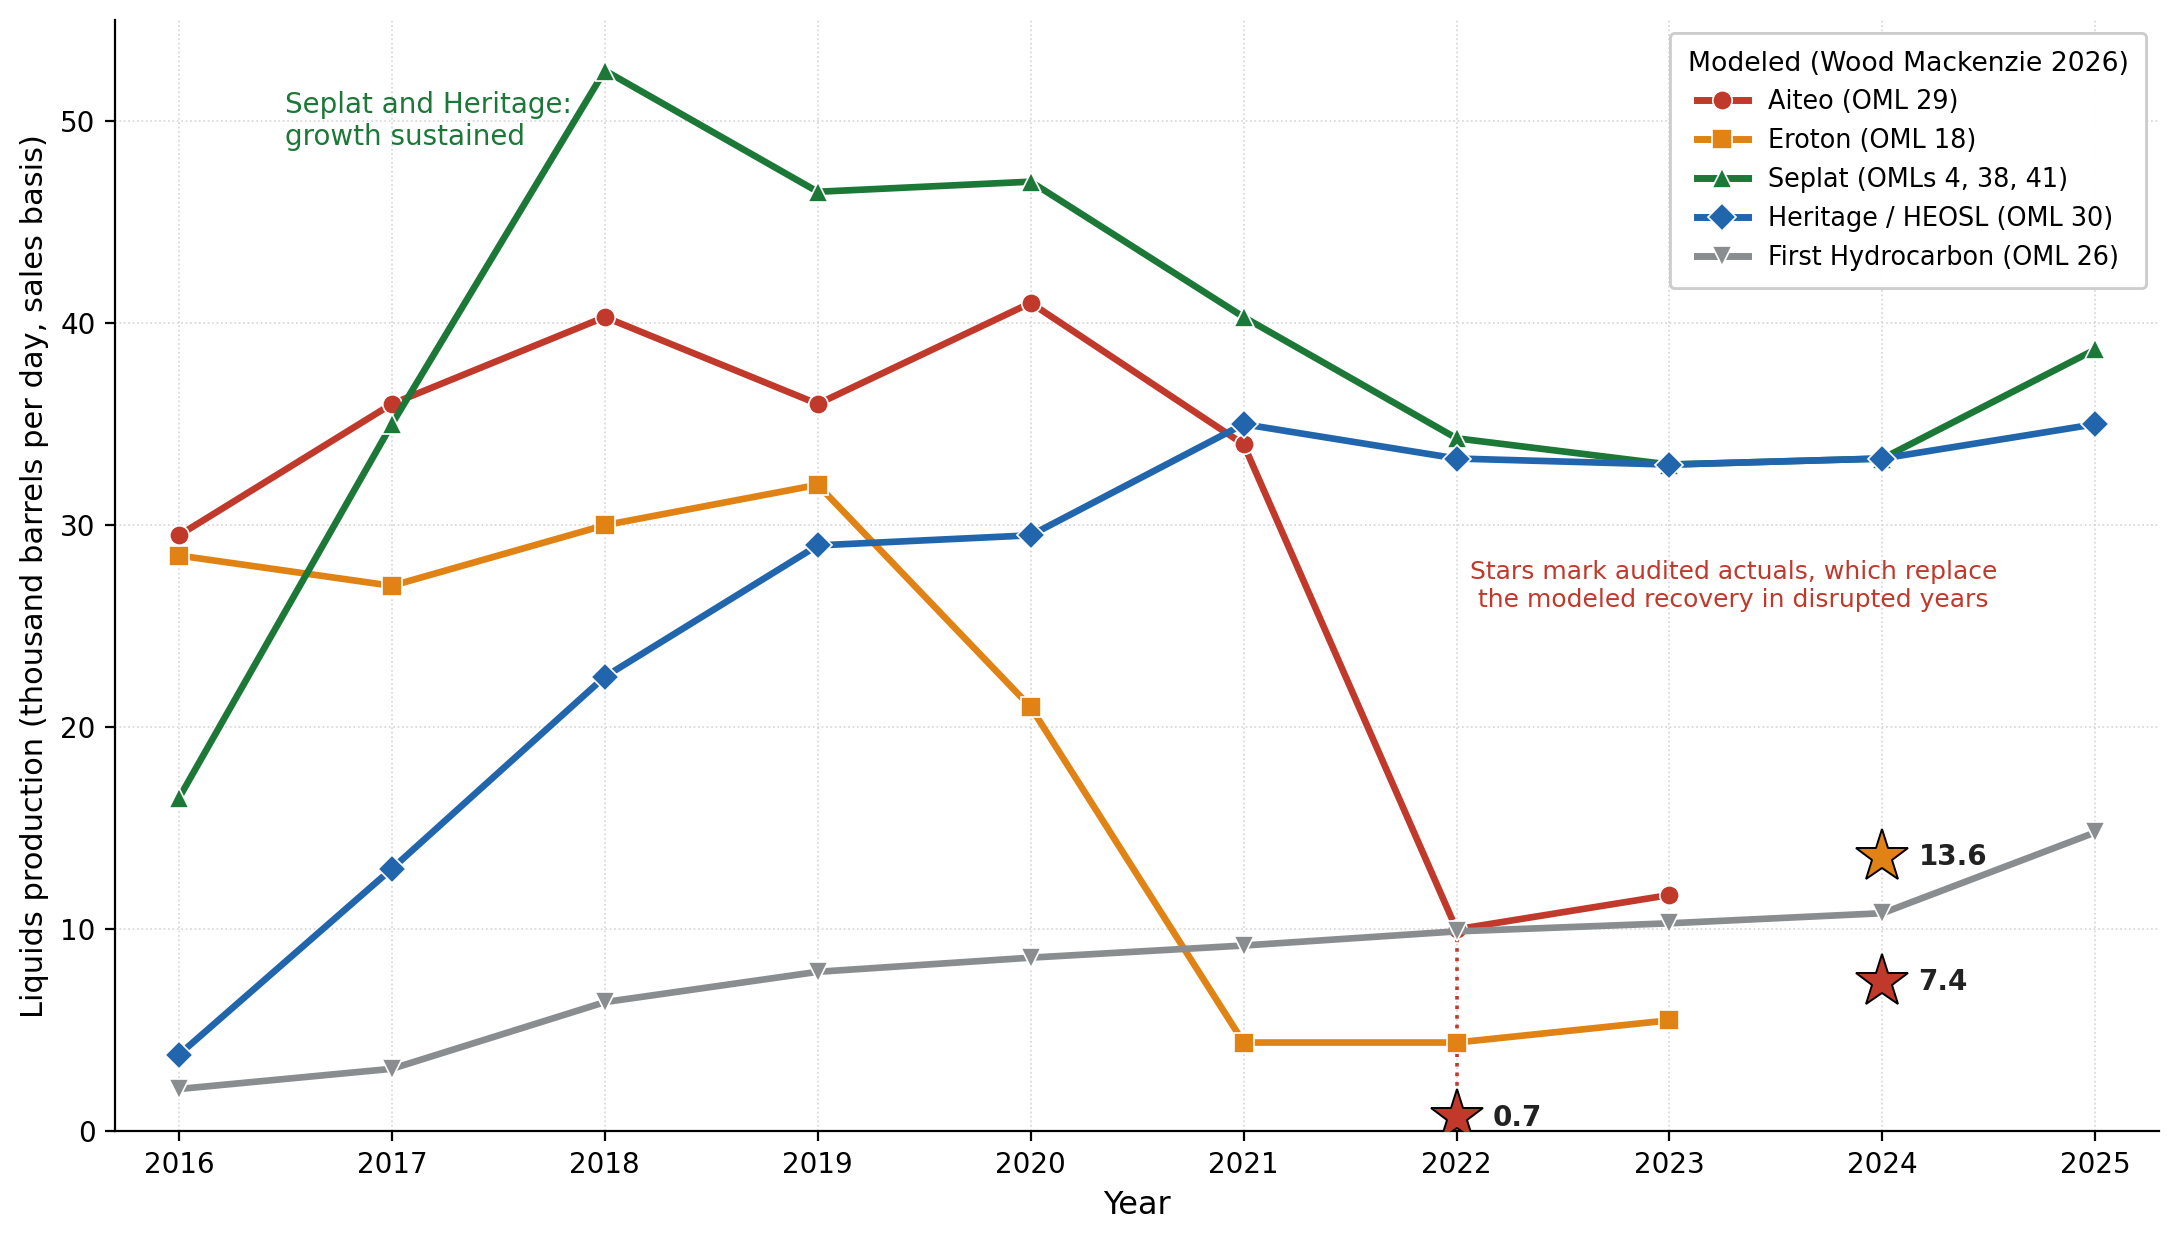
\includegraphics[width=\textwidth,height=0.45\textheight,keepaspectratio]{Figure_4_1_production_trajectories.png}
\caption[Post-divestment production trajectories of the formal case...]{Post-divestment production trajectories of the formal case OMLs. Lines show Wood Mackenzie (2026) modeled field liquids by license, on a sales basis after estimated theft; the Aiteo and Eroton lines stop at 2023, before a later modeled recovery the audited record does not support. Stars mark the audited or regulatory figures that govern in the disrupted years and fall well below the modeled lines. Where the two measurement bases diverge, the audited record governs. NPDC, the marginal cohort, and the design contrasts are omitted for want of a comparable license-level series.}
\end{figure}

\hypertarget{the-critical-experiment-aiteo-on-oml-29}{%
\section{The Critical Experiment: Aiteo on OML
29}\label{the-critical-experiment-aiteo-on-oml-29}}

Aiteo is the case where the competing explanations generate the most
divergent predictions. It is the operator that funded production growth
and then failed in a crisis beyond its capacity to contain, on an asset
acquired six years before the Petroleum Industry Act. Four of the five
explanations are tested here through their divergent predictions about
whether and how those two outcomes can co-occur in the same operator;
fiscal regime effects are eliminated separately by timing (Section
4.3.2). The documentary record adjudicates several of these differences
and bounds the rest. The positive case for capability-related factors is
built first, from the shape of the failure, before each competing
explanation is tested against its own falsification conditions; the
consolidated verdict for the case comes last (Section 4.3.6).

\hypertarget{the-selective-failure-pattern}{%
\subsection{The Selective Failure
Pattern}\label{the-selective-failure-pattern}}

Capability-related factors predict a particular shape of failure: the
knowledge-intensive parts of the operation fail while the routine parts
succeed. Routine production can often be sustained through established
procedures, contractor support, maintenance spending, and documented
operating knowledge, so an operator that inherited assets without the
embedded tacit knowledge to run them could still sustain output. The
same operator would falter when an event demanded the tacit judgment and
practiced routines that crisis response and well control require.
Aiteo's record is consistent with that shape.

On the routine side, production grew. The Wood Mackenzie modeled series
shows output on OML 29 rising over the post-acquisition years, from
about 30,000 barrels per day in 2016 to a peak near 41,000 in 2020.
Audited metered production reached 38,200 in 2021, the year before the
blowout (Wood Mackenzie, 2026; NEITI, 2021). Aiteo's announcement of a
90,000 barrel-per-day peak in March 2017 is a reported corporate figure
that sits well above the audited volumes. Part of the divergence between
reported peaks and audited volumes on the Bonny system reflects wellhead
potential measured before the pipeline-loss allocation that separates
gross from delivered crude. The gap here also exceeds what that
mechanism alone explains, and the argument holds without the figure. In
the crisis-response domain, the operation failed conspicuously. In
November 2021 the Santa Barbara Well 1 blew out and flowed uncontrolled
into the surrounding creeks until it was secured on December 8, roughly
33 days later. The joint investigation conducted by NOSDRA, the NUPRC,
the Bayelsa State Ministry of Environment, community representatives,
and well-control consultants attributed the blowout to third-party
interference. The affected community and the Bayelsa State Government
insisted that the cause was equipment failure (NOSDRA Joint
Investigation Visit, 2021; NOSDRA and NUPRC via Vanguard, 2021). The
cause is therefore contested, and the capability finding holds
independently of it. What the record establishes is a containment
failure. Aiteo assembled its well-control response after the fact,
engaging external specialists only once the blowout had occurred,
including Halliburton's Boots and Coots working with a local resource.
NOSDRA separately engaged Kenyon International for spill response, and
the well was secured only after about a month (Upstream Online, 2021;
Vanguard, 2021). The director-general of NOSDRA attributed the prolonged
failure to a capacity deficit, observing that operators forced to import
foreign well-control expertise lose critical time. He contrasted it with
the embedded arrangements an international operator carried, noting that
Shell had contained the 2011 Bonga spill quickly through a standing
worldwide spill-response subscription (NOSDRA via BusinessDay, 2021).
The investigation left the quantity spilled unsettled; independent
estimates put it near 200,000 barrels across some 41 communities, and
Aiteo disputed higher figures (NOSDRA Joint Investigation Visit, 2021;
SweetcrudeReports, 2021).

The well was a latent exposure well before it failed. Santa Barbara Well
1 had been non-producing since the 2015 acquisition; both Shell and
Aiteo left it undecommissioned, and it lay isolated, unplugged and
unmonitored, with further spills recorded in the area in 2018 and 2019.
Whether the blowout was triggered by tampering, as the official
investigation found, or by equipment failure, as the community alleged,
an idle well left in that state for six years was a standing hazard that
a fully resourced operator would have retired or kept under watch. The
capability reading turns on the containment failure that followed,
leaving the trigger aside.

Two inferences follow, and they rest on different evidence. First, the
funded production growth weakens capital constraints as the binding
explanation, in the sense of a single factor that alone accounts for the
outcome. The operator paid about \$2.562 billion for the 45 percent
interest in OML 29 and the Nembe Creek Trunk Line (HOMEF, 2021;
Nairametrics, 2015), and then funded sustained production growth
demonstrably had capital available for production-directed major
operational spending. That alone leaves open how Aiteo allocated funds
internally, so the failure turns on whether crisis readiness was
unavailable through financial scarcity or absent because the
organization had yet to put it in place. Second, and separately, the
failure points toward capability-related factors. That reading rests on
the operational evidence concentrated in the crisis-response domain,
with the funded growth bearing only on capital. That evidence is the
absence of a contingency plan, the absence of a standing well-control
contract, the dependence on contractors engaged after the fact, and the
well left undecommissioned and unmonitored. The reviewed record for the
OML 29 transaction shows no structured provision for retaining Shell
operating staff, well-control routines, or crisis-response systems.

The competing reading treats that operational evidence as a budgeting
choice: an operator with capital for production growth might simply have
declined to fund crisis readiness. The distinction matters, because a
choice to leave a known requirement unfunded is a management decision
while the absence of the readiness system altogether is a capability
gap, and both stand apart from capital constraints. The observable
evidence favors the capability reading over a pure financial-scarcity
reading. A standing well-control arrangement is a small commitment
relative to the cost of an uncontrolled blowout response, so a funds
shortage accounts poorly for its absence. The three weeks of improvised
response, in place of an executed plan, point the same way: to an
organization that had yet to institutionalize crisis readiness before
the event. Capital constraints are rejected as sufficient regardless of
which reading holds, because the funds for production growth
demonstrably existed.

The leadership's background helps make the capability reading plausible,
though on its own it leaves unproven that the gap caused the failure.
Aiteo's founder and chief executive, Benedict Peters, holds a degree in
geography and regional planning and built his career in downstream
petroleum, in trading, storage, and fuel distribution, his upstream
exploration and production experience beginning only with the
acquisition of OML 29. The downstream-only background carries less than
proof on its own; it is a mechanism-consistency indicator, since the
failure fell in the upstream well-control domain that lay outside that
experience. The operational record is the evidence that the gap operated
in practice.

\hypertarget{fiscal-regime-effects}{%
\subsection{Fiscal Regime Effects}\label{fiscal-regime-effects}}

Fiscal regime effects fail on timing. Aiteo acquired OML 29 in 2015, and
the Petroleum Industry Act was enacted on August 16, 2021, six years
later. The conditions that produced the failure were in place well
before that date: the suspended well had been left undecommissioned
since 2015, and the unremediated spills date from 2018 and 2019. A cause
must precede its effect. The blowout itself came in November 2021, three
months after the Act, but the conditions it exposed, the absent
well-control capability, the missing contingency plan, and the prior
unmanaged incidents, all predated the Act. Fiscal regime effects are
therefore rejected for this case as the primary explanation for the
observed failure.

\hypertarget{regulatory-inadequacy}{%
\subsection{Regulatory Inadequacy}\label{regulatory-inadequacy}}

The regulatory framework in force at the time of the Aiteo transaction
left operational capability outside its screen. Section 29 of the
Petroleum Act required ministerial consent to assign an Oil Mining Lease
but stopped there, leaving the buyer's ability to run the asset
untested. On the necessary-condition test, the framework indeed omitted
a capability requirement.

What the regulator did next points to a gap in the framework's content.
The rules were applied as written; what they required was too little. In
2024 the NUPRC introduced a seven-pillar divestment framework that it
described as the first of its kind in the sixty-eight-year history of
Nigerian exploration and production. Its first pillar, technical
capacity, appeared for the first time, with the Petroleum Act, internal
guidelines, and practice all silent on it before. That the NUPRC created
a capability criterion is strong evidence that the criterion was new,
and the new framework produced operational consequences beyond a
statement of intent. A divestment was initially withheld pending
assessment, and decommissioning escrow exceeding \$400 million was
secured across the 2024 transactions. Post-divestment failures
contributed to the timing of the reform, but the content of the reform,
a specific technical-capacity test new to the framework, is the mark of
a recognized design failure.

The gap's existence, on its own, sits below proof that it caused the
Aiteo failure. Causation would require that a capability gap was
identifiable at the point of transfer and non-compensable through the
market afterward. The first, identifiability at the point of transfer,
is directly supported. NOSDRA's account that containing the blowout
exceeded the operator's available capacity, the after-the-fact
engagement of external specialists, and the absent contingency plan all
concern well-control capability, which is assessable before a transfer.
An audit at the point of transaction could have tested for well-control
protocols, crisis-response arrangements, and blowout contingency
planning. The second, non-compensability through the market afterward,
is suggested by the persistence of the gap across six years of operation
and is tested across the cases that follow (Sections 4.4 and 4.7). And
the same pre-2024 regulatory framework, the Petroleum Act and DPR
oversight, governed Seplat, HEOSL, Aiteo, and NPDC; as the cases that
follow show, their outcomes diverged, so the framework permitted the
failure while leaving open which operators would fail. For the single
case, then, regulatory inadequacy is consistent with the design-gap
interpretation: an enabling condition that permitted the failure while
leaving unexplained, on its own, why Aiteo failed where others held.
Whether the absence of capability screening is necessary across the
population is a question the cross-case synthesis takes up (Section
4.7).

\hypertarget{political-economy-at-the-case-level}{%
\subsection{Political Economy at the Case
Level}\label{political-economy-at-the-case-level}}

The political-economy explanation is tested here for Aiteo specifically,
through observable case-level indicators. The population-level
association reported by Rexer (2025) supplies context, and the test here
draws on the case record. The relevant indicators are board composition,
shareholding, and any change in the theft rate on OML 29 around the
transfer. For Aiteo, the available record supports only a weak test of
those indicators: corporate registry detail on board composition and
shareholding is incomplete, and the search recovered no
operator-specific theft-rate series around the transfer. The test here
is therefore narrower, whether political access, even if present, could
explain the non-substitutable well-control failure.

The decisive consideration is where political access substitutes for
capability and where it reaches its limit. Connections can plausibly
reduce certain exposures, oil theft, or community friction managed
through elite-mediated access, the substitutable dimensions. Well
control and blowout contingency rest on experiential knowledge, and on
this non-substitutable dimension the outcome turns on what an operator
actually holds. The Aiteo record splits along exactly that line.
Whatever connections may have done for theft or community access on OML
29, preventing or containing the Santa Barbara blowout turned on
well-control capability, which only operating experience supplies.
Political economy is therefore rejected as sufficient for operational
quality on the non-substitutable dimension. It may help account for
commercial survival, since Aiteo continued operating after the blowout,
while the onset of the blowout and the operator's inability to contain
it lie outside its reach. The positive form of the test, whether
connections sustain commercial viability while operational quality stays
poor, is developed on NPDC (Section 4.5.3).

\hypertarget{coordination-failure}{%
\subsection{Coordination Failure}\label{coordination-failure}}

Coordination failure, treated throughout as an observable feature of
unsuccessful cases and a symptom of deeper causes, is tested here
against persistence and failure type. The blowout occurred in November
2021, six years after the 2015 acquisition, well beyond a short
transition period. If coordination failure were merely a transition
problem, it should appear early and ease as the operator stabilizes.
Aiteo's pattern points the other way: specific knowledge-intensive
functions failed while routine production grew, and the failure
persisted for six years. The unresolved spills of 2018 and 2019 show the
exposure persisting years before the blowout, present at year three and
still unaddressed at year six.

A failure of this duration and this shape runs counter to a coordination
problem that self-corrects through operational learning, so coordination
failure is rejected as an independent cause for this case. Its
persistence and domain-specificity are consistent instead with a
structural absence of knowledge.

\hypertarget{the-aiteo-verdict}{%
\subsection{The Aiteo Verdict}\label{the-aiteo-verdict}}

The five explanations, and the coordination feature that accompanies
them, resolve as follows for the Aiteo case. The verdicts use the
categories specified in Chapter 2 (Section 2.6), and each rests on the
explanation's own evidence, with the elimination of rivals set aside.

\begin{longtable}[]{@{}
  >{\RaggedRight\arraybackslash}p{(\columnwidth - 6\tabcolsep) * \real{0.2500}}
  >{\RaggedRight\arraybackslash}p{(\columnwidth - 6\tabcolsep) * \real{0.2500}}
  >{\RaggedRight\arraybackslash}p{(\columnwidth - 6\tabcolsep) * \real{0.2500}}
  >{\RaggedRight\arraybackslash}p{(\columnwidth - 6\tabcolsep) * \real{0.2500}}@{}}
\caption[Verdicts for the Aiteo critical experiment on OML 29]{Verdicts for the Aiteo case on OML 29, the critical experiment, where funded production growth alongside an uncontained blowout rejects the capital, fiscal, and political-economy explanations as sufficient for the integrity failure and leaves capability-related factors most consistent with the evidence.}\\
\toprule\noalign{}
\begin{minipage}[b]{\linewidth}\RaggedRight
Explanation
\end{minipage} & \begin{minipage}[b]{\linewidth}\RaggedRight
Verdict
\end{minipage} & \begin{minipage}[b]{\linewidth}\RaggedRight
Evidence anchor
\end{minipage} & \begin{minipage}[b]{\linewidth}\RaggedRight
What would change this verdict
\end{minipage} \\
\midrule\noalign{}
\endfirsthead
\toprule\noalign{}
\begin{minipage}[b]{\linewidth}\RaggedRight
Explanation
\end{minipage} & \begin{minipage}[b]{\linewidth}\RaggedRight
Verdict
\end{minipage} & \begin{minipage}[b]{\linewidth}\RaggedRight
Evidence anchor
\end{minipage} & \begin{minipage}[b]{\linewidth}\RaggedRight
What would change this verdict
\end{minipage} \\
\midrule\noalign{}
\endhead
\bottomrule\noalign{}
\endlastfoot
Capital constraints & Rejected as sufficient & \textasciitilde\$2.562B
acquisition, 45\% interest plus the Nembe Creek Trunk Line (HOMEF, 2021;
Nairametrics, 2015); audited metered growth to 38.2 kb/d (2021)
alongside the crisis failure, modeled peak near 41 kb/d; capital
demonstrably available for production-directed major operational
spending & Evidence that crisis-readiness funding was cut for financial
reasons \\
Fiscal regime effects & Rejected for this case & Transaction closed
2015; PIA enacted August 2021; the capability gap predates the Act &
None; the timing is arithmetic \\
Regulatory inadequacy & An enabling condition insufficient on its own;
system-level role tested in the cross-case synthesis (4.7) & Section 29
lacked capability criteria; the NUPRC created them in 2024; the same
pre-2024 framework produced different outcomes across operators,
developed in the cases that follow & Evidence that the framework
screened for capability and that Aiteo passed \\
Political economy & Rejected as sufficient for operational quality
(non-substitutable dimension) & Preventing or containing the blowout
required well-control capability beyond the reach of connections &
Evidence that political interference directly caused the operational
failure, beyond enabling commercial survival \\
Coordination failure & Rejected as independently caused; an observable
feature of the unsuccessful cases & Persistence at six years;
domain-specific failure; unremediated prior incidents & Evidence of a
specific coordination breakdown independent of knowledge absence \\
Capability-related factors & Most consistent with the evidence for this
case & Selective failure signature; containment failure lasting about a
month, which NOSDRA attributed to a capacity deficit; after-the-fact
reliance on external well-control specialists against absent embedded
crisis-response arrangements; six-year persistence; the documents
reviewed silent on any structured knowledge-transfer provision in the
transaction & An operator without inherited upstream knowledge handling
a comparable crisis successfully \\
\end{longtable}

Across the two outcome dimensions, the diagnostic split is clean for the
period the critical experiment turns on. In the years before the
blowout, commercial production grew while crisis-readiness stayed
absent, and the explanation most consistent with that split is one that
bears on integrity, with funding set aside, since binding capital
constraints would have suppressed production too. Output then fell
sharply after the blowout, to about 4,900 barrels per day metered in
2022, 700 fiscalized (NEITI, 2022), so the capability failure spread to
both dimensions; that loss came after the blowout, so the
capital-constraints explanation stays closed. In the terms of Chapter 2
(Section 2.2), this is a failure of the asset as a sociotechnical
system. The transaction moved the wells but not the operating
organization that had run them, and when the well reached a crisis the
well-control capability, the standing contracts, and the practiced
crisis response that the operating organization carried were not present
to contain it. This verdict reflects pattern consistency for a single
case.

Appendix E reproduces this verdict matrix for every case, recording the
evidence, confidence level, and falsification condition behind each
verdict; the analyses that follow state their verdicts in prose and
refer to that appendix for the full matrices.

\hypertarget{cross-case-validation-failure-replication-and-regulatory-screening}{%
\section{Cross-Case Validation: Failure Replication and Regulatory
Screening}\label{cross-case-validation-failure-replication-and-regulatory-screening}}

The Aiteo verdict rests on a single case. Two further operators test
whether it holds. Eroton acquired OML 18 from the same seller in the
same divestment round and, like Aiteo, grew production before losing it,
which makes it a replication candidate. Its collapse, however, ran
partly through a shared export line whose chronic, theft-driven downtime
lay largely outside Eroton's control, so the case is a partial
replication, complicated by the shared line (Section 4.4.1). First
Hydrocarbon acquired OML 26 through a buyer whose executives were later
convicted of fraud, which interrupts any reading of its operational
capability but bears directly on whether the approval process screened
buyers at all (Section 4.4.2).

\hypertarget{eroton-on-oml-18-a-partial-replication-complicated-by-a-shared-trunk-line}{%
\subsection{Eroton on OML 18: A Partial Replication Complicated by a
Shared Trunk
Line}\label{eroton-on-oml-18-a-partial-replication-complicated-by-a-shared-trunk-line}}

Eroton's early trajectory mirrored Aiteo's: acquisition from the same
2015 Shell divestment, rapid production growth, and a later collapse. A
consortium led by Midwestern Oil and Gas, with the Canadian-listed Mart
Resources and Suntrust Oil and Gas, acquired a 45 percent interest in
OML 18 from Shell, Total, and Eni in March 2015 for about \$1.2 billion.
NNPC held the remaining 55 percent, and Eroton was the designated
operator (Mart Resources, 2015; Templars, 2015). Production then grew
from a low base, and two independent sources agree on its scale and
trajectory once measurement basis is held constant. Wood Mackenzie's
modeled series puts the field near 32,000 barrels per day at its 2019
peak. The operator's own disclosures, released through its listed
financier San Leon, report full-field gross output before pipeline
losses of roughly 39,000 to 45,000 barrels per day across 2017 to 2019,
about 50,000 on a producing-day basis. Delivered sales after downtime
and allocated losses came to roughly 26,000 to 31,000 (Wood Mackenzie,
2026; San Leon Energy, 2017; 2019; 2020). The spread between these
figures follows from the measurement bases: the difference between
wellhead potential, annual gross, and the volume that survived a
pipeline-loss wedge running between 26 and 35 percent in these years.
The crude-reconciliation mechanism Wood Mackenzie documents for the
entire Bonny system and that Eroton addressed by installing
custody-transfer metering in 2018 (San Leon Energy, 2019; Wood
Mackenzie, 2026). On production and technical cost, Eroton looked
competent for several years, and NNPC recognized it as one of two
operators with the lowest technical cost per barrel (Wood Mackenzie,
2026). That initial competence separates Eroton from Aiteo, where the
well-integrity exposure later implicated in the blowout existed from
acquisition, and it is the first reason to treat Eroton as a partial
replication, short of a literal one.

The composition of the acquiring consortium is a secondary,
mechanism-consistency indicator, set out here because the verdict that
follows relies on it. Financial and business-development principals
assembled Eroton, in place of former international-oil-company
operators. Its lead figure, Onajite Okoloko of Midwestern Oil and Gas,
holds a degree in economics and a Harvard management qualification and
built his career in corporate finance and oilfield services. He was
managing director of Oando Energy Services, then in a marginal field
through Midwestern and in fertilizers through Notore, his career falling
outside well engineering and reservoir management (Africa Oil \& Gas
Report, 2013; 2015). The contrast with Seplat guards against an easy
objection. Okoloko had operated a marginal field, Midwestern's Umusadege
at about 13,000 barrels per day, just as Seplat's Austin Avuru had run
Platform Petroleum, so marginal-field experience was common to both.
What differed was that Avuru carried three decades of hands-on petroleum
engineering and reservoir management that scale to a complex asset,
where a business-development background scales less readily.
Marginal-field success was a necessary condition for a major lease, one
step on a longer path. The consortium that took OML 18 held the
financial and commercial capability to fund and acquire the asset, while
the inherited upstream operating depth to improvise under stress lay
beyond it. The background falls below proof that this gap caused the
failure; the internal record does that work.

Then delivered output fell to almost nothing. Export volumes collapsed
through 2020 and 2021, and by the time NNPC removed Eroton as operator
in March 2023 the asset had delivered near-zero export volumes for
roughly two years (NNPC via BusinessDay, 2023). The NEITI-audited figure
for 2021 had already fallen to about 19,300 barrels per day. Wood
Mackenzie's throughput record for the Bonny system shows the OML 18
evacuation fields, Cawthorne Channel and the OML 18 portion of Awoba
among them, dropping to zero from 2021, which corroborates the delivery
collapse from a source independent of the operator (NEITI, 2021; Wood
Mackenzie, 2026). The 2022 audit makes the split explicit: OML 18
metered about 9,000 barrels per day at the flow station but fiscalized
only 600 after a terminal adjustment of 1.6 million barrels, the
wellhead-to-delivered gap that defines evacuation stranding (NEITI,
2022). The collapse ran through two distinct pathways, and separating
them is the work of this case.

The first pathway is external, and it lay largely outside Eroton's
control. The Nembe Creek Trunk Line, the export route for OML 18 crude,
went into force majeure from the fourth quarter of 2021, and every
operator that depended on it went without deliveries (San Leon Energy,
2022; 2023). The line's unavailability extended well beyond that
quarter. Wood Mackenzie records the Nembe Creek Trunk Line as frequently
targeted by vandals and militant groups, with downtime that can reach 60
percent, and notes that the \$1.1 billion line Shell rebuilt in 2010
specifically to deter theft proved similarly ineffective against it.
Terminal force majeure on the Bonny system, the same source observes,
follows generically from vandalism or sabotage against the trunk
pipelines, a system-wide hazard that falls on every operator on the line
alike (Wood Mackenzie, 2026). The vulnerability was therefore structural
to the asset and the region, it predated Eroton and Aiteo alike, and it
transferred with the hardware from Shell, which had itself repeatedly
shut the line to remove theft points. Eroton kept producing at the
wellhead through the force majeure, reporting on its own account about
500,000 barrels in November 2021, an interested-source figure of roughly
16,700 barrels per day for the month. The crude meanwhile stayed short
of the Bonny terminal (San Leon Energy, 2023). The gap between metered
wellhead volume and delivered volume is the signature of evacuation
stranding: the crude is produced and metered, then held before it can be
delivered.

The line that stranded Eroton's crude was operated by Aiteo on OML 29, a
link of shared exposure to the same line. The official joint
investigation into the contemporaneous Santa Barbara incident attributed
it to third-party interference (Section 4.3), and the trunk-line force
majeures recur on the same third-party-sabotage pattern across operators
and across the periods before and after Aiteo took the line. The
available record leaves any Aiteo maintenance or surveillance failure on
the line inseparable from the regional theft and sabotage that afflict
it. The evacuation shock therefore reads best as the common environment
that every Bonny-system operator faced, a feature of the asset more than
of either operator's capability. A community suit now before the Federal
High Court alleges that Aiteo's trunk-line spills reflected operational
negligence and a failure to replace corroded pipelines, which, if
established, would reopen that reading. As of this writing the suit is
pending, with a finding yet to be made (Opu Nembe Kingdom v Aiteo,
FHC/YN/CS/284/2024).

The second pathway is internal and concerns whether Eroton could mount
an organizational response to that shock. The Federal Inland Revenue
Service sealed the company's head office for more than twelve months
over unpaid taxes; the EFCC and NUPRC opened investigations; and an NNPC
forensic audit identified governance failures (NNPC via BusinessDay,
2023; NNPC via Leadership, 2023). Most directly, an alternative barge
evacuation route won approval, and Eroton left it unexecuted, so the
crude beyond the trunk line's reach stayed stranded under the sanctioned
workaround as well (San Leon via Energy Voice, 2019, 2022a, 2022b).
These are organizational-performance failures, and they fall in the part
of the operation that Chapter 2 treats as organizational capability:
managing a regulator, sustaining joint-venture governance, and executing
a complex logistics alternative under stress are capability tasks, the
organizational work that sits above the wellhead. They are consistent
with an organizational-capability gap. The documentary record alone,
however, leaves that reading entangled with governance, liquidity, or
political dynamics, and participant testimony is the evidence that would
distinguish them.

The two pathways resist clean separation, and the case is weaker for it.
The external shock alone could have stranded a capable operator; the
internal failures alone could have sunk production even with the trunk
line intact. In the event both occurred together, and the documentary
record can only partly apportion how much of the two-year collapse each
contributed. That is the honest limit of the case, and it is why Eroton
corroborates the Aiteo pattern while leaving it unconfirmed.

Within that limit, the explanation tests run as follows. Capital
constraints are rejected as sufficient. The growth to a modeled 32,000
barrels per day, corroborated by the operator's reported gross output,
demonstrates that capital was available for production-directed major
operational spending. An operator that funded that growth held the funds
to run the asset (Wood Mackenzie, 2026; San Leon Energy, 2019). NNPC
separately stated that the joint-venture partners met their funding
obligations through the decline. That statement carries a caveat,
because NNPC made it while removing Eroton as operator, a context in
which it had an interest in placing the failure on the operator over
joint-venture underfunding. The inference against capital constraints
therefore rests more securely on the documented production growth than
on the statement. The unpaid-tax evidence may indicate liquidity stress
or governance failure, though on its own it leaves open whether the
joint venture held the capital to sustain production or to execute the
evacuation alternatives, so the verdict stands. Eroton's own rebuttal
accepted that funding was maintained; it attributed the collapse to the
trunk-line force majeure (Eroton via Petroleum Africa, 2023). Fiscal
regime effects are rejected for this case. The production deterioration
began before the Petroleum Industry Act, and the acquisition,
capability, and evacuation-dependence conditions that produced it were
all established under the pre-Act regime. The Act, enacted in August
2021, postdates the conditions that produced the collapse and stays
outside the primary explanation, even though the removal of the operator
ran into 2023. The regulatory framework in force at the 2015 acquisition
left operational and organizational capability outside its screen, the
same design gap documented for Aiteo. It permitted Eroton's acquisition
while, applying alike to every operator, leaving unexplained why Eroton
specifically collapsed, and it functions here as an enabling condition
shared across operators, short of a differentiating cause. Coordination
failure is rejected as independently caused: the collapse came six to
eight years after acquisition, well beyond a short transition period,
and a transition problem should appear early and ease as the operator
settles. Here, by contrast, the operator demonstrated routine
operational competence for several years before the collapse.

The political-economy and capability readings are harder to separate
here than at Aiteo, and the evidence is thinner. Corporate registry
detail on Eroton's board composition and shareholding is incomplete, so
the question is carried by the non-substitutability logic, the registry
record being too incomplete for a direct case-level test. Political
economy remains live for the case as a whole; it could plausibly bear on
the unpaid taxes, the regulatory treatment, or access to approvals. It
is rejected only as a sufficient explanation for the
operational-capability tasks at issue, in particular executing the
approved barge alternative, which lay beyond political access. The
capability reading is consistent with the internal pathway but not
decisive for the case, because the external trunk-line shock confounds
the attribution. The consortium's business-development composition,
established above, supports the reading only as a secondary indicator:
it is consistent with an organization that ran routine production well
while struggling to improvise an operational response under stress. The
background indicates the gap without establishing it as the cause; the
operational record in each case establishes the link.

Eroton therefore replicates the Aiteo pattern in part. An operator
without inherited upstream technical depth grew routine production and
then faltered when conditions deteriorated, which matches the Aiteo
trajectory. The collapse, however, mixed an external evacuation shock
with internal governance failure, and the evidence attributes it to
capability with less confidence than the Aiteo case permits. The verdict
reflects that ambiguity.

Appendix E records the full verdict matrix for the case, with the
evidence and the falsification condition behind each verdict.

The case adds two findings without amounting to a second proof. It
rejects capital constraints and fiscal timing on the same logic as
Aiteo, and it shows the funded-growth-then-failure pattern recurring in
a second operator assembled without inherited upstream depth. The
evacuation shock that might have supplied a second, independent line of
evidence instead confounds the capability attribution: it ran through
the trunk line as the common environment every Bonny-system operator
faced, structurally theft-driven and inherited from the seller. Whether
the pattern holds where the conditions differ on knowledge inheritance
is what the theoretical replications test, against operators facing the
same evacuation environment (Section 4.5).

\hypertarget{first-hydrocarbon-on-oml-26-a-test-of-regulatory-screening}{%
\subsection{First Hydrocarbon on OML 26: A Test of Regulatory
Screening}\label{first-hydrocarbon-on-oml-26-a-test-of-regulatory-screening}}

First Hydrocarbon Nigeria acquired a 45 percent interest in OML 26, in
the western Niger Delta, from the Shell joint venture in 2011,
completing an agreement struck in October 2010. The interest combined
the holdings of Shell at 30 percent, Total at 10 percent, and Eni at 5
percent, with the state company NPDC holding the remaining 55 percent
(First Hydrocarbon Nigeria, 2011; Wood Mackenzie, 2026). Two features
set the case apart from Aiteo and Eroton. First Hydrocarbon Nigeria was
a special-purpose vehicle created by the London-listed Afren plc to hold
Nigerian upstream assets, and Afren held 45 percent of it at completion,
rising to 70 percent by the time the company failed (Upstream Nigeria,
2018). And First Hydrocarbon Nigeria never operated OML 26: NPDC
asserted operatorship under a first-refusal clause in the joint
operating agreement and ran the asset throughout, with a joint
asset-management team formed only in 2016 (Africa Oil and Gas Report,
2012; Acha et al., 2019). The buyer was a non-operating financial
partner whose sponsor collapsed through fraud, a corporate failure that
played out entirely away from the asset's operations. For both reasons
the case lies outside a test of the buyer's operational capability, and
it enters here as a screening case. What it tests is whether the
approval framework assessed buyer fitness, and it provides the cleanest
rejection of capital constraints in the case set.

The screening question turns on the statute, and the statute is
explicit. Section 29 of the Petroleum Act required ministerial consent
to assign the lease while leaving the acquirer's fitness, capability,
and governance untested, the same statutory void documented for the
Aiteo transfer (Section 4.3.3). The buyer commanded ample capital and
corporate standing: Afren was a FTSE 250 company that peaked near \$2.6
billion in market value. First Hydrocarbon Nigeria funded the
acquisition and its initial development share through \$280 million of
facilities (First Hydrocarbon Nigeria, 2011; UK Serious Fraud Office,
2018). The acquiring entity's gap lay in corporate governance integrity,
a dimension that the approval framework reviewed here left outside any
party's remit, at approval and through any ongoing post-transfer fitness
test. Within four years of completion, Afren had collapsed into
administration, in July 2015. Its two most senior executives, the chief
executive Osman Shahenshah and the chief operating officer Shahid Ullah,
were convicted in 2018 of fraud and money laundering for a scheme they
ran while leading the company. They diverted roughly \$45 million from a
\$300 million transaction with another Nigerian partner into a Caribbean
or Bermudan shell company they controlled (UK Serious Fraud Office,
2018). The convictions stood when the Court of Appeal refused permission
to appeal in 2019, and a confiscation order of £5.45 million followed in
2020 (Court of Appeal, 2019; Energy Voice, 2020). The case leaves open
whether a Nigerian regulator would necessarily have discovered the fraud
in 2010 or 2011; it shows that the approval framework lacked any
explicit buyer-fitness or governance-integrity screen capable of making
that question part of the approval decision. The cost of the collapse
reached beyond Afren's shareholders: Nigerian banks that had lent into
the structure lost an estimated \$185 million when the company failed
(Vanguard, 2015).

Capital constraints are rejected as sufficient. The binding-constraint
version of the capital explanation requires that a shortage of funds
prevented the acquirer or the venture from running or developing the
asset. Here the acquirer commanded the resources of a
multi-billion-dollar listed company and dedicated financing facilities,
and the venture failed regardless, through a governance fraud that stood
apart from funding scarcity. Capital abundance left both the failure and
the asset's performance untouched.

Appendix E records the case's verdicts, including the dimensions it
leaves not tested, with the evidence and the falsification condition for
each.

Because NPDC operated OML 26, the asset's production reflects the state
operator's performance, the buyer's role aside. The modeled and audited
records agree that OML 26 produced only two to three thousand barrels
per day through the mid-2010s and reached roughly eight to ten thousand
around 2020 to 2021. The audited record then shows output slipping back,
well below the asset's developed capacity throughout (Wood Mackenzie,
2026; NEITI, 2020, 2022). That trajectory bears on NPDC's operatorship,
taken up in Section 4.5.3, with the buyer's inherited capability set
aside.

The case adds a dimension that neither Aiteo nor Eroton supplies. At
Aiteo the screening gap permitted an operator that proved unable to
contain a crisis. Here the same statutory gap permitted an acquirer
whose leadership was later convicted of serious fraud committed while
running the company, on an asset where the buyer never took operational
control. The two cases together show that the pre-2024 framework left
acquirers unscreened for both operational capability and governance
integrity, the void the NUPRC moved to close in 2024 (Section 4.3.3).
And the case rejects capital constraints in their starkest form, since
here the buyer held every financial advantage and failed anyway. Whether
the capability pattern that the critical experiment identified holds
where a capable operator inherits and runs the asset is the question the
theoretical replications take up next (Section 4.5).

\hypertarget{theoretical-replication-operators-that-differed-on-capability}{%
\section{Theoretical Replication: Operators That Differed on
Capability}\label{theoretical-replication-operators-that-differed-on-capability}}

The critical experiment identified a capability-related failure at
Aiteo, and the partial replication at Eroton showed a similar
funded-growth-then-collapse pattern, though there the attribution was
confounded by an external evacuation failure the documentary record
leaves entangled with internal governance (Section 4.4.1). Literal
replication predicts the same outcome where the same condition holds;
theoretical replication predicts a contrasting outcome where the
condition differs, and for a reason the theory names (Yin, 2009). The
three cases here differ from Aiteo and Eroton on capability. Seplat
acquired its leases with an experienced founding team and a technical
partner, and the capability account predicts sustained production and
integrity (Section 4.5.1). OML 30 supplies a within-asset comparison in
which the asset, owners, regulatory regime, and fiscal terms held
constant while operatorship passed from the state company to an
indigenous operator with technical capability, which isolates operator
capability more sharply than any cross-operator comparison can (Section
4.5.2). NPDC operated its acreage as a state company and underperformed
while surviving commercially, which tests political economy in the
positive form left open earlier (Section 4.5.3). All three operated
under the same pre-2024 regulatory regime as the failure cases, NPDC as
a state entity under, if anything, weaker external discipline, so the
contrast among them also tests whether regulatory inadequacy, common to
every operator, can account for outcomes that diverge.

\hypertarget{seplat-on-omls-4-38-and-41-a-founding-teams-technical-depth}{%
\subsection{Seplat on OMLs 4, 38, and 41: A Founding Team's Technical
Depth}\label{seplat-on-omls-4-38-and-41-a-founding-teams-technical-depth}}

Seplat entered upstream operations with the technical depth the failure
cases lacked, and it sustained both production and operational
integrity, the outcome the capability account predicts for a capable
operator. The case is the first theoretical replication.

Seplat Petroleum Development Company acquired a 45 percent interest in
OMLs 4, 38, and 41 from the Shell joint venture in 2010 for about \$340
million (Seplat, 2014). The depth originated with the buyer. The
reviewed record for the 2010 transaction shows no structured
capability-transfer provisions, and the knowledge that ran the assets
came from the founding team's own prior careers. Austin Avuru, the
founding chief executive, had spent more than three decades in Nigerian
petroleum engineering and reservoir management, beginning at NNPC as a
wellsite geologist and reservoir engineer and later running the
marginal-field operator Platform Petroleum. Basil Omiyi, who had led
Shell's Nigerian operations, joined the board after the founding
(Seplat, 2014). Where Eroton's principals brought a business-development
background, Seplat's brought operating depth, and the company paired it
with a technical partnership with Maurel et Prom, an established
international operator (Seplat, 2014). The founding team and the
partnership together gave Seplat the absorptive capacity to run the
assets, the buyer-side condition specified in Chapter 2; capability was
present at the buyer from the start, brought by the founding team
itself.

Production grew and held. The Wood Mackenzie modeled series puts the
three leases near a combined 53,000 barrels per day at their 2018 peak,
and the audited record shows metered production of 42,300 in 2021 and
43,100 in 2020. The modeled series holds the leases near 39,000 in 2025,
about 74 percent of peak and inside the sustained band (Wood Mackenzie,
2026; NEITI, 2020, 2021). Where Aiteo and Eroton fell to small fractions
of their post-acquisition peaks (Section 4.2), Seplat held above 70
percent of its own.

The available integrity indicators point in the same direction, though
they rest on different measurement bases. Seplat reported more than 11
million man-hours without a lost-time injury and was named AfriSAFE
Energy Company of the Year in 2024, and its joint-venture flaring ran
below the indigenous-operator figures in the 2021 audit (NEITI, 2021;
Seplat Energy, 2024). The flaring comparison is confounded by
gas-evacuation infrastructure and carries little decisive weight, and
the award is a form of recognition, carrying less evidentiary weight
than the audited regulatory data, so the indicators support the reading
jointly, as a set. Set against Aiteo's uncontrolled blowout and the
weaker integrity indicators in the failure cases, Seplat's safety record
points in the expected direction and is consistent with the capability
account.

A later seller-independence check points the same way and is developed
in the cross-case synthesis (Section 4.7). In 2024 Seplat acquired Mobil
Producing Nigeria Unlimited from ExxonMobil and integrated a producing
asset from a different seller (Seplat Energy, 2024, 2026). Because that
transaction is only months old, it stands outside the historical
evidence here; the absorptive-capacity reading rests on the fifteen-year
record of the 2010 leases, and the MPNU integration enters as a design
contrast, short of a second case.

The case establishes that a buyer with inherited technical depth, under
the same regulatory and fiscal regime as the failure cases, sustained
the outcomes that eluded the failure cases. The case leaves open which
capability element, the founding team or the Maurel et Prom partnership,
was decisive, since both were present throughout. The three leases also
differ in asset characteristics from OML 29, so the comparison is one of
operator type under common institutional conditions, a contrast short of
a matched-asset experiment.

The full verdicts for this case are in Appendix E. The question for the
alternatives is whether any of them accounts for why Seplat succeeded
where capability-poor operators failed.

Seplat's outcome matches the capability prediction. An operator that
brought the technical depth Aiteo and Eroton lacked produced the
sustained production and operational integrity that eluded them, under
the same regime that governed them all.

\hypertarget{oml-30-a-within-asset-operator-change}{%
\subsection{OML 30: A Within-Asset Operator
Change}\label{oml-30-a-within-asset-operator-change}}

OML 30 offers the strongest control available in this study. The asset,
its owners, the regulatory regime, and the fiscal terms all held
constant while operatorship changed, first the state company and then an
indigenous operator with technical capability, and the outcome changed
with it. The comparison isolates operator capability more sharply than
any comparison across different leases can, and it is the second
theoretical replication. Within the asset's sociotechnical system, the
change holds the technical subsystem constant and varies the social
subsystem that operated it, so the recovery isolates the contribution of
the operating organization (Section 2.2).

Shoreline Natural Resources, a consortium of the Nigerian company
Shoreline Power and Heritage Oil, acquired the 45 percent interest held
by Shell, Total, and Eni in OML 30 in 2012 for about \$850 million.
NNPC's subsidiary, the Nigerian Petroleum Development Company (NPDC),
held the remaining 55 percent and operated the asset (Africa Oil and Gas
Report, 2014; Heritage Oil, 2020). Under NPDC the lease underperformed:
the Department of Petroleum Resources judged the operator's performance
unsatisfactory in 2015 and recommended replacing it. The modeled series
shows production falling to a trough near 3,800 barrels per day in 2016
amid a Trans Forcados Pipeline shutdown (ThisDay, 2015; Wood Mackenzie,
2026). In 2017 the government approved transfer of operatorship to
Heritage Energy Operational Services Limited, hereafter HEOSL, the
indigenous Nigerian operating company, whose parent Heritage Oil Limited
is UK-listed. Salvic Petroleum Resources served as third-party technical
operator under a technical services agreement (Heritage Oil, 2020;
Orient Energy Review, 2018).

The outcome reversed. NEITI audited the field's metered production at
about 24,000 barrels per day in 2021 and 30,000 in 2022, and the
operator reports production reached a peak near 67,000 by 2025, a level
last reached in the 1980s (NEITI, 2021; The Energy Year, 2026). The
recovery was achieved without new drilling: independent reporting
records production held above 45,000 barrels per day across three years
without new wells. The operator's first exploration drilling on the
lease in more than three decades began only in 2025 (Africa Oil and Gas
Report, 2025; The Energy Year, 2026). The operator's earlier claim of
about 80,000 barrels per day gross runs ahead of the audited and modeled
record and is set aside here. The documentary record surveyed stays
silent on any major safety or environmental incident, though that
silence counts as weak evidence, well below proof of integrity
performance.

The within-asset design carries most of the analytical weight. The
lease, the owners, the regulatory regime, and the fiscal terms were
identical before and after; the principal change in the record was
operatorship, although governance, incentives, and the technical-service
arrangement changed with it. The recovery without new drilling removes
new-drilling capital as the differentiator and weakens a pure capital
explanation; it leaves in place the rehabilitation,
pipeline-restoration, and well-optimization spending the turnaround
required, so the remaining contrast turns on how the existing asset and
that spending were managed. The capability arrived through specific
people. The Salvic team included an engineer with twenty-seven years at
Shell's Nigerian operating company and a second with thirty-nine years
spanning NNPC's upstream division and project work across the major
joint ventures, who had managed earlier Shell-to-NPDC operatorship
transfers (Salvic Petroleum Resources, n.d.). The contrast with the
prior operator therefore runs along capability, with nationality common
to both. NPDC and the HEOSL and Salvic team were both Nigerian; what
separated them was upstream technical capability embedded in the
operating organization. The case shows that an indigenous operator
succeeds when that capability is present and the same asset
underperforms when that capability is absent.

The comparison tests the capability prediction in its sharpest form and
rejects regulatory inadequacy as the differentiating cause, since the
regime held constant across the operator transition. The comparison
controls for much while leaving governance and funding differences
between a state company and a commercial operator, which changed
alongside operatorship, so the within-asset isolation is strong while
incomplete. With the hardware and the regulatory regime unchanged across
the transition, the case shows that the operating organization's
embedded capability drove the outcome.

OML 30 demonstrates the capability account on a single asset. The same
lease, under the same regime and owners, underperformed under a state
operator and recovered under an operator carrying embedded upstream
capability, with new-drilling capital held constant by the absence of
new wells.

The verdict matrix for the case, with the evidence and the condition
that would overturn each verdict, is in Appendix E.

\hypertarget{npdc-a-state-operator-and-the-limits-of-political-access}{%
\subsection{NPDC: A State Operator and the Limits of Political
Access}\label{npdc-a-state-operator-and-the-limits-of-political-access}}

NPDC underperformed operationally while surviving commercially, and the
case tests political economy in its positive form. State backing
sustains commercial viability without supplying operational capability,
and the case separates the dimension the political-economy account
speaks to from the dimension the capability account speaks to. It is the
third theoretical replication, and it supplies the positive evidence on
political economy that the critical experiment left open (Section
4.3.4).

NPDC operates as the upstream production subsidiary of the national oil
company and holds its acreage through the state company's participating
interests, the acreage coming to it as state equity. Its operational
record is the weakest of the operator categories. It set a target of
500,000 barrels per day for 2020, from about 180,000 in 2017, and fell
short of it, on a company-wide basis that differs from the lease-level
series (Vanguard, 2017). Its technical efficiency stood at 23 percent on
the Adekunle and colleagues measure, against about 75 percent for
joint-venture operators and 67 percent for marginal-field operators
measured the same way (Adekunle et al., 2019). And the within-asset
comparison gives the deficit a case-level anchor: on OML 30, NPDC's
operatorship ran the lease into a formal finding of unsatisfactory
performance and a trough near 3,800 barrels per day before the recovery
under HEOSL (Section 4.5.2; ThisDay, 2015). A second NPDC-operated lease
points the same way on the audited record. On OML 26, the lease where
the First Hydrocarbon acquisition failed the governance screen and which
NPDC operated thereafter (Section 4.4.2), NEITI audited metered
production at about 8,800 barrels per day in 2021 and 3,700 in 2022,
with 2022 fiscalized volume about 3,200. Because both the field-metered
and the terminal-fiscalized figures are low, the 2022 shortfall reflects
production itself, whereas Eroton's fiscalized volume was depressed by
evacuation stranding. On the same evacuation route, in the same year,
the HEOSL-operated OML 30 rose, which points the contrast back to
operatorship (NEITI, 2021, 2022).

NPDC nonetheless continues to operate across multiple licenses. A
private operator with this record would, by inference, on a point the
documentary record leaves open, face stronger market, lender, partner,
or regulatory discipline; state ownership sustains NPDC where such
discipline would otherwise bite. This is the positive form of the test
the critical experiment left open. At Aiteo, preventing or containing
the blowout turned on well-control capability beyond political access,
so political economy was rejected as sufficient for operational quality
while left open as an account of commercial survival. The NPDC case
supplies the positive side: state backing sustains commercial viability
without producing operational quality. The two accounts operate on
different dimensions, with some overlap between them. Political and
state factors can sustain commercial survival and may also weaken the
discipline, incentives, and accountability that bear on performance,
while the technical and organizational routines that determine
operational quality answer to capability instead. That distinction is
the substitutability question the cross-case synthesis develops (Section
4.7), and NPDC supplies its clearest single-case illustration.

NPDC tests political economy in its positive form and tests capability
as a state-entity deficit. The closest the evidence comes to a matched
comparison is the within-asset OML 30 test; NPDC's multi-license,
state-equity structure and company-level reporting differ too far from
the lease-level acquisitions for a full match. The case establishes the
direction of the two effects while leaving their precise magnitude open.

The verdicts for this case are recorded in Appendix E. The case carries
two findings on different dimensions, which the matrix records
separately.

In NPDC the two dimensions appear separately, where the other cases show
them jointly. A state operator survives commercially on backing beyond a
private firm's reach, while underperforming operationally in the
dimension capability governs.

The three theoretical replications strengthen the pattern the critical
experiment identified, working through contrast. Seplat carried
capability through its founding team and sustained its assets. OML 30
recovered when an operator with embedded capability replaced the state
company on the same lease, with new-drilling capital held constant.
NPDC, a state operator without that capability, underperformed
operationally even as state backing kept it in business. Capability
tracks operational quality across the cases; capital, fiscal timing, and
the regulatory regime were common to operators whose outcomes diverged,
and political economy bears on commercial survival, while operational
quality tracks capability. The marginal field program tests the same
pattern through an earlier and independent transfer mechanism (Section
4.6), and the cross-case synthesis then renders the consolidated verdict
and weighs the substitutability and externality conditions that bear on
the third research question (Section 4.7).

\hypertarget{the-marginal-field-program-a-structural-precedent}{%
\section{The Marginal Field Program: A Structural
Precedent}\label{the-marginal-field-program-a-structural-precedent}}

Every primary case originated from the same seller. The Aiteo, Eroton,
First Hydrocarbon, Seplat, and Shoreline transactions, and the NPDC
equity holdings, all came out of the Shell-operated joint venture in
which Total and Eni were the other international partners. The pattern
those cases show could in principle be specific to how that venture
prepared and handed over its assets, leaving open whether the pattern is
a general feature of indigenous-operator capability. The cross-case
synthesis tests this directly through three non-Shell transactions,
examined as seller-independence checks (Section 4.7). The marginal field
program adds a structural precedent on a different axis. It moved assets
to indigenous operators through a government licensing round in place of
a bilateral sale, under different fiscal and regulatory rules, a decade
before the divestment wave. The fields were carved from the acreage of
several majors, Shell, Chevron, and Total, with Shell only one among
them (Wood Mackenzie, 2026). If a similar pattern of
capability-unassessed transfer followed by underperformance appears
there as well, it is less likely to be an artifact of any single
seller's divestment practice. The program carries corroborating,
secondary weight: individual marginal-field operator trajectories are
less documented than the divestment cases, so it supports the chapter's
pattern at the cohort level, short of supplying another decisive case.

In 2003 the Department of Petroleum Resources awarded 24 marginal
fields, small accumulations the majors had left undeveloped, to 31
indigenous companies, with the stated objective of building indigenous
technical capacity (Sweet Crude Reports, 2020). The allocation turned on
signature bonuses, work-program commitments, and farm-out arrangements
with the majors, while leaving the recipients' capability unscreened,
short of the technical-capacity criteria the NUPRC introduced in 2024,
as the development record and the regulator's later criticism both
indicate. The round was also litigation-prone, with disputes between
awardees and their partners stalling development for years (Sweet Crude
Reports, 2020).

The development record was poor and slow. Ten years after the awards,
only about seven of the 24 fields were producing, together contributing
roughly 30,000 barrels per day (Africa Oil and Gas Report, 2013). The
regulator revoked eleven operators' licenses for non-performance over
the program's life, in several cases after more than sixteen years of
holding an asset without submitting a field-development plan or reaching
production, and reassigned some of the fields to new operators (ThisDay,
2021). Development came slowly and unevenly. Wood Mackenzie's
field-level record for the cohort shows 17 fields onstream, 8 idle, and
3 revoked, a split consistent with the regulator's own tally of 17 of 30
producing by 2022 (Wood Mackenzie, 2026; NUPRC, 2022). The denominator
varies across sources, since the 2003 round awarded 24 fields, the
regulator's count of 30 spans all awards from 1999 to 2010, and Wood
Mackenzie tracks 28 with a current status. The figures are used
directionally, with the source-specific denominator stated in each
instance. Many fields therefore reached production eventually, but only
after fifteen years or more and repeated regulatory intervention, and
the cohort's realized contribution stayed near 2 percent of national
reserves. The regulator's own director stated that the 2003 round
brought Nigeria little benefit (Sweet Crude Reports, 2020). The 2020
round of 57 fields then repeated the pattern: many awardees, described
by the regulator as newcomers with limited operational and financial
capabilities, struggled to move to development, and a number of the
assets lapsed by 2025 (NUPRC, 2022).

Marginal fields are smaller, less proven, and economically more marginal
than the producing OMLs, so a high failure rate among them could reflect
asset quality as much as any absence of capability. Two features bound
that confound. The fields were undepleted. Wood Mackenzie's reserves
accounting shows the cohort's undeveloped fields holding their initial
reserves in full, 78 million barrels of oil and 584 billion cubic feet
of gas still in the ground. The 2020 round carries roughly 1.6 billion
barrels of largely undeveloped oil across its 57 fields (Wood Mackenzie,
2026). The reserves evidence weakens a depletion explanation; it leaves
open that field size, economics, infrastructure access, or technical
complexity contributed to non-development. And the difficulty
concentrated at the development stage, in operators that took many years
to reach production, or stalled short of it, which is a
capability-and-commitment outcome more than an asset-grade one. The
confound stays in place to some degree, and the claim is correspondingly
bounded: the marginal-field record is consistent with the
institutional-design interpretation, short of proof on the part asset
quality played.

The two mechanisms also pose different tests. A divestment hands over a
producing asset with an embedded operating system, where the question is
whether capability transfers with the hardware; a marginal-field award
hands over an undeveloped accumulation, where the question is whether
the recipient can build capability from the start. The marginal field
program therefore corroborates the broader proposition, that
transferring assets to operators whose capability goes unassessed
produces failure, short of replicating the specific inheritance
mechanism of the divestment cases. On that broader proposition the two
mechanisms converge, as Table 4.4 sets out.

\begin{longtable}[]{@{}
  >{\RaggedRight\arraybackslash}p{(\columnwidth - 4\tabcolsep) * \real{0.3333}}
  >{\RaggedRight\arraybackslash}p{(\columnwidth - 4\tabcolsep) * \real{0.3333}}
  >{\RaggedRight\arraybackslash}p{(\columnwidth - 4\tabcolsep) * \real{0.3333}}@{}}
\caption[Two transfer mechanisms sharing one capability-assessment gap]{Two transfer mechanisms, one shared gap. Although the IOC divestment wave and the 2003 marginal field round differ in almost every term, both handed assets to indigenous operators whose capability went unscreened, and both produced widespread underperformance; across two programs otherwise unalike, what they share is the absence of a capability assessment.}\\
\toprule\noalign{}
\begin{minipage}[b]{\linewidth}\RaggedRight
Feature
\end{minipage} & \begin{minipage}[b]{\linewidth}\RaggedRight
IOC divestment (2010-2024)
\end{minipage} & \begin{minipage}[b]{\linewidth}\RaggedRight
Marginal field allocation (2003)
\end{minipage} \\
\midrule\noalign{}
\endfirsthead
\toprule\noalign{}
\begin{minipage}[b]{\linewidth}\RaggedRight
Feature
\end{minipage} & \begin{minipage}[b]{\linewidth}\RaggedRight
IOC divestment (2010-2024)
\end{minipage} & \begin{minipage}[b]{\linewidth}\RaggedRight
Marginal field allocation (2003)
\end{minipage} \\
\midrule\noalign{}
\endhead
\bottomrule\noalign{}
\endlastfoot
Transfer mechanism & Bilateral negotiated sale & Government licensing
round \\
Asset originator & Shell, Total, Eni & Federal government, from fields
the majors relinquished \\
Asset condition at transfer & Producing OMLs with an embedded operating
system & Undeveloped marginal accumulations \\
Capability assessment of recipient & None & None \\
Documented outcome & Differentiated; most operators examined here
underperformed on at least one dimension & Slow, intervention-heavy
development: 7 of 24 producing at ten years, 11 licenses revoked, 17
onstream by 2022 against near 2 percent of reserves; regulator judged
the benefit to Nigeria minimal \\
Shared institutional feature & Absence of capability assessment &
Absence of capability assessment \\
\end{longtable}

The two mechanisms differ on nearly everything the alternative
explanations turn on. The seller differs, a private major in one and the
government in the other; the fiscal terms differ; the regulatory rules
differ; and the asset condition differs. What they share is the absence
of any assessment of the recipient's capability to operate the asset,
and both produced widespread underperformance among the operators who
received assets under that gap. The shared institutional feature across
two otherwise-dissimilar mechanisms is the absence of a capability
assessment, the regulatory design gap identified here, the one feature
common to both programs whatever else divides them.

The marginal field cohort is also the one context in this chapter where
capital constraints have genuine purchase. The 2003 awardees were small
companies, and the regulator attributed the 2020 round's stalled
development in part to the awardees' limited financial capacity (NUPRC,
2022). For these operators, underfunding and a capability gap are
confounded: a company too small to fund a development program is
typically also a company without the technical organization to run one,
so the cohort leaves capital and capability entangled. What it does do
is locate where capital constraints bite. Where operators were genuinely
underfunded, as here, capital contributed; where operators were well
funded, as Aiteo and Eroton were, their failures fall outside a funding
story, and capability is what separated them from Seplat. The
marginal-field record places capital's effect at the small, underfunded
end, away from the well-funded divestment failures.

The cohort contains a within-population signal as well. Two of the
figures central to the divestment cases came through the marginal field
program first. Austin Avuru's Platform Petroleum operated a marginal
field at about 2,100 barrels per day before he founded Seplat, and
Onajite Okoloko's Midwestern Oil and Gas operated one at about 13,000
barrels per day before he co-founded Eroton (Africa Oil and Gas Report,
2013). Both cleared the marginal-field bar, and at the major-OML scale
their outcomes diverged sharply, Seplat sustaining its assets and Eroton
declining. Okoloko's marginal field was the larger of the two, yet his
consortium's OML 18 collapsed while Seplat's assets held. The divergence
is consistent with the argument that marginal-field success alone fell
short at scale: domain-specific petroleum-engineering depth mattered
once the operating challenge moved to major-OML complexity, a reach
Avuru's background had and business development lacked.

The program bears on the explanations as structural corroboration. The
marginal-field outcomes all predate the PIA, so fiscal regime effects
are rejected for this cohort as for the others. The allocation framework
omitted a capability test, the regulatory design gap in its most direct
form, so regulatory inadequacy stands here too as an enabling condition
that permitted the failures while leaving open which operators would
fail. Capital constraints contributed for this underfunded cohort, the
one place they do, without explaining the well-funded divestment
failures. And the cohort is consistent with the capability account.
Operators who received assets without an assessed capability to run them
underperformed at the cohort level under a licensing mechanism wholly
unlike IOC divestment. Development that took fifteen years or more for
many of the fields, with eleven licenses revoked along the way, is
consistent with capability resisting reconstitution by time alone. The
contemporaneous record agrees, tracing the high failure rate among
marginal-field licensees to inadequate technical and commercial due
diligence at the point of award (Idigbe et al., 2013; Danmadami et al.,
2021). At the cohort level, the marginal-field record is consistent but
not decisive for the capability account, and it shows capital
constraints contributing for genuinely underfunded operators.

The marginal field program shows that the pattern the divestment cases
display, asset transfer to capability-unassessed indigenous operators
followed by widespread underperformance, appears under a second
mechanism that stands apart from the Shell seller. The cross-case
synthesis now consolidates the verdicts across the critical experiment,
the replications, and this precedent, and turns to the substitutability
and externality conditions that bear on the third research question
(Section 4.7).

\hypertarget{cross-case-synthesis-and-discrimination}{%
\section{Cross-Case Synthesis and
Discrimination}\label{cross-case-synthesis-and-discrimination}}

Across the critical experiment (Aiteo), the partial replication
(Eroton), the regulatory-screening case (First Hydrocarbon), the three
theoretical replications (Seplat, the OML 30 operatorship, and NPDC),
and the structural precedent (the marginal field program), the five
explanations have been tested case by case. Together, the cases support
a single verdict on each explanation, and three of the five survive in a
form that requires discrimination. The core divestment cases share
broadly comparable pre-PIA institutional conditions and asset type, so
comparison across those operators isolates knowledge inheritance, while
the marginal-field and non-Shell cases test whether the pattern travels
across different transfer mechanisms and sellers.

\hypertarget{consolidated-verdicts}{%
\subsection{Consolidated Verdicts}\label{consolidated-verdicts}}

Capital availability and outcome move independently: every failed
operator commanded substantial capital and funded production growth,
while Seplat sustained its assets on the most modest outlay of the
group, and the sector-wide cost premium falls on every operator alike
(Table 4.1; Sections 4.3 to 4.5). Capital constraints are therefore
rejected as sufficient for the differentiated outcomes among the
adequately funded operators, and consistent but not decisive for the
underfunded marginal-field cohort, where they confound with capability
(Section 4.6). At Aiteo, capital was adequate but allocated away from
crisis readiness when the funds were available (Table 4.5).

Every primary transaction and the marginal-field awards closed before
the Petroleum Industry Act of August 2021, so fiscal regime effects,
which cannot postdate the outcomes they are said to cause, are rejected
for the cases examined, reinforced by the sharp divergence among
operators under identical pre-PIA terms; whether the Act shapes future
transactions is left open (Table 4.1; Table 4.5).

The identical permissive pre-2024 framework governed every operator and
so cannot explain the divergence among them, leaving regulatory
inadequacy as the common system-level enabling condition that permitted
capability-deficient transfers at scale but is insufficient on its own
to differentiate operators (Section 4.3.3). The gap is one of content
rather than enforcement, which bears on the form any intervention should
take; how it nests with the operator-level capability finding is
developed in Section 4.7.2 (Table 4.5).

Political connection tracks commercial survival and leaves operational
integrity untouched: NPDC, connected by definition, sustained survival
while posting the lowest technical efficiency of any category and a
fatal integrity failure, and Rexer's population study shows the same
split of connected operators raising output even as quality declines
(Section 4.5.3; Rexer, 2025). Political economy is therefore most
consistent for commercial survival and insufficient on its own for
operational integrity; its boundary with capability, the line between
the substitutable and the non-substitutable, is drawn in Section 4.7.2
(Table 4.5).

The positive signature for capability appears in the critical experiment
and recurs across the replications: Aiteo's selective failure in a
single knowledge-intensive domain while funded production grew (the
pattern capability predicts and capital leaves unexplained), the OML 30
within-asset recovery when an operator carrying inherited upstream
expertise replaced the state entity, and the correlation across cases
between inherited upstream depth and sustained integrity, with Eroton's
attribution bounded by the inherited evacuation constraint (Sections
4.3, 4.5.2). Every operator that handled a comparable
knowledge-intensive challenge successfully carried inherited upstream
capability, so capability-related factors are most consistent with the
evidence for operational-integrity outcomes, on positive evidence
matching capability's own predictions and identified before any
alternative was eliminated; the claim is pattern consistency under
pre-specified discrimination, below experimental proof of cause, and the
domain-specific character of that capability is developed in Section
4.7.2 (Table 4.5).

The practitioner survey (Appendix F), small and drawn only from sellers,
is consistent with the capability emphasis but carries little
independent weight and departs from the documentary ranking. All three
respondents judged that stronger capability transfer would have improved
the outcome they observed and that it should condition divestment
approval, two calling it mandatory, yet each ranked a different factor
first, a qualification Section 4.8 takes up with the survey's other
limits.

Coordination problems are visible in the failed cases but fall short of
an independent cause: failure persisted for years, far beyond the
transition gap that attends any handover, and concentrated in
knowledge-intensive functions while routine ones continued, which points
to coordination failing because the knowledge to coordinate was absent
(Section 4.3.5). Coordination failure is thus an observable feature of
the unsuccessful cases, accounted for at a deeper level by the
capability gap; the persistence test does not reach the successful cases
(Table 4.5).

\begin{longtable}[]{@{}
  >{\RaggedRight\arraybackslash}p{(\columnwidth - 4\tabcolsep) * \real{0.3333}}
  >{\RaggedRight\arraybackslash}p{(\columnwidth - 4\tabcolsep) * \real{0.3333}}
  >{\RaggedRight\arraybackslash}p{(\columnwidth - 4\tabcolsep) * \real{0.3333}}@{}}
\caption[Consolidated verdicts on the five explanations across the cases]{Consolidated verdicts across the cases. After synthesis across the critical experiment, the replications, and the structural precedent, only capability-related factors are most consistent with the evidence on the operational-integrity dimension; regulatory inadequacy is the common system-level enabling condition, political economy explains the separate commercial-survival dimension, and capital, fiscal, and coordination explanations fall away as differentiating causes. Each verdict traces to its supporting evidence in the verdict traceability matrix (Appendix E).}\\
\toprule\noalign{}
\begin{minipage}[b]{\linewidth}\RaggedRight
Explanation
\end{minipage} & \begin{minipage}[b]{\linewidth}\RaggedRight
Cross-case verdict
\end{minipage} & \begin{minipage}[b]{\linewidth}\RaggedRight
Principal basis
\end{minipage} \\
\midrule\noalign{}
\endfirsthead
\toprule\noalign{}
\begin{minipage}[b]{\linewidth}\RaggedRight
Explanation
\end{minipage} & \begin{minipage}[b]{\linewidth}\RaggedRight
Cross-case verdict
\end{minipage} & \begin{minipage}[b]{\linewidth}\RaggedRight
Principal basis
\end{minipage} \\
\midrule\noalign{}
\endhead
\bottomrule\noalign{}
\endlastfoot
Capital constraints & Rejected as sufficient for the funded operators;
contributes for the underfunded marginal-field cohort & Funded growth
then failure (Aiteo, Eroton); Afren collapse by fraud; Seplat success
without a funding advantage; system-level cost premium \\
Fiscal regime effects & Rejected for the cases examined & All
transactions predate the PIA; sharp divergence under identical pre-PIA
terms \\
Regulatory inadequacy & The common system-level enabling condition;
insufficient on its own to differentiate operators & Capability
unscreened before 2024; identical framework for all operators; the 2024
criterion was new \\
Political economy & Most consistent for commercial survival and
continued participation; insufficient on its own for
operational-integrity outcomes & NPDC connection without quality; Rexer
population pattern; the non-substitutability boundary; complementary to
capability on operational integrity \\
Capability-related factors & Most consistent with the evidence for
operational-integrity outcomes & Selective failure (Aiteo); the OML 30
within-asset comparison; knowledge-inheritance correlation; positive
evidence before elimination \\
Coordination failure & Rejected as independently caused; an observable
feature of the unsuccessful cases & Persistence of six to fifteen years
with domain-specific failures; the successful cases fall outside the
test \\
\end{longtable}

\hypertarget{discrimination-among-the-surviving-explanations}{%
\subsection{Discrimination Among the Surviving
Explanations}\label{discrimination-among-the-surviving-explanations}}

Three explanations survive the falsification sequence: regulatory
inadequacy, political economy, and capability-related factors. Across
the formal cases, sustained production and integrity outcomes align more
closely with demonstrated upstream operating capability than with
capital, fiscal regime, or regulatory exposure alone. Each surviving
explanation addresses a different outcome, and discriminating among them
is a matter of identifying which dimension each governs.

Regulatory inadequacy and capability-related factors are nested, the one
inside the other. The regulatory gap operates at the system level: by
leaving capability unassessed, the framework permitted
capability-deficient transfers to proceed, which is the condition under
which an operator-level capability gap can produce a failure. Capability
operates at the operator level: it explains which operators failed and
which succeeded under that permissive condition. One explanation
accounts for why the pattern was possible at scale; the other accounts
for its distribution across operators. The system-level gap enables the
operator-level outcome.

Political economy and capability-related factors survive on different
outcome dimensions. The two dimensions move independently, commercial
and production viability on one side and operational and sociotechnical
integrity on the other. Political connection explains why an operator
with access stays commercially viable despite poor quality; capability
explains why an operator without upstream knowledge fails in the crisis
domains. The boundary between the two explanations is the boundary
between the substitutable and the non-substitutable. In the potentially
substitutable domains, such as exposure to organized theft, community
relations, and commercial standing, connection has real purchase. In the
non-substitutable domains, well control, crisis response, and
equipment-specific operational practice, only capability explains the
outcome. The verdict that capability is most consistent is therefore
specific to the operational-integrity dimension, narrower than a
single-winner claim across every dimension of performance.

The capability that correlates with outcome is domain-specific upstream
operational knowledge, narrower than general organizational competence.
The operators that held integrity were led by figures who had spent
careers in upstream exploration and production. They included Austin
Avuru at Seplat, a wellsite geologist and reservoir engineer with three
decades in the field, and the Salvic team that operated OML 30, built
around a former Shell production engineer and an NNPC upstream veteran.
The operators that failed on integrity were led by figures whose careers
were in downstream distribution, trading, or finance. They included
Benedict Peters at Aiteo, whose background was in fuel storage and
petroleum trading, and Onajite Okoloko at Eroton, whose background was
in business development and energy services. The pattern holds across
the two dimensions, as Table 4.6 sets out. The background is read here
as a mechanism-consistency indicator: it explains why a knowledge gap
existed. The causal link in each case is operational and documented. At
Aiteo, a well was left undecommissioned and unmonitored, the blowout
contingency plan was absent, and prior spills went unremediated, against
the well-integrity readiness expected for a suspended well.

\begin{longtable}[]{@{}
  >{\RaggedRight\arraybackslash}p{(\columnwidth - 6\tabcolsep) * \real{0.2500}}
  >{\RaggedRight\arraybackslash}p{(\columnwidth - 6\tabcolsep) * \real{0.2500}}
  >{\RaggedRight\arraybackslash}p{(\columnwidth - 6\tabcolsep) * \real{0.2500}}
  >{\RaggedRight\arraybackslash}p{(\columnwidth - 6\tabcolsep) * \real{0.2500}}@{}}
\caption[Buyer background against the two outcome dimensions]{Buyer background and the two outcome dimensions. Operators led by figures with upstream technical backgrounds held operational integrity, while operators led by figures with downstream or finance backgrounds maintained commercial production but failed on integrity, which locates the relevant capability as domain-specific, narrower than general.}\\
\toprule\noalign{}
\begin{minipage}[b]{\linewidth}\RaggedRight
Operator (lead figure)
\end{minipage} & \begin{minipage}[b]{\linewidth}\RaggedRight
Pre-acquisition background
\end{minipage} & \begin{minipage}[b]{\linewidth}\RaggedRight
Commercial viability
\end{minipage} & \begin{minipage}[b]{\linewidth}\RaggedRight
Operational integrity
\end{minipage} \\
\midrule\noalign{}
\endfirsthead
\toprule\noalign{}
\begin{minipage}[b]{\linewidth}\RaggedRight
Operator (lead figure)
\end{minipage} & \begin{minipage}[b]{\linewidth}\RaggedRight
Pre-acquisition background
\end{minipage} & \begin{minipage}[b]{\linewidth}\RaggedRight
Commercial viability
\end{minipage} & \begin{minipage}[b]{\linewidth}\RaggedRight
Operational integrity
\end{minipage} \\
\midrule\noalign{}
\endhead
\bottomrule\noalign{}
\endlastfoot
Seplat (Avuru) & Upstream: wellsite geologist and reservoir engineer,
three decades in E\&P & Sustained & Held; strong safety record \\
Shoreline / HEOSL, OML 30 (Salvic team) & Upstream: former Shell
production engineer, NNPC upstream veteran & Recovered from a trough &
Clear of major incidents in the record surveyed (weak positive
evidence) \\
Aiteo (Peters) & Downstream: fuel storage and petroleum trading & Grew,
then declined & Failed; blowout and unremediated spills \\
Eroton (Okoloko) & Finance and business development; energy services &
Grew, then collapsed & Weak; governance and delivery failure \\
NPDC (state entity) & Government E\&P; political access; institutional
upstream history, short of an embedded capability-development pathway &
Underperformed against target & Weak; valve-station fatalities, lowest
efficiency \\
\end{longtable}

The pattern holds beyond Shell-divested assets. Three transactions with
different sellers test whether it is an artifact of Shell's divestment
practice. Seplat's 2024 acquisition of Mobil Producing Nigeria from
ExxonMobil placed a producing asset from a different international
seller in the hands of an operator with demonstrated upstream
capability. The integration reported full-year 2025 output near 131,500
barrels of oil equivalent per day (Seplat Energy, 2026), consistent with
the proposition that an upstream-capable buyer succeeds regardless of
who sold the asset. Oando, led by a principal whose background lies in
law and trading, acquired ConocoPhillips' Nigerian interests in 2014 and
Eni's Nigerian Agip Oil Company a decade later, and encountered
governance difficulties across that period, including a Nigerian
securities investigation and a Deloitte forensic audit. The Oando
interests were largely non-operating, with the joint-venture assets
operated by others, so the case bears on seller identity and governance,
and it enters as a seller-independence check, one the analysis does not
carry through the full decision sequence. Seplat's integration points
the same way as the primary cases on the operational-capability
dimension. The Oando experience is weaker on that dimension, because the
interests were largely non-operating, but it is consistent with the
broader point that post-transfer governance and performance turn on more
than seller identity alone.

\hypertarget{substitutability-and-the-distribution-of-failure-costs}{%
\subsection{Substitutability and the Distribution of Failure
Costs}\label{substitutability-and-the-distribution-of-failure-costs}}

The question the theoretical foundation left open is whether financial
resources and better management can replicate embedded capability within
the timeframes that matter operationally. The cases weigh against it. In
the terms of Chapter 2 (Section 2.2), each transaction moved the
technical subsystem, the wells and facilities, but not the social
subsystem that ran it, and the cases show that the operating
organization is not quickly reconstituted through capital and time
alone. Aiteo had six years and demonstrable funding and still failed in
the crisis domain. NPDC has operated with institutional backing for
decades and posts the lowest technical efficiency of any operator
category. Much of the marginal-field cohort held assets for fifteen
years or more without developing them. Across all three, time and money
proved unable to reconstitute operational capability. The successful
cases leave the substitution claim untouched. Seplat and the HEOSL
operatorship carried capability from the start, through an experienced
founding team and an indigenous technical operator. The Renaissance
transaction, which structured capability preservation into the deal,
shows that such a design is commercially feasible and shows early signs
of operational continuity, though with limited post-transfer history it
is a design contrast, short of outcome evidence. The evidence across
Aiteo, NPDC, and the marginal fields indicates that embedded capability
remained an incomplete substitute within operationally relevant
timeframes.

\begin{longtable}[]{@{}
  >{\RaggedRight\arraybackslash}p{(\columnwidth - 4\tabcolsep) * \real{0.3333}}
  >{\RaggedRight\arraybackslash}p{(\columnwidth - 4\tabcolsep) * \real{0.3333}}
  >{\RaggedRight\arraybackslash}p{(\columnwidth - 4\tabcolsep) * \real{0.3333}}@{}}
\caption[Where political access or capital can substitute for operating capability]{Where political access and capital can substitute for operating capability, and where the cases show they cannot. Connections and funding reduced theft exposure, eased community friction, and sustained commercial survival in the record, while well control, crisis response, and equipment-specific expertise were the domains in which the most serious failures fell.}\\
\toprule\noalign{}
\begin{minipage}[b]{\linewidth}\RaggedRight
Domain
\end{minipage} & \begin{minipage}[b]{\linewidth}\RaggedRight
Substitutable by political access or capital?
\end{minipage} & \begin{minipage}[b]{\linewidth}\RaggedRight
Evidence in the cases
\end{minipage} \\
\midrule\noalign{}
\endfirsthead
\toprule\noalign{}
\begin{minipage}[b]{\linewidth}\RaggedRight
Domain
\end{minipage} & \begin{minipage}[b]{\linewidth}\RaggedRight
Substitutable by political access or capital?
\end{minipage} & \begin{minipage}[b]{\linewidth}\RaggedRight
Evidence in the cases
\end{minipage} \\
\midrule\noalign{}
\endhead
\bottomrule\noalign{}
\endlastfoot
Oil theft exposure & Yes & Rexer (2025): political connections reduce
theft losses \\
Community relations & Partly & Elite mediation eased friction in several
cases \\
Commercial survival & Yes & NPDC operated for decades at the lowest
technical efficiency of any operator category \\
Well control & No & Santa Barbara blowout on OML 29, uncontrolled for 33
days \\
Crisis response & No & Specialist intervention engaged only after the
blowout \\
Equipment-specific expertise & No & After-the-fact engagement of
well-control specialists \\
\end{longtable}

The costs of post-divestment failure fell largely outside the parties to
the transaction. The seller takes some reputational cost and the buyer
some financial loss, while the heaviest and least reversible costs fell
on those outside the transaction. The Santa Barbara blowout on OML 29
affected dozens of communities across the surrounding area. Seven
workers died in the valve-station explosion on OML 40. Other integrity
failures in Nigeria's post-transfer operating environment also imposed
costs beyond the transacting parties, though they stay outside the
primary case evidence here. Production shortfalls on the transferred
assets contributed to revenue losses borne well beyond the transacting
parties. Spill sites went unremediated and flaring rose. Because the
transacting parties bear only a fraction of these costs, the transaction
market leaves much of the cost of failure external: the seller and buyer
bear too little of it to change their conduct. That distribution of
costs, together with the information asymmetry between seller, buyer,
and regulator established earlier, is the structural reason a
transaction left to the parties alone will under-provide capability
transfer.

Two empirical conditions follow from the cross-case evidence: embedded
capability proved an unreliable substitute within operationally relevant
timeframes, and the costs of its absence fall disproportionately on
parties outside the transaction. These are the conditions the third
research question takes up. What intervention they warrant, and what the
seller, the buyer, and the regulator must each be required to do, is the
work of Chapter 5.

\hypertarget{limitations-and-unresolved-ambiguities}{%
\section{Limitations and Unresolved
Ambiguities}\label{limitations-and-unresolved-ambiguities}}

The empirical claims established here are bounded by the limits of the
documentary evidence and the discrimination apparatus.

The first boundary is the confound between knowledge inheritance and
general organizational quality (Section 2.3.5). Operators that inherited
upstream capability tend also to be better funded and better managed, so
inheritance may correlate with outcome partly as a proxy for
organizational quality. The within-asset comparison on OML 30 is the
strongest available control, though it leaves the confound in place,
since the change of operator carried management, governance, and
contractor arrangements along with the inherited expertise. For cases
without a comparable within-operator or cross-case control, the
attribution to capability is correspondingly weaker.

The second boundary is documentary. Whether coordination failure was
independently caused or followed from absent capability lies, in some
cases, beyond what documents alone settle. The persistence test narrows
the range, since a coordination gap enduring for years while routine
functions continue is hard to read as transitional, though documents
reach the internal conditions that would close the question only partly,
which participant testimony would be needed to do.

The quantitative evidence has limits of its own. Flare intensity and
spill frequency are indicators from which capability is inferred,
indirect measures, and asset age, terrain, and reservoir characteristics
stay uncontrolled here, though the OML 30 within-asset comparison holds
these constant by construction. The production evidence is similarly
measurement-bounded: Wood Mackenzie modeled series, NEITI metered and
fiscalized figures, and NUPRC annual production serve different
purposes, so audited and regulatory figures are treated as decisive
where available and each basis is labeled. The classification holds
because the cases separate into wide bands, though the percentages stay
approximate.

A further boundary concerns security and external operating conditions.
Theft, sabotage, vandalism, and community conflict affect several of the
cases and can produce failures that originate outside any operator's
control. Such disruptions are treated as external where the record
supports it, as with the pipeline-theft evacuation stranding at Eroton,
and capability is implicated only where the evidence concerns
preparedness, response, governance, or recoverability within the
operator's control. This bounds the capability claim and leaves in place
the external pressures the operators faced.

The Renaissance transaction is bounded differently. It is too recent to
speak to the integrity outcomes that emerge over three-to-five-year
cycles, so it enters as a design contrast, carrying less evidentiary
weight than the historical cases.

The central claim is calibrated to what the design supports. The result
is pattern consistency, without causal identification, and it
generalizes through analytic generalization to theoretical propositions,
with statistical generalization to all IOC divestments set aside (Yin,
2009). A single set of cases stays below proof of a general theory; it
can corroborate one and show it plausible under the conditions examined.
The structural conditions that generate the pattern extend beyond the
idiosyncrasies of these cases, though whether the findings reach other
countries, industries, or institutional structures is left open. The
apparatus tests five explanations and treats coordination failure as an
observable feature; it can detect variance beyond what the five
explanations account for while leaving its mechanism uncharacterized.

The case selection also concentrates on a single seller. Every primary
case involves Shell or SPDC, raising the possibility that the pattern
reflects Shell's divestment practice. The first and strongest answer is
internal to the case set: the outcomes diverged sharply among operators
that all acquired from the same Shell-operated joint venture. Whatever
produced the divergence therefore operated at the level of the acquiring
operator, which a single seller's uniform practice cannot explain. Three
further checks bound the concern from outside the set. The marginal
field program transferred assets through a government licensing round,
from acreage relinquished by several majors, with Shell only one among
them, and showed a comparable failure pattern, with an asset-quality
caveat bounded in Section 4.6 and treated as structural corroboration.
Seplat's integration of the ExxonMobil MPNU assets is an early
seller-independence check consistent with the pattern, though too recent
to carry the weight of the older cases. Oando's non-Shell transactions
bear on governance and seller identity, and because the interests were
largely non-operating they make a weaker check than a direct test of
operational capability would. The domain-specificity finding holds
across sellers: a downstream-trading background would produce the same
knowledge gap whichever company sold the asset. Seller concentration
remains a structural feature, which the finding survives while
acknowledging.

Finally, the practitioner evidence is a small, seller-only,
perception-tier sample. The three completed responses (Appendix F) all
came from IOC sellers, two of them describing the Renaissance
transaction, where they rated the capability transfer adequate. Each
ranked a different factor as the single most important driver of the
outcome they observed, ranking untransferred capability lower. Because
two of the responses concern Renaissance, a transaction structured to
preserve capability, they bear on a case of deliberate capability
retention, so the perception evidence from one side of the transaction
qualifies the documentary reading while leaving it standing. The survey
is reported for transparency and treated as contextual corroboration,
with the case-level verdicts resting on the documentary record.

These boundaries define the scope within which the findings hold, and
they are why the conclusions in Chapter 6 are calibrated to the cases
examined, holding to those cases.

\hypertarget{a-capability-assurance-framework-for-ioc-divestments}{%
\chapter{A Capability Assurance Framework for IOC
Divestments}\label{a-capability-assurance-framework-for-ioc-divestments}}

\hypertarget{from-explanation-to-design}{%
\section{From Explanation to Design}\label{from-explanation-to-design}}

The empirical analysis answered a question of explanation: why broadly
comparable upstream assets, transferred under the same sectoral regime,
produced operators that held operational integrity and operators that
did not. The explanation most consistent with the differentiated
outcomes was capability-related: the operating capability each acquirer
brought, retained, or contracted (Section 4.7). The operators that
failed had not secured the domain-specific upstream operating knowledge
their assets required, and the transaction that transferred the hardware
did not transfer that knowledge with it. The question now becomes one of
design: what transaction and institutional arrangement would make the
capability an asset needs observable before the asset changes hands,
testable against the particular asset, and enforceable afterward? Such a
design would also protect the value placed at risk when operating
capability does not survive the transfer.

The governing idea is a re-specification of an existing rule, not a new
regime. NUPRC's 2024 reforms already require an acquirer to demonstrate
technical capacity, but they assess it primarily at the corporate level,
and corporate-level capacity can pass without any demonstration that the
buyer can run and protect the specific asset it is acquiring. That
variable is re-specified here as asset-specific operating capability,
with the seller disclosure, the structured transfer, and the
post-transfer verification the existing rules leave out added to it, and
each obligation grounded in a hook the law already contains. The aim is
to extend the direction NUPRC has already set, not to work against it.

Why the intervention must be mandatory rather than left to the
transacting parties is a matter of where the value sits. Most of what a
producing asset is worth to the people around it is borne by parties
outside the sale, which is why a price agreed between a willing seller
and a willing buyer underprotects it. Those dimensions, in order of how
far each falls outside the transaction, are set out in Table 5.1.

\begin{longtable}[]{@{}
  >{\RaggedRight\arraybackslash}p{(\columnwidth - 6\tabcolsep) * \real{0.2500}}
  >{\RaggedRight\arraybackslash}p{(\columnwidth - 6\tabcolsep) * \real{0.2500}}
  >{\RaggedRight\arraybackslash}p{(\columnwidth - 6\tabcolsep) * \real{0.2500}}
  >{\RaggedRight\arraybackslash}p{(\columnwidth - 6\tabcolsep) * \real{0.2500}}@{}}
\caption[The value dimensions an operating-capability gap puts at risk]{What operating-capability gaps put at risk: the value dimensions of a divested asset. The two dimensions measured in the empirical analysis begin inside the operator's commercial case and are priced into the sale; operational integrity is the hinge, since its catastrophic failure externalizes costs onto the third parties and the state listed below. The remaining dimensions are borne mostly outside the transaction, which is why a voluntary sale underprotects them and why mandatory verification is warranted. The status column marks which dimensions were demonstrated in the empirical analysis and which are warranted under the framework.}\\
\toprule\noalign{}
\begin{minipage}[b]{\linewidth}\RaggedRight
\end{minipage} & \begin{minipage}[b]{\linewidth}\RaggedRight
Value dimension
\end{minipage} & \begin{minipage}[b]{\linewidth}\RaggedRight
Borne by (incidence)
\end{minipage} & \begin{minipage}[b]{\linewidth}\RaggedRight
Status
\end{minipage} \\
\midrule\noalign{}
\endfirsthead
\toprule\noalign{}
\begin{minipage}[b]{\linewidth}\RaggedRight
\end{minipage} & \begin{minipage}[b]{\linewidth}\RaggedRight
Value dimension
\end{minipage} & \begin{minipage}[b]{\linewidth}\RaggedRight
Borne by (incidence)
\end{minipage} & \begin{minipage}[b]{\linewidth}\RaggedRight
Status
\end{minipage} \\
\midrule\noalign{}
\endhead
\bottomrule\noalign{}
\endlastfoot
& \emph{Internalized by the operator, and priced by the market} & & \\
V1 & Production performance & The operator, with a fiscal and national
shadow & Demonstrated (DV1) \\
V2 & Operational integrity and reliability & The operator while running;
third parties on catastrophic failure & Demonstrated (DV2) \\
& \emph{Externalized, borne by others} & & \\
V3 & Safety and environmental harm to third parties & Workers,
contractors, communities, ecosystems, the state's remediation liability
& Warranted \\
V4 & Host-community welfare & Host communities & Warranted \\
V5 & National capability development & The Nigerian workforce and
economy & Warranted \\
V6 & Fiscal and public-revenue protection & The state & Warranted \\
V7 & Energy security and production resilience & The nation & Warranted,
with the theft, sabotage, and price confound \\
V8 & Decommissioning and abandonment responsibility & The state and
future generations & Warranted, with a financial-security mandate \\
\end{longtable}

The hinge is in the second row. The upkeep of operational integrity is
internalized, so an operator captures the savings from deferring it, but
the catastrophic failure that deferral invites is externalized onto the
dimensions below. The transaction market therefore does not reliably
correct the problem on its own, and verification cannot be left to the
parties. Production capability is protected alongside safety, since the
same operating knowledge carries both; what is verified is readiness,
not a guaranteed level of output.

The dimensions below the hinge fall outside the transaction in distinct
ways, and each names a reason the private bargain underprotects the
public interest. Safety, environmental, and community harm (V3, V4) are
the catastrophic-failure costs the hinge externalizes directly. The
remaining four fall outside the sale for different reasons. National
capability development (V5) is the workforce capacity that the
local-content regime exists to build and that a hollowed-out transfer
sets back. Fiscal protection (V6) is the royalty and tax base that
erodes as production and integrity decline. Energy security (V7) is the
national production resilience that weak operations put at risk, with
theft and price as confounds. Decommissioning (V8) is the abandonment
liability that outlives the operator and falls to the state and future
generations. Each sits further from the sale than the last, and that
distance is the measure of how little an agreed price protects it.

The claim is bounded in two ways. The empirical regularities and the
design logic warrant the framework, short of proof from a tested
intervention, and what it assures is demonstrated capability and
readiness, not a guaranteed outcome. It is also calibrated to a
particular setting. That setting has aged Niger Delta assets carrying
integrity backlogs and suspended wells, a security and theft environment
that raises the cost of weak operations, and a community and
public-revenue structure that bears the failures the transacting parties
do not. It works within an existing architecture of NUPRC regulations,
the Nigerian Oil and Gas Industry Content Development Act (NOGICD), and
the Petroleum Industry Act (PIA) that the framework works through rather
than replaces. A design built for these conditions would need re-fitting
for others.

What follows is a warranted design, not a costed implementation plan and
not a claim that any single design guarantees success. What operating
capability is, and why it does not reconstitute on its own, comes first
(Section 5.2), followed by why the market and the existing rules do not
deliver it (Section 5.3). The framework itself, three mutually
constraining roles across the transaction lifecycle, is set out next
(Section 5.4), then calibrated against Nigerian and comparator
international practice (Section 5.5) and scaled to the risk a given
transaction carries (Section 5.6). Finally, the jurisdictional and
operational limits of the warrant are established (Section 5.7).

\hypertarget{the-embedded-nature-of-operating-capability}{%
\section{The Embedded Nature of Operating
Capability}\label{the-embedded-nature-of-operating-capability}}

The relevant capability is not generic managerial competence. It is
domain-specific upstream operating knowledge embedded in people,
routines, integrity and emergency systems, decision rights, and data,
and when its carriers are not retained, the gap can surface as a safety
failure. A divestment moves the license, the wells, the platforms, and
the pipelines. It does not, on its own, move the knowledge of how that
particular asset is run safely and productively, because most of that
knowledge lives in the people who operate it and in the routines,
records, and relationships they have built around it over years.

That capability, defined in Section 2.2, can be described as a bundle of
six families. The first is the operating workforce itself, the
engineers, controllers, and supervisors who hold the tacit feel for how
the asset behaves and what it tolerates (Kogut and Zander, 1992). The
second is the body of operating routines, the procedures and practices
that translate general engineering standards into the specific handling
of this reservoir, this terminal, this set of aging wells. The third is
the integrity and emergency systems, the inspection histories, the
maintenance backlogs, the contingency plans, and the standing
arrangements to respond when something fails. The fourth is the
structure of decision rights and accountability, the question of who is
authorized to act, and how fast, when a well begins to lose control. The
fifth is the asset's data and history, the record of what has been done,
deferred, and discovered across decades of operation. The sixth is the
contractor and technical-support architecture, the web of specialist
firms a competent operator keeps on call before a crisis rather than
after one. Taken together, these six families are the architecture of
the operating enterprise, the organization, routines, knowledge,
decision rights, data, and external relationships through which the
physical assets are made to produce safely. Enterprise architecting
treats this organizational architecture, not the physical plant alone,
as the enterprise (Nightingale and Rhodes, 2015), so a divestment that
conveys the plant without it transfers the hardware without the system
that runs it.

These families map the same ground that the process-safety literature
organizes, at finer grain, into an established set of elements. The
Center for Chemical Process Safety organizes operating capability into
twenty elements across four pillars, under the heading of Risk-Based
Process Safety, or RBPS (CCPS, 2007). The four pillars are a commitment
to safety, an understanding of hazards and risk, the management of that
risk in daily operation, and the discipline of learning from experience.
That four-pillar structure is the backbone for operating integrity in
the analysis that follows, chosen because it is independent of any
single operator, widely used across the industry, and auditable. It was
also chosen because mapping each obligation onto a recognized element
keeps the design traceable rather than ad hoc. The condensed bundle
appears as Table 5.3 (Section 5.4); the full element-by-element trace,
from each RBPS element to Ferreira's transfer factors, the empirical
evidence, the legal hooks, and the value dimensions, is in Appendix G.

Risk-Based Process Safety carries the integrity side of performance. It
does not, by itself, capture production. Production performance and
operational integrity are the two dimensions of value at risk in the
cases examined (Sections 4.5 to 4.7). The capability that sustains
output, the subsurface understanding and the production-operations
discipline that keep a field flowing, is as embedded and as perishable
as the capability that keeps it safe. A production and subsurface
operating-capability element therefore sits alongside the four
process-safety pillars and on the same footing, not beneath them.
Production performance is monitored as a value dimension and linked to
that subsurface and production-operations capability; what is verified
is readiness, not guaranteed output.

If the four pillars and the production element describe what capability
is, a separate body of work describes what becomes of it during a
handover. Ferreira et al.~(2024) study the transfer of knowledge between
operators during the sale of an aging offshore asset and identify
twenty-two elements that determine whether knowledge actually moves from
seller to buyer. The elements range from the structure of the contract
and the availability of the seller's professionals to the access the
buyer is granted to databases and the time allowed for the transfer to
happen. They are not the capability itself but the conditions under
which it transfers or is lost, and they depend as much on the buyer's
capacity to receive and absorb knowledge as on the seller's willingness
to release it (Cohen and Levinthal, 1990).

The link between the two, between a failed transfer condition and a
degraded operating element, has been traced directly. In a content
analysis of the same transfer, Ferreira et al.~(2026) map these transfer
conditions onto the process-safety elements each degrades when it fails,
and report that process-safety incidents rose, in both frequency and
severity, after an aging asset changed hands without retention of its
operating team. That content analysis directly codes ten of the twenty
process-safety elements; in Appendix G the mapping is extended to the
remaining ten from the cases and the legal hooks, with the directly
coded links flagged as coded and the inferred ones as inferred. The path
is concrete. When the contract is silent on operational requirements,
the elements that suffer are emergency management, asset integrity, and
hazard analysis. When the transfer period is compressed and records
arrive piecemeal, the management of process knowledge erodes first, and
it is the element on which the largest number of these transfer failures
converge. When the people and records that hold operating knowledge are
not retained, the gap can stay latent for a time, but the evidence shows
it tends to surface as higher incident frequency and severity.

The six cases divide on exactly this point. The operators that sustained
both output and integrity had absorbed the capability rather than merely
acquired the assets. Seplat brought an experienced upstream organization
under Austin Avuru and operated in partnership with Maurel et Prom;
HEOSL operated OML 30 through Salvic as its technical operator,
retaining the operating competence the license assumed (Sections 4.5.1
and 4.5.2). Neither rebuilt that capability after the fact; each had it
in place at transfer or held it through the operator it brought. The
operators whose performance diverged had taken on the hardware without
the embedded system that made it work. Aiteo, whose founder and chief
executive came from a downstream trading background, inherited the wells
of OML 29 without the well-control capability they demanded. The Santa
Barbara blowout of November 2021 is where that absence became visible:
no contingency plan, no standing well-control contract, and a specialist
response contractor engaged only once the well was already flowing
uncontrolled (Sections 4.3.1 and 4.3.6). The license transfer moved the
asset; what it did not do was make the missing well-control capability
visible, testable, or enforceable before close.

Operating capability, then, is embedded, perishable, and specific to the
asset, and in the cases examined it did not reconstitute itself in the
hands of a new owner within operationally relevant timeframes. Whether
it survives a sale depends on conditions that are observable at the
point of transfer, what the seller discloses, what the buyer can absorb,
and what the regulator verifies, and on whether the buyer is built to
receive what is offered. Nigeria's 2024 divestment framework now creates
a technical-capacity route at consent. Whether that route reaches what
this asset needed, asset-specific crisis readiness, a structured
transfer, demonstrated buyer absorption, and verification after close,
is the open question.

\hypertarget{the-market-and-regulatory-failure-to-transfer-capability}{%
\section{The Market and Regulatory Failure to Transfer
Capability}\label{the-market-and-regulatory-failure-to-transfer-capability}}

In the case analysis, the embedded operating capability a buyer
inherited, brought, or contracted before performance depended on it,
rather than capital constraints or fiscal terms alone, best separated
the operators that sustained performance from those that did not
(Sections 4.5 and 4.7). If that capability is what a divested asset
needs, why does a buyer not reliably acquire it, and why does the
consent regime that governs the transfer not require it? The transaction
structure makes that loss structurally likely rather than accidental,
through four gaps that compound across the seller, the buyer, and the
parties outside the deal. And the rules that gate the transfer measure
corporate and compliance attributes instead of demonstrated operating
capability, and confirm nothing once the asset has changed hands.

\hypertarget{the-pre-transfer-condition-and-disclosure-gap}{%
\subsection{The Pre-Transfer Condition and Disclosure
Gap}\label{the-pre-transfer-condition-and-disclosure-gap}}

Operating capability is not a static inventory. Its tacit component
erodes when it is not exercised, and the record of an asset's embedded
requirements, its integrity history, and its near-misses lives partly in
documents and partly in the people who ran it (Kogut and Zander, 1992;
Nonaka, 1994). A seller preparing to exit holds that record, and has
incentives to limit transition exposure, protect proprietary operating
knowledge, and avoid new spending whose benefit would accrue mainly
after close. What was never written down cannot be recovered from a data
room.

The evidence is the condition of what Aiteo inherited: a well at Santa
Barbara that was suspended and undecommissioned at transfer. The
reviewed record does not show that the well's condition became an
approval condition, a readiness test, or a verified handover obligation
(Section 4.3.1). The corpus contains no admission by a seller that it
cut spending before a sale, and none is needed. The provable claim is
narrower: the information needed to assess what is being inherited sits
with the seller, and the reviewed rules do not yet compel its disclosure
in asset-specific, verifiable form. Nigeria's content law requires a
Nigerian Content Plan and Certificate of Authorization before
acquisition (NOGICD Sections 7-9), and the NUPRC divestment guidance
calls for a facility catalog and asset register. A catalog lists what
exists, not its condition or the operating knowledge the asset demands.
Neither obliges the seller to disclose asset condition, integrity and
incident history, and embedded operating requirements in a form a buyer
and a regulator could use to judge the inheritance.

\hypertarget{information-asymmetry-and-adverse-selection}{%
\subsection{Information Asymmetry and Adverse
Selection}\label{information-asymmetry-and-adverse-selection}}

The condition gap becomes an economic problem once the seller's
incentives are added. The seller knows the embedded difficulty of the
asset, the buyer does not, and disclosure of that difficulty lowers the
price. The better-informed party therefore gains from limiting what
becomes price-relevant. This is the adverse-selection structure
developed earlier from Akerlof (1970): where quality is hidden and the
informed side has reason not to reveal it, the market does not price it
correctly, and the uninformed side overpays for what it cannot verify.
Tacit operating knowledge is the hardest case, because it is not fully
contractible even when the seller is willing. It cannot be reduced to a
schedule and warranted.

The asymmetry is visible directly in the cases. The seller knew the
asset's operating requirements, the buyer could not assess them from the
data room, and the regulator lacked the tools to close the gap on either
side (Section 4.3.3). The existing consent gate turns on ministerial
approval and a technical-capacity test conducted mainly at the corporate
level (PIA Section 95; NUPRC Reg. 7), with asset-specific demonstration
and site inspection not mandatory in every case; neither obtains
standardized disclosure from the seller nor independently verifies
demonstrated operating capability in the buyer. The asymmetry is
therefore left to voluntary seller disclosure, by the party with the
least reason to volunteer.

\hypertarget{the-buyers-absorptive-capacity}{%
\subsection{The Buyer's Absorptive
Capacity}\label{the-buyers-absorptive-capacity}}

Even full disclosure and a willing seller do not transfer capability if
the buyer cannot receive it. Absorptive capacity, a firm's ability to
recognize the value of external knowledge, assimilate it, and apply it,
is itself a function of prior related expertise (Cohen and Levinthal,
1990). A buyer without upstream operating depth lacks the foundation
needed to receive and integrate what is transferred. This is a
buyer-side constraint rather than a seller incentive, and the market
cannot supply it on demand.

The contrast across the cases is sharp. Seplat, built on a founding team
of upstream operators and reinforced by Maurel et Prom, and the OML 30
operator, staffed through Salvic, retained or brought equivalent
operating people and absorbed what they inherited. Aiteo, led from a
downstream trading background, did not (Sections 4.5.1 and 4.5.2). The
transfer-process evidence points the same way: incidents rose in
frequency and severity after handover where the operating team was not
retained and the transfer terms did not secure continued access to the
people and data that held the asset's knowledge (Ferreira et al., 2026).
Nigeria's content law holds the nearest statutory analogue, a four-year
understudy succession and technology-transfer provisions (NOGICD Section
31; Sections 43-47). It was written to localize a single operator's
workforce over time, not to guarantee that a new operator can absorb an
asset at the point of handover.

\hypertarget{the-externality}{%
\subsection{The Externality}\label{the-externality}}

The first three gaps explain why a buyer may end up without the
capability an asset needs. The fourth explains why the public, and not
the contracting parties, must be the one to act. When operating
capability fails, the largest costs do not fall on the buyer or the
seller. They fall on the communities exposed to a spill or a blowout, on
the state that loses production and revenue, and on a future public that
will bear the abandonment liability. Welfare economics has named this
divergence since Pigou: where private actions impose costs on third
parties that market prices do not reflect, the private optimum sits
below the social optimum, and correction calls for public intervention
rather than private goodwill (Pigou, 1920).

The obvious objection is Coase. If the affected parties could bargain
with the transacting parties, they would reach an efficient outcome
without a regulator, whatever the initial allocation of rights (Coase,
1960). That route is closed here. The parties who bear the cost of a
capability failure run to tens of communities and extend to a general
and future public that cannot be assembled at the table before consent
is granted. Transaction costs are prohibitive, the Coasean solution is
unavailable, and the Pigouvian case for mandatory public verification
stands. The empirical analysis documented the more direct externalities:
the 41 communities affected by the Santa Barbara blowout and the seven
deaths in the separate Benin River explosion. The national production
shortfall, near 1.5 against a target of roughly 2 million barrels per
day, provides sector-level context rather than a case-specific causal
estimate, since theft, sabotage, investment cycles, and price conditions
also bear on it (Section 4.7.3). Nigeria already addresses parts of this
externality after the fact, through Host Community Development Trusts
and a decommissioning fund, and the 2024 framework secured more than
US\$400 million in decommissioning escrow (PIA Chapter 3; Sections
232-233; NUPRC pillars 4 and 5). Those mechanisms compensate for harm or
fund eventual abandonment. None of them verifies the operating
capability that would prevent the harm in the first place.

The four gaps are set out together in Table 5.2, with the evidence for
each and the requirement each implies.

\begin{longtable}[]{@{}
  >{\RaggedRight\arraybackslash}p{(\columnwidth - 6\tabcolsep) * \real{0.2500}}
  >{\RaggedRight\arraybackslash}p{(\columnwidth - 6\tabcolsep) * \real{0.2500}}
  >{\RaggedRight\arraybackslash}p{(\columnwidth - 6\tabcolsep) * \real{0.2500}}
  >{\RaggedRight\arraybackslash}p{(\columnwidth - 6\tabcolsep) * \real{0.2500}}@{}}
\caption[The four structural gaps behind an unassisted-divestment capability gap]{The four structural gaps that make an operating-capability gap the likely outcome of an unassisted divestment. The gaps compound, from the asset condition and capability the seller does not disclose, through a buyer that may be unable to absorb what is transferred, to the failure costs that fall on parties outside the transaction, which is why correction cannot be left to the contracting parties. In each row, the existing consent rules verify a corporate or compliance attribute, short of the demonstrated operating capability the gap concerns.}\\
\toprule\noalign{}
\begin{minipage}[b]{\linewidth}\RaggedRight
The gap
\end{minipage} & \begin{minipage}[b]{\linewidth}\RaggedRight
Evidence (Chapter 4)
\end{minipage} & \begin{minipage}[b]{\linewidth}\RaggedRight
What the current rules verify
\end{minipage} & \begin{minipage}[b]{\linewidth}\RaggedRight
What the framework requires
\end{minipage} \\
\midrule\noalign{}
\endfirsthead
\toprule\noalign{}
\begin{minipage}[b]{\linewidth}\RaggedRight
The gap
\end{minipage} & \begin{minipage}[b]{\linewidth}\RaggedRight
Evidence (Chapter 4)
\end{minipage} & \begin{minipage}[b]{\linewidth}\RaggedRight
What the current rules verify
\end{minipage} & \begin{minipage}[b]{\linewidth}\RaggedRight
What the framework requires
\end{minipage} \\
\midrule\noalign{}
\endhead
\bottomrule\noalign{}
\endlastfoot
\textbf{1. Condition and disclosure.} Tacit knowledge erodes when
unexercised; the seller holds the asset's condition and operating record
(Kogut and Zander, 1992; Nonaka, 1994). & Aiteo inherited a suspended,
undecommissioned well at Santa Barbara (Section 4.3.1). & A Nigerian
Content Plan and a facility catalog: what exists, not its condition
(NOGICD Sections 7-9; NUPRC guidance). & The seller discloses asset
condition, integrity and incident history, and embedded operating
requirements. \\
\textbf{2. Adverse selection.} The seller knows the embedded difficulty,
the buyer cannot, and disclosure lowers the price (Akerlof, 1970). & The
buyer could not assess operating requirements from the data room, and
the regulator lacked the tools (Section 4.3.3). & Ministerial consent
and a technical-capacity test conducted mainly at the corporate level
(PIA Section 95; NUPRC Reg. 7). & Standardized disclosure and
independent verification of demonstrated operating capability. \\
\textbf{3. Absorptive capacity.} A buyer without upstream depth cannot
receive and integrate transferred knowledge (Cohen and Levinthal, 1990).
& Seplat and the OML 30 operator absorbed; Aiteo, downstream-led, did
not; incidents rose where teams were not retained (Sections 4.5.1-4.5.2;
Ferreira et al., 2026). & A four-year understudy written for one
operator over time, not for a handover (NOGICD Section 31; Sections
43-47). & The buyer demonstrates absorptive capacity; a technical
operator or understudy and a team-retention plan for de novo buyers. \\
\textbf{4. Externality.} The cost of a capability failure falls on third
parties who cannot bargain before consent (Pigou, 1920; Coase, 1960). &
41 communities affected at Santa Barbara; seven deaths at Benin River;
sector-level production shortfall (Section 4.7.3). & Host-community
trusts and a decommissioning fund: compensation and abandonment cover
after the fact (PIA Chapter 3; Sections 232-233). & Public, enforceable
verification; financial security tied to decommissioning; community
standing. \\
\end{longtable}

\hypertarget{the-wrong-variable-diagnosis}{%
\subsection{The Wrong-Variable
Diagnosis}\label{the-wrong-variable-diagnosis}}

The four gaps make an operating-capability gap structurally likely in an
unassisted transfer. The natural question is whether the existing
consent regime catches it, and the regime is more thorough than it is
often given credit for. NUPRC's upstream asset divestment framework
assesses seven pillars at consent through the Nigeria Upstream Petroleum
(Assignment of Interest) Regulations 2024, and the content law adds
pre-acquisition participation and succession requirements. The
difficulty is not that the machinery is thin. It is that it measures the
wrong variable.

A single test makes the point. Walk the consent requirements, and after
each one ask whether it obliges the operator to demonstrate that it can
contain a well-control event of the kind that occurred at Santa Barbara.
The seven-pillar technical-capacity assessment evaluates capacity mainly
at the corporate level, with a site visit left to the regulator's
discretion (NUPRC Reg. 7); it does not. The Nigerian Content Plan and
Certificate of Authorization establish local-content participation
(NOGICD Sections 7-9); they do not. The understudy and
technology-transfer provisions localize a workforce over years (NOGICD
Section 31; Sections 43-47); they do not. Ministerial consent is a legal
and fiscal gate (PIA Section 95); it does not. The Host Community
Development Trusts provide for welfare once the asset is operating (PIA
Chapter 3); they do not. The answer is the same down the list. None of
these requirements compels a mandatory, asset-specific demonstration of
crisis readiness before close, or verification after it. The diagnosis
is therefore one of specification and closure, not absence: the
technical-capacity route exists, but it reaches none of the
asset-specific disclosure, transfer, absorption, and verification the
four gaps require.

This is a re-specification, not a condemnation. The rules are
well-intentioned and have grown more demanding, and the 2024 reform,
including the decommissioning escrow, narrows the gap without closing
it. The First Hydrocarbon transfer of OML 26 illustrates the older gap
rather than the current one. It passed under the prior regime to a buyer
whose backers were later convicted of fraud (Section 4.4.2), and the
2024 Regulations have partly closed that particular opening by screening
directors for prior convictions. The point is not that the later fraud
could have been detected at the time of the transfer; it is that buyer
fitness and governance integrity were not structured approval questions
under the earlier framework. What the regime still does not do is
require the operating-capability demonstration that the four gaps make
necessary.

\hypertarget{the-same-gap-across-acquisition-pathways}{%
\subsection{The Same Gap Across Acquisition
Pathways}\label{the-same-gap-across-acquisition-pathways}}

The gap is not peculiar to the bilateral IOC-to-indigenous sale,
although that transaction is the textbook adverse-selection setup. It
recurs wherever Nigeria has allocated operatorship without verifying
operating capability. The marginal field program awarded acreage on
signature bonuses, work-program commitments, and farm-out arrangements,
with no effective operating-capability screen, a structural precedent
for transferring operations to parties whose ability to run them was
never tested (Section 4.6). The state route shows the same pattern. At
NPDC, political standing sustained operatorship and commercial
participation without the operational demonstration a capability test
would require (Section 4.5.3). An NPDC-authored assessment of indigenous
service companies found that table-top scoring passed firms that failed
on facility inspection, with fewer than half meeting the benchmark once
equipment and personnel were examined on site (Oriaku et al., 2016).
Paper capability and demonstrated capability are not the same thing, and
only a site-level test separates them.

Voluntary standards cannot close the gap either. The industry's
process-safety and management-system guidance describes the right
capability content. The guidance is voluntary, internal to a single
operator, blind to the moment of transfer, and dependent on voluntary
adoption by the buyer, including buyers whose capability is the issue in
question, a point developed in Section 5.5.3. An independent
civil-society proposal, the National Principles for Responsible
Petroleum Industry Divestment, is consistent with much of the same
logic. It calls for seller disclosure of liabilities, demonstrated
technical and financial capacity assessed by an independent body, and an
asset-integrity review with deficiencies remedied before approval
(Steiner, 2023). The design set out in the next section is grounded in a
capability theory and the critical-experiment evidence. It goes beyond
those proposals by incorporating the buyer's absorptive capacity and the
structure of the transfer itself, extending assurance past close into
verification, and working through existing statutory hooks in place of a
new voluntary instrument.

The case for intervention follows from these findings together. On its
own, the transaction underprovides capability transfer: the structure
leaves the gap unpriced, the existing rules verify corporate and
compliance attributes and stop at consent, well short of demonstrated
capability, and the cost of failure falls on parties never at the table
(Table 5.2). The institutional design that resolves this, set out in
Section 5.4, makes operating capability something a seller must
disclose, a buyer must demonstrate, and a regulator must verify, before
and after the asset changes hands.

\hypertarget{the-capability-assurance-framework}{%
\section{The Capability Assurance
Framework}\label{the-capability-assurance-framework}}

A specific institutional design follows from that diagnosis.
Corporate-level technical capacity can clear consent without
asset-specific operating capability being disclosed, absorbed, or
verified. The remedy is to re-specify the existing hooks so that those
three things happen, and to connect them, so that none is satisfied on
paper while another is left undone. Three roles carry the design. The
seller discloses, the buyer absorbs, and the regulator verifies, across
the life of the transaction and within the consent, content, and labor
provisions Nigeria already has. Together the three roles form a control
structure, in the systems-theoretic sense of the control actions and
feedback that hold a hazardous process within safe bounds (Leveson,
2011), organized around the asset as a sociotechnical system. The
divestment moves the technical subsystem, the wells and the facilities,
but not the social subsystem that operated it (Section 2.2). The design
exists to make the disclosure, transfer, and verification of that social
subsystem happen across the transaction instead of being left to the
discretion of the transacting parties. It thereby installs the
corrective function the market does not supply, the one severed because
the costs of operational failure fall outside the sale (Section 2.6).
The framework can be built primarily through existing consent,
due-diligence, content, labor, and decommissioning hooks, although some
elements would require regulations, consent conditions, or license
terms.

\hypertarget{three-roles-in-a-closed-loop}{%
\subsection{Three Roles in a Closed
Loop}\label{three-roles-in-a-closed-loop}}

The three roles are not a sequence of independent checks. Each depends
on what the others produce. Disclosure gives the buyer and the regulator
something concrete to work with, the asset's condition and the
operating-capability bundle defined in Section 5.2. Absorption is
meaningful only when it is tested against what was disclosed, so that a
buyer's claim to competence is matched to the specific demands of this
asset instead of asserted in general. Verification constrains both and
rests on both, because the regulator can confirm only what the seller
has surfaced and the buyer has shown. Each role enables and constrains
the others, which is why the design closes into a loop rather than
running down a checklist.

The loop is built around a feature of the documented failures: they were
not isolated to one party. At Aiteo, an inherited undecommissioned well,
the buyer's missing well-control capability, and the regulator's lack of
any tool to test for it were present at the same time (Sections 4.3.1
and 4.3.6). A checklist that cleared each party in isolation would have
passed the transaction, because each gap was not visible, within the
consent process, to the party that might have caught it. A loop checks
each role against what the others produce, so that a gap left open in
one place has somewhere to be caught.

The regulator's role is a verification overlay rather than a party to
the transfer. The transfer-process literature describes a bilateral
exchange between seller and buyer (Ferreira et al., 2024); the third
role rests on a different basis. It draws on the consent and
fit-and-proper powers the regulator already holds (PIA Section 95; NUPRC
Reg. 7), on the externality that places the cost of failure on parties
outside the transaction (Section 5.3.4). It also rests on the practice
of mature petroleum regulators that assess capability by demonstration
rather than declaration, Norway through prequalification before entry
and Alberta through assessment of both transferor and transferee at
transfer (both developed in Section 5.5). The loop is shown in Figure
5.1.

\begin{figure}[H]
\centering
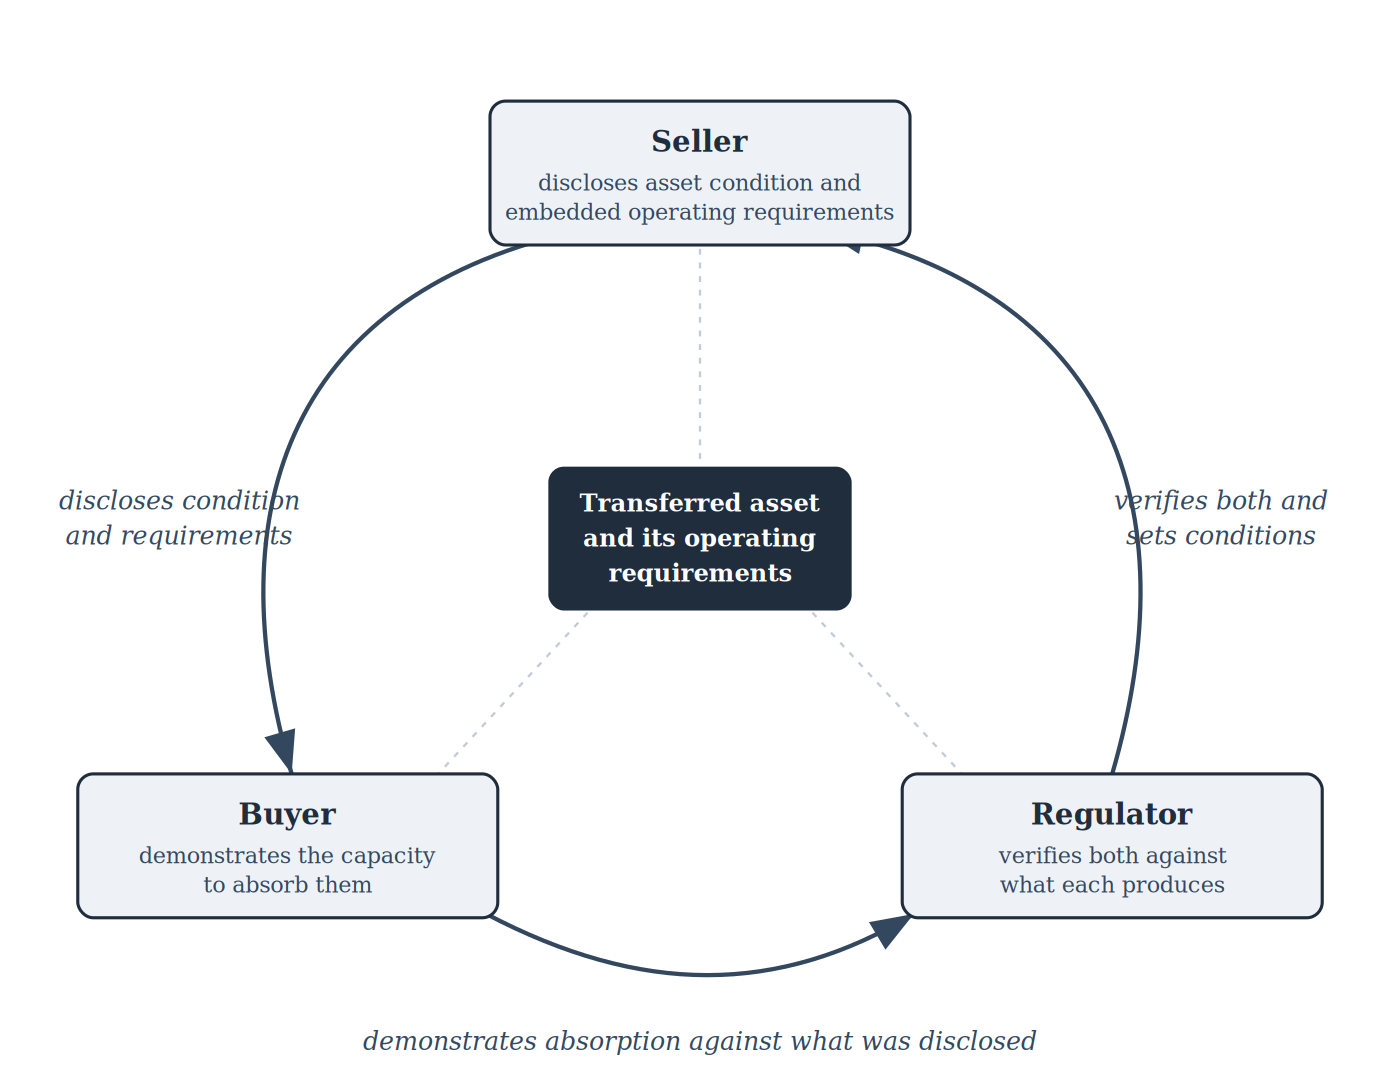
\includegraphics[width=\textwidth,height=0.45\textheight,keepaspectratio]{Figure_5_1_capability_assurance_loop.png}
\caption[The capability assurance loop]{The capability assurance loop. Seller disclosure, buyer absorption, and regulator verification act as three mutually constraining roles around the transferred asset. Weakness in any one role breaks the assurance, because the next role is left with nothing to act on.}
\end{figure}

That is the structure of the loop, which role acts on what. Its dynamics
are the complement: the same three roles are three balancing
interventions on the degrading cycle of Figure 2.1. Mandatory seller
disclosure closes the information gap at the point of sale; buyer
absorption verification confirms the capability before handover; and the
regulator's verification mandate, with rule-based triggers, installs the
requirement and restores the corrective signal the market does not send.
Each intervention cuts a different link, and the degrading cycle is
broken only when all three act together: a single intervention is
unlikely to close it, which is why disclosure without verification, or
verification without a buyer able to absorb, does not hold. Figure 5.2
places the three interventions on the same loop. Across the thesis the
three figures form one sequence: Figure 2.1 sets out the failure
equilibrium, Figure 5.1 the capability assurance loop that would close
it, and Figure 5.2 the points at which the framework cuts that loop.

\begin{figure}[H]
\centering
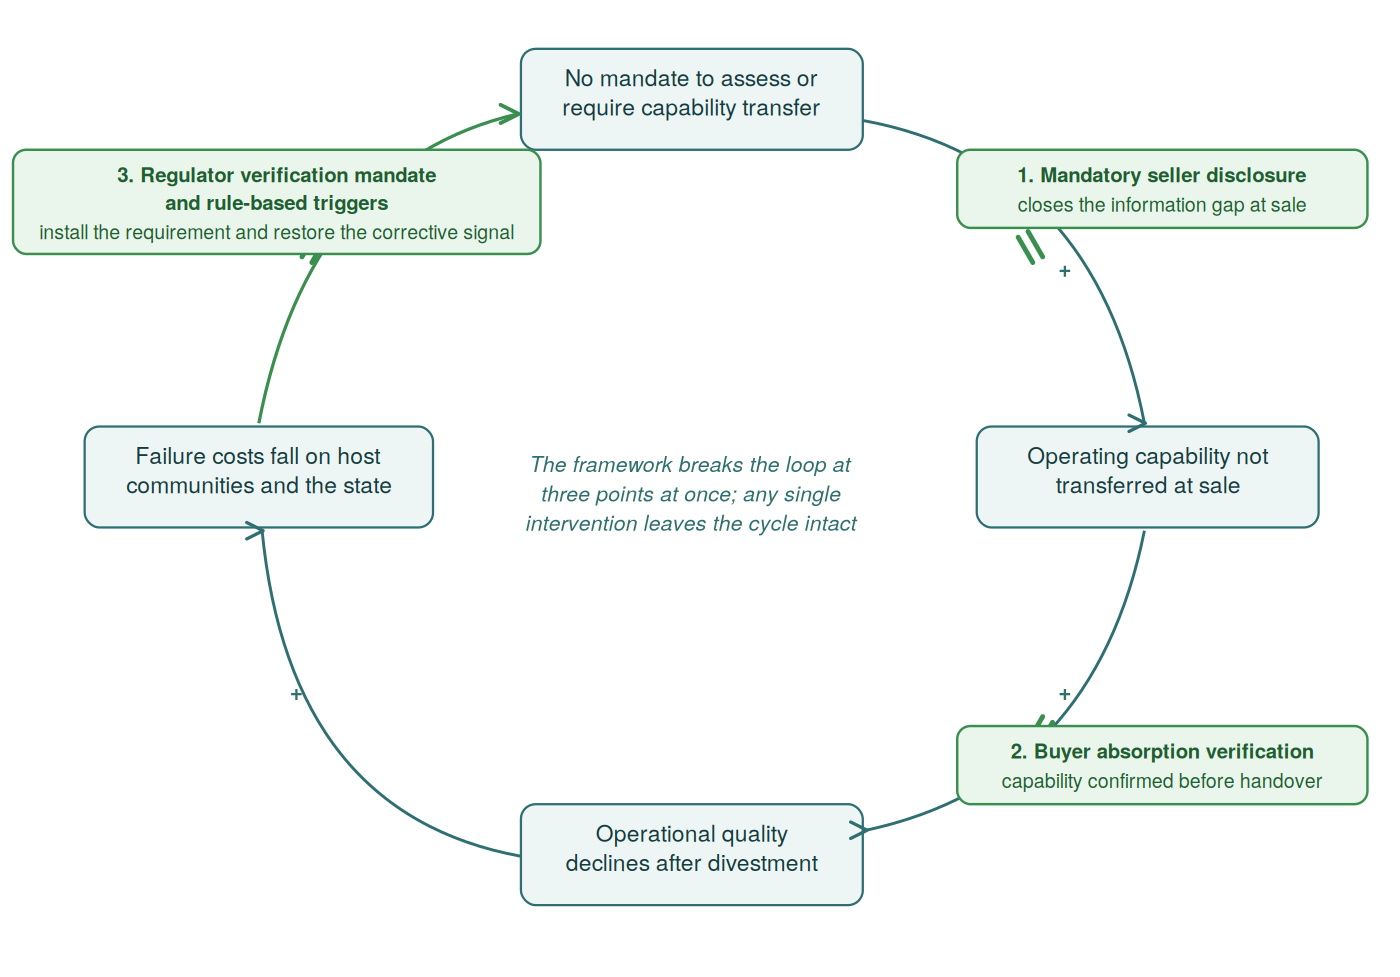
\includegraphics[width=\textwidth,height=0.45\textheight,keepaspectratio]{Figure_5_2_breaking_the_failure_equilibrium.png}
\caption[Breaking the failure equilibrium]{Breaking the failure equilibrium. The degrading cycle of Figure 2.1, with the framework's three roles acting as balancing interventions on different links. The loop is broken only when all three act together; any single intervention leaves the cycle intact.}
\end{figure}

\hypertarget{where-each-obligation-attaches-across-the-transaction}{%
\subsection{Where Each Obligation Attaches Across the
Transaction}\label{where-each-obligation-attaches-across-the-transaction}}

The three roles act at different points, and the points follow the order
in which knowledge actually moves between operators: before the
transfer, during it, and after close (Ferreira et al., 2024). Five
phases organize the obligations, two before the transfer commits, two
through the transition, and one after close.

Diagnosis comes first, before a buyer is committed. The seller discloses
the asset's condition and its embedded operating requirements, the
integrity and incident history, the status of wells including any that
are suspended or undecommissioned, and the catalogue of facilities and
their state. This extends the due diligence the Assignment of Interest
Regulations already require (Reg. 7) and the asset register that should
accompany it, and it reaches the information a buyer cannot recover from
a data room on its own. The case for it is direct: Aiteo inherited a
suspended well at Santa Barbara, and the reviewed record does not show
that its condition became an approval condition, a readiness test, or a
verified handover obligation (Section 4.3.1).

Transfer design follows, and it carries the most weight. The assignment
and transfer agreement sets out what moves with the asset and what
support the seller provides through the handover. These cover the
retention or secondment of operating staff, the transfer of data and
process knowledge, and a defined understudy period in which the buyer's
people work alongside those who hold the asset's operating knowledge.
These terms are mandatory in the design and beyond negotiation, because
they are the elements a buyer cannot supply for itself after close, and
the transfer-process evidence places them in its most-critical tier
(Appendix G, criticality tiers). Nigeria's content law already
contemplates this support in its succession and technology-transfer
provisions (NOGICD Section 31; Sections 43-47), written for a single
operator's workforce; the design binds them to the operatorship handover
itself. The contract is the instrument for two reasons. The
transfer-process evidence places contractual terms at the center of
whether knowledge moves, reaching more operating elements than any other
single factor (Ferreira et al., 2026). The operators that sustained
performance had retained, brought, or contracted equivalent operating
capability before performance depended on it (Sections 4.5.1 and 4.5.2).

Readiness is tested during the transition, before operatorship passes.
The buyer demonstrates that it can run this asset, not that it is
competent in the abstract: a working well-control response capability, a
safety-critical integrity backlog brought to a defined state, and an
understudy handover completed rather than promised. The competency
assessment can include the site visit the Regulations already permit
(Reg. 7). What justifies it is the gap between paper and practice: a
study of indigenous operating capacity found that firms passing a
table-top assessment failed when their facilities were inspected (Oriaku
et al., 2016). Aiteo's unreadiness was visible in the suspended well it
had not addressed.

Verification closes the transaction. The regulator confirms the
disclosed condition against the demonstrated capability and attaches
conditions to consent where a gap remains, including financial security
for decommissioning and for suspended wells (PIA Section 95; Sections
232-233). The contrast between two consents shows why: the regulator
withheld approval of the SPDC divestment to Renaissance until it was
satisfied on capability. The earlier transfer of OML 26 to a buyer whose
backers were later convicted of fraud passed under the prior regime
(Section 4.4.2).

Enforcement continues after close. The regulator monitors the indicators
that show whether capability held, for a defined initial period and then
on a trigger basis. It combines leading measures that signal readiness
before harm, drill completion, integrity-backlog closure, suspended-well
monitoring, and audit close-out, with the lagging process-safety event
rates that confirm it only once an incident has occurred. Where
readiness is incomplete at close, operatorship can be staged instead of
transferred whole, for instance through a phased transfer of operational
responsibilities across the transition, with the detailed options left
to Section 5.6. The financial security that backs decommissioning
liability follows the principle Alberta applies, held within the
existing Nigerian powers (PIA Sections 232-233; Section 95) rather than
imported as foreign law. Monitoring earns its place because
differentiated outcomes are observable only if they are measured, and
the cost of an unmeasured failure falls on the communities and the state
(Section 5.3.4).

The seller's duty in this design is bounded. It is to disclose fully and
to support the transition for a defined period, typically measured in
months, bounded well inside the life of the asset. Beyond that window,
the seller is not held liable for the buyer's operation.

The obligations are not uniform in weight. The disclosures and transfer
terms that only the seller can provide, and that the buyer cannot remedy
after close, sit in the most-critical tier of the transfer-process
evidence (Appendix G, criticality tiers), and these the design makes
mandatory. Obligations the buyer can manage are scaled to the risk of
the asset and the buyer, as developed in Section 5.6.

\hypertarget{the-bundle-by-capability-domain}{%
\subsection{The Bundle, by Capability
Domain}\label{the-bundle-by-capability-domain}}

The bundle is organized in Table 5.3 by the capability domains defined
in Section 5.2: the production and subsurface capability that sustains
output, and the four process-safety pillars that sustain integrity. Each
domain is paired with the corresponding seller, buyer, and regulator
obligations, with the empirical finding and the legal hook that warrant
it.

The cases populate the columns. On the seller side, the inherited
undecommissioned well, the absent blowout contingency plan, and the
facility catalogue the divestment did not produce are what a disclosure
obligation would have surfaced. On the buyer side, the operators that
absorbed capability show what the column asks for. They are Seplat under
Austin Avuru with Maurel et Prom, OML 30 under HEOSL with Salvic as
technical operator, and the SPDC divestment to Renaissance, designed to
preserve the operating capabilities, management systems, and staff of
the outgoing operator. Renaissance is evidence that
capability-preserving design is feasible and already emerging in
practice; it is not yet evidence of outcome, because the transfer is
recent. On the regulator side, the contrast between the decision to
withhold the Renaissance consent until capability was satisfied and the
earlier consent to a buyer it had no tool to test is what the
verification column is built from. The column also draws on the finding
that the response to the Aiteo blowout exceeded the operator's internal
capacity.

\begin{landscape}
\footnotesize
\begin{longtable}[]{@{}
  >{\RaggedRight\arraybackslash}p{(\columnwidth - 8\tabcolsep) * \real{0.2000}}
  >{\RaggedRight\arraybackslash}p{(\columnwidth - 8\tabcolsep) * \real{0.2000}}
  >{\RaggedRight\arraybackslash}p{(\columnwidth - 8\tabcolsep) * \real{0.2000}}
  >{\RaggedRight\arraybackslash}p{(\columnwidth - 8\tabcolsep) * \real{0.2000}}
  >{\RaggedRight\arraybackslash}p{(\columnwidth - 8\tabcolsep) * \real{0.2000}}@{}}
\caption[The capability bundle by domain: what is disclosed, absorbed, and verified]{The capability bundle: what the seller discloses, the buyer absorbs, and the regulator verifies, by capability domain. Each row carries the empirical finding and the legal hook that warrant it; the full element-by-element trace is in Appendix G.}\\
\toprule\noalign{}
\begin{minipage}[b]{\linewidth}\RaggedRight
Capability domain
\end{minipage} & \begin{minipage}[b]{\linewidth}\RaggedRight
Seller discloses
\end{minipage} & \begin{minipage}[b]{\linewidth}\RaggedRight
Buyer absorbs
\end{minipage} & \begin{minipage}[b]{\linewidth}\RaggedRight
Regulator verifies
\end{minipage} & \begin{minipage}[b]{\linewidth}\RaggedRight
Warrant: empirical finding and legal hook
\end{minipage} \\
\midrule\noalign{}
\endfirsthead
\toprule\noalign{}
\begin{minipage}[b]{\linewidth}\RaggedRight
Capability domain
\end{minipage} & \begin{minipage}[b]{\linewidth}\RaggedRight
Seller discloses
\end{minipage} & \begin{minipage}[b]{\linewidth}\RaggedRight
Buyer absorbs
\end{minipage} & \begin{minipage}[b]{\linewidth}\RaggedRight
Regulator verifies
\end{minipage} & \begin{minipage}[b]{\linewidth}\RaggedRight
Warrant: empirical finding and legal hook
\end{minipage} \\
\midrule\noalign{}
\endhead
\bottomrule\noalign{}
\endlastfoot
Production and subsurface operating capability & Reservoir and
production history, subsurface models, intervention and decline records
& Subsurface and production-operations competence, through a retained or
equivalent team & Demonstrated production-operations readiness, and
post-transfer production stability against the pre-transfer baseline,
with theft and sabotage distinguished from operator performance &
Absorbed operators sustained output where de novo operators did not
(Section 4.5); Reg. 7(a) and 7(g); pillar 7 \\
Commit to Process Safety (Pillar 1) & Safety management system,
competency records, workforce-retention plan & Safety culture and
competency, through retained staff and an understudy period & Corporate
competency and director fitness, and the team-retention plan & Aiteo's
downstream-only leadership against Avuru and Salvic's upstream pedigree
(Sections 4.5.1-4.5.2); NOGICD Sections 29-31; Reg. 7(5) \\
Understand Hazards and Risks (Pillar 2) & Process knowledge, hazard
analyses, asset data and databases & Process-knowledge management,
through retained data and the people who held it & Data repatriation
complete, hazard analyses current, and the asset's crisis scenarios
analyzed & The buyer could not assess embedded requirements from the
data room (Section 4.3.3); Reg. 7(g); NOGICD Sections 43-47 \\
Manage Risk (Pillar 3) & Operating procedures, integrity and maintenance
records and backlogs, emergency plans, well status, contractor
arrangements & Operating procedures, integrity management,
emergency-response capability, contractor architecture & Asset-specific
crisis readiness, a standing well-control arrangement, the integrity
backlog, and security for suspended wells & Aiteo well-control readiness
evidence: no contingency plan, no standing well-control contract,
after-the-fact specialist engagement, and an undecommissioned well
(Section 4.3.1, Section 4.3.6); Reg. 7(d); PIA Sections 232-233; pillar
4 \\
Learn from Experience (Pillar 4) & Incident history, prior
investigations, lessons learned, metrics & Incident-investigation
capability against the inherited history, and the metrics & Post-close
verification, leading indicators (drills, backlog closure,
suspended-well monitoring, audit close-out) and lagging process-safety
event rates & Capability is observable only if measured; table-top
assessment passed firms that site inspection failed (Oriaku et al.,
2016); Reg. 7(4); IOGP Report 456 \\
\end{longtable}
\end{landscape}

Footnote (below the table): In each row, the seller-disclosure and
transfer-agreement obligations are mandatory: they are the elements the
buyer cannot remedy after close, and they fall in the most-critical tier
of the transfer-process evidence (Appendix G, criticality tiers). The
buyer-absorption obligations are scaled to the risk of the asset and the
buyer (Section 5.6).

\hypertarget{calibration-existing-nigerian-rules-and-international-models}{%
\section{Calibration: Existing Nigerian Rules and International
Models}\label{calibration-existing-nigerian-rules-and-international-models}}

The design has precedent on both sides. NUPRC's 2024 reforms already
move in its direction, and the comparator regimes reviewed below require
a buyer to show capability, fitness, or organizational capacity before
they permit entry or a transfer. Where it goes beyond them is in
seller-to-buyer continuity of operating knowledge, and in verification
after close. Both points are established below, and from them follows a
specification of the buyer's own technical organization, which the next
section develops alongside the proportionality that scales it.

\hypertarget{the-domestic-foundation}{%
\subsection{The Domestic Foundation}\label{the-domestic-foundation}}

NUPRC's 2024 reforms moved in the right direction, and the design here
extends them, building on those reforms. The Nigeria Upstream Petroleum
(Assignment of Interest) Regulations 2024 already require due diligence
across technical capacity, financial capacity, decommissioning,
host-community and environmental funds, labor relations, and data
repatriation, and they permit site visits for competency evaluation
(NUPRC Reg. 7). The reviewed pre-2024 consent regime did not require the
operating-capability demonstrations the cases turn on: no blowout
contingency review, no well-control demonstration, no HSE
management-system assessment, no crisis-response or knowledge-transfer
requirement. The 2024 pillars reach adjacent concerns directly and some
operating-capability concerns indirectly, and the decommissioning escrow
secured under them, more than US\$400 million in 2024, is real progress
(NUPRC, 2024).

Specification and closure are achieved at four points. Reg. 7's
technical capacity, assessed largely at the corporate level, becomes a
demonstration of asset-specific operating capability tied to the
particular asset transferred. The discretionary competency visit becomes
mandatory and asset-specific for higher-risk transfers. Data
repatriation extends from a transfer of records into a structured
disclosure of asset condition and operating history. And a
seller-to-buyer transfer obligation and post-transfer verification,
absent from the pillars, are added, applying the logic of NOGICD's
succession and technology-transfer provisions, written for a single
operator's workforce, to the operatorship handover itself (NOGICD
Sections 31, 43-47).

\hypertarget{demonstrated-capability-in-international-practice}{%
\subsection{Demonstrated Capability in International
Practice}\label{demonstrated-capability-in-international-practice}}

Three comparator petroleum regulators assess operating capability before
they permit a transfer, and all three require evidence beyond
self-declaration, though they differ in how directly they test
operational capability. The claim is narrow and comparative: requiring a
buyer to show it can run an asset is not a novel demand in petroleum
regulation.

The United Kingdom's North Sea Transition Authority requires the buyer
and seller to prepare a capability pack, setting out the buyer's
financial and technical capability, before it consents to a license
assignment. It also assesses the fitness of a licensee and of those who
control it, including the incoming directors, whenever a licensee takes
on a new commitment. It holds a standing power to require a change of
control, or to revoke a license, where control passes to an unfit holder
(NSTA, 2023). Fitness, in the UK system, is a continuing criterion
rather than a one-time check.

Norway is more demanding on organization. A company cannot hold a
license or operate on the Norwegian continental shelf until it is
prequalified. Prequalification requires it to document technical
petroleum competence, health and safety competence, and financial
strength, assessed jointly by the Norwegian Offshore Directorate and
Havtil through meetings and site visits (Havtil. Norwegian Offshore
Directorate). The Petroleum Act requires a competent organization inside
Norway: licensees must keep technical staff in the country able to
follow the activity. Operators must maintain an in-country organization
capable of discharging the operator's duties, a materially higher bar
than the one set for a licensee (Norwegian Petroleum Act). Capability is
assessed at entry and supervised continuously after it.

Alberta assesses both parties to a transfer before it approves one.
Under the Licensee Life-Cycle Management framework introduced in 2021,
the regulator runs a multifactor licensee capability assessment that
weighs financial health, liability, and closure performance, and uses it
to decide eligibility to hold a license and the security required on a
transfer (AER, Directive 088). The framework ties the security a
transferee must post to that assessment and sets mandatory closure-spend
targets, keeping decommissioning capacity in step with the liability a
licensee carries.

These three regimes differ in emphasis, and each is built for its own
setting. None, as reviewed here, combines asset-specific
crisis-readiness verification for the particular asset, an obligation to
provide for continuity of operating knowledge through retention,
secondment, transition services, or equivalent technical support, and
post-transfer verification, in the form the Nigerian cases require. They
assess a buyer's corporate and financial capability, and Norway and
Alberta supervise it over time, but the combination Nigerian conditions
call for is not found in any one of them. The comparison, and what the
framework draws from each regime and adds beyond them, is set out in
Table 5.4.

\begin{longtable}[]{@{}
  >{\RaggedRight\arraybackslash}p{(\columnwidth - 6\tabcolsep) * \real{0.2500}}
  >{\RaggedRight\arraybackslash}p{(\columnwidth - 6\tabcolsep) * \real{0.2500}}
  >{\RaggedRight\arraybackslash}p{(\columnwidth - 6\tabcolsep) * \real{0.2500}}
  >{\RaggedRight\arraybackslash}p{(\columnwidth - 6\tabcolsep) * \real{0.2500}}@{}}
\caption[Capability as a condition of transfer across four petroleum regimes]{Capability assessment as a condition of transfer across four petroleum regimes, and what the proposed framework draws from them and adds. Every regime assesses a buyer's capability before transfer; the framework extends that practice by requiring asset-specific operating and crisis readiness, seller-to-buyer continuity of operating knowledge, and verification after transfer, none of which the comparators require.}\\
\toprule\noalign{}
\begin{minipage}[b]{\linewidth}\RaggedRight
Regime
\end{minipage} & \begin{minipage}[b]{\linewidth}\RaggedRight
Capability assessed before transfer
\end{minipage} & \begin{minipage}[b]{\linewidth}\RaggedRight
Form of the assessment
\end{minipage} & \begin{minipage}[b]{\linewidth}\RaggedRight
Continuing after transfer
\end{minipage} \\
\midrule\noalign{}
\endfirsthead
\toprule\noalign{}
\begin{minipage}[b]{\linewidth}\RaggedRight
Regime
\end{minipage} & \begin{minipage}[b]{\linewidth}\RaggedRight
Capability assessed before transfer
\end{minipage} & \begin{minipage}[b]{\linewidth}\RaggedRight
Form of the assessment
\end{minipage} & \begin{minipage}[b]{\linewidth}\RaggedRight
Continuing after transfer
\end{minipage} \\
\midrule\noalign{}
\endhead
\bottomrule\noalign{}
\endlastfoot
NUPRC, Nigeria (2024) & Seven-pillar due diligence: corporate technical
capacity, financials, decommissioning, host-community and environmental
funds, labor, data repatriation (Reg. 7) & Documentary; competency site
visit permitted but discretionary & Decommissioning escrow; no mandatory
post-transfer asset-specific operating-capability verification \\
United Kingdom (NSTA) & Buyer's financial and technical capability via a
capability pack; fitness of directors and controllers & Documentary
capability pack plus a fitness assessment & Fitness a standing
criterion; power to require a change of control or revoke \\
Norway (NOD and Havtil) & Prequalification for technical, HSE, and
financial competence; a competent in-country organization & Joint
meetings and site visits & Continuous supervision; in-country
organization maintained \\
Alberta (AER) & Multifactor licensee capability assessment of financial
health, liability, and closure performance (Directive 088) & Assessment
of the transferee's record and finances & Lifecycle monitoring; security
tied to liability; mandatory closure-spend targets \\
Proposed framework (Nigeria) & Asset-specific operating and crisis
readiness for the particular asset; seller-to-buyer continuity of
operating knowledge; buyer absorptive capacity & Mandatory
asset-specific demonstration and site verification for higher-risk
transfers & Leading and lagging integrity verification after transfer \\
\end{longtable}

\hypertarget{the-limits-of-voluntary-standards}{%
\subsection{The Limits of Voluntary
Standards}\label{the-limits-of-voluntary-standards}}

The technical content of operating capability is already codified. The
International Association of Oil and Gas Producers and IPIECA publish an
operating-management-system framework (IOGP Reports 510 and 511),
asset-integrity guidance (IOGP Report 415), and process-safety
performance indicators (IOGP Report 456) that describe, in detail, what
a competent operator does. The gap is not the content; it is the
delivery. These standards are voluntary, internal to a single operator,
and silent on the moment of transfer, and their adoption depends on the
buyer, including the buyers whose capability is the very thing in
question. That gap is closed by mandating through existing hooks what
the standards recommend, by naming them as the buyer's
integrity-management benchmark, and by using their process-safety event
rates, the Tier 1 and Tier 2 indicators, as lagging post-transfer
metrics. These are paired with leading indicators that signal readiness
before harm: readiness-drill completion, well-control-contract status,
integrity-backlog closure, suspended-well monitoring,
management-of-change compliance, near-miss reporting quality, and audit
close-out. A voluntary standard becomes an enforceable condition only
when a regulator attaches it to consent.

The calibration is therefore two-sided. The gate installed here has
precedent in Nigerian law and in the comparator regimes, and where it
reaches further, into seller-to-buyer transfer and post-transfer
verification, it does so to close a gap those regimes leave open. The
comparator models also specify what the buyer's own organization must
look like, an accountable operating entity, an inspectable in-country
organization, fit controllers, and a qualified technical operator where
in-house depth is absent. Those requirements are developed in Section
5.6, together with the proportionality that scales them to the asset and
the buyer.

\hypertarget{proportionality-and-structural-levers}{%
\section{Proportionality and Structural
Levers}\label{proportionality-and-structural-levers}}

A uniform requirement would be the wrong design. What is asked of a
buyer scales with two variables: the hazard the asset presents and the
operating capability the buyer brings to it. A buyer with demonstrated
comparable capability acquiring a low-hazard asset needs little beyond
confirmation of what it already holds; a de novo buyer acquiring an
asset with suspended wells, an evacuation dependency, and dense
community exposure needs the full apparatus. The cross-case evidence
defines the variables, and the obligations fall most heavily where the
process-safety criticality is greatest (Ferreira et al., 2026). The
requirements enforced at the gate, the risk tiers that scale them, and
the structural levers that carry them into a transaction are set out
below.

\hypertarget{requirements-for-the-buyers-organization}{%
\subsection{Requirements for the Buyer's
Organization}\label{requirements-for-the-buyers-organization}}

The comparator regimes do more than assess capability elsewhere; they
provide a template for an acquirer's operating organization, and the
case evidence populates it. Four requirements follow, and their
intensity scales with the asset's hazard and the buyer's profile in the
way the next subsection sets out.

The first is demonstrated upstream operating competence. The accountable
operating entity, whether through its own leadership or an approved
technical operator, must hold subsurface, operations, and
well-engineering experience on comparable assets, with named operational
accountability and the authority to command a well-control crisis. This
re-specifies Reg. 7(5)'s requirement of sufficient technical knowledge
and experience as asset-relevant operating depth in the entity that runs
the asset, not general managerial or commercial standing. The failure it
targets is the Aiteo containment failure, where the
leadership-background evidence pointed to downstream trading in place of
comparable upstream operating depth for directing a well-control
response (Sections 4.3.1, 4.5.1, and 4.5.2; Table 4.6). Leadership
background is a mechanism-consistency indicator rather than a proof of
cause, but the requirement follows from the absorptive-capacity argument
in any case: a firm cannot absorb operating knowledge it has no prior
expertise to receive (Cohen and Levinthal, 1990).

The second is an inspectable, accountable operating organization. The
buyer must run the asset through a real operating organization a
regulator can inspect, rather than a thin holding structure whose
operational depth cannot be independently demonstrated. The depth this
requires scales with asset risk, on the Norwegian
in-country-organization model at the high end, as the next subsection
sets out. The failure it targets is First Hydrocarbon Nigeria, a holding
vehicle that took an interest it never operated, leaving no operating
organization a regulator could have inspected (Section 4.4.2).

The third is controller fitness beyond a clean record. Reg. 7(5) screens
directors for prior convictions, which closes the narrow opening a
single prior conviction would present but not the wider one. The fitness
test should reach whether those who control the licensee can provide,
govern, and resource the technical and managerial capability the asset
requires, on the North Sea Transition Authority's model, drawing on the
fit-and-proper and disqualification provisions the PIA already contains.
The failure it targets is the governance collapse behind First
Hydrocarbon, whose principals were convicted of fraud committed while
leading the company. The point is not that the fraud would necessarily
have been discovered at approval, but that the earlier framework made
neither buyer fitness nor governance integrity a structured approval
question (Section 4.4.2).

The fourth is a technical operator or partner where in-house depth is
absent. A de novo buyer without operating depth of its own must supply
it through a qualified technical operator or a partnering arrangement,
the route the OML 30 operator took through Salvic and Seplat reinforced
through Maurel et Prom (Sections 4.5.1, 4.5.2). The failure it targets
is the de novo operator that runs a high-risk asset with neither
in-house depth nor a technical operator engaged, as at Aiteo. NOGICD's
technology-transfer and partnering provisions already contemplate the
arrangement (NOGICD Sections 43-47); whether it is mandatory or optional
is the proportionality question the next subsection answers.

\hypertarget{scaling-requirements-to-risk}{%
\subsection{Scaling Requirements to
Risk}\label{scaling-requirements-to-risk}}

The four requirements describe a ceiling, not a uniform floor, and three
variables set where a given transaction falls beneath it. The first is
the buyer's profile, read as demonstrated capability over corporate age
or size: a buyer that has run comparable assets carries capability into
the transaction, while a de novo buyer carries none and must build or
contract it. The second is the asset's hazard. Suspended wells that
require active integrity management, a single evacuation route whose
failure strands production, and proximity to populated communities each
raise the cost of an operating lapse, as the records of OML 29 and OML
18 show (Sections 4.3, 4.4). The third is the seller-transition
structure: a handover that retains the operating team and transfers the
management system presents a lower absorption risk than an abrupt exit
that strips both.

One part of the apparatus does not scale. The seller's disclosure, the
transfer of data and records, and a time-bounded mechanism for
continuity of operating knowledge are mandatory at every tier, because
they address failures a buyer cannot remedy on its own once the seller
has gone. The criticality finding identifies them as the most
safety-consequential of the transfer elements (Ferreira et al., 2026).
The transfer agreement is the instrument that carries them, and it must
specify the data and records to be transferred, the continuity
mechanism, and the transition period. What scales is the buyer-facing
burden: the depth of capability demonstration, whether a technical
operator is mandatory, the form the continuity mechanism takes, and the
intensity of post-transfer verification. The three tiers, and what each
requires, are set out in Table 5.5; the mandatory floor in the final row
applies in addition to every tier above it.

\begin{landscape}
\footnotesize
\begin{longtable}[]{@{}
  >{\RaggedRight\arraybackslash}p{(\columnwidth - 8\tabcolsep) * \real{0.2000}}
  >{\RaggedRight\arraybackslash}p{(\columnwidth - 8\tabcolsep) * \real{0.2000}}
  >{\RaggedRight\arraybackslash}p{(\columnwidth - 8\tabcolsep) * \real{0.2000}}
  >{\RaggedRight\arraybackslash}p{(\columnwidth - 8\tabcolsep) * \real{0.2000}}
  >{\RaggedRight\arraybackslash}p{(\columnwidth - 8\tabcolsep) * \real{0.2000}}@{}}
\caption[Risk-tiered divestment assurance scaled to demonstrated capability]{Risk-tiered divestment assurance. The apparatus required of a buyer scales with the capability it demonstrably brings, read independently of corporate age, and with the hazard the asset presents; the mandatory floor in the final row applies at every tier, since it addresses failures a buyer cannot remedy after transfer. In the retrospective examples, the cases examined are classified under the framework, which did not exist at the time of those transactions.}\\
\toprule\noalign{}
\begin{minipage}[b]{\linewidth}\RaggedRight
Tier
\end{minipage} & \begin{minipage}[b]{\linewidth}\RaggedRight
Retrospective example
\end{minipage} & \begin{minipage}[b]{\linewidth}\RaggedRight
When it applies
\end{minipage} & \begin{minipage}[b]{\linewidth}\RaggedRight
Required of the buyer
\end{minipage} & \begin{minipage}[b]{\linewidth}\RaggedRight
Transfer and verification apparatus
\end{minipage} \\
\midrule\noalign{}
\endfirsthead
\toprule\noalign{}
\begin{minipage}[b]{\linewidth}\RaggedRight
Tier
\end{minipage} & \begin{minipage}[b]{\linewidth}\RaggedRight
Retrospective example
\end{minipage} & \begin{minipage}[b]{\linewidth}\RaggedRight
When it applies
\end{minipage} & \begin{minipage}[b]{\linewidth}\RaggedRight
Required of the buyer
\end{minipage} & \begin{minipage}[b]{\linewidth}\RaggedRight
Transfer and verification apparatus
\end{minipage} \\
\midrule\noalign{}
\endhead
\bottomrule\noalign{}
\endlastfoot
Tier 1 (full) & Aiteo (OML 29); OML 30 & A de novo buyer, or a buyer
without demonstrated comparable capability acquiring a high-hazard asset
& All four requirements; a qualified technical operator or partner is
mandatory & Full-form continuity mechanism; staged operatorship on
demonstrated readiness; financial security tied to decommissioning;
leading and lagging integrity triggers; community-readiness measures
where exposure is dense \\
Tier 2 (intermediate) & Seplat (OMLs 4, 38, 41) & A buyer with
demonstrated comparable capability acquiring a moderate-to-high-hazard
asset & Operating competence, inspectable organization, and controller
fitness demonstrated; technical operator at the regulator's discretion &
Continuity mechanism scaled to need; integrity triggers; staged
operatorship at discretion \\
Tier 3 (baseline) & None in the present set & A buyer with demonstrated
comparable capability acquiring a low-hazard asset & Operating
competence and controller fitness confirmed & Documented handover;
standard post-transfer reporting \\
Mandatory floor (all tiers) & All transactions & Every transfer, in
addition to the requirements above & Receipt and integration of the
disclosed knowledge & Seller disclosure; data and records transfer; a
time-bounded continuity-of-knowledge mechanism, all specified in the
transfer agreement \\
\end{longtable}
\end{landscape}

The tiers track the cases in retrospect. Aiteo on OML 29 would classify
as Tier 1, a de novo buyer on a high-hazard asset, and the apparatus it
would have required, a mandatory technical operator and a demonstrated
containment capability, is what the record shows absent (Section 4.3).
The OML 30 transaction would classify as Tier 1 on the same reading, an
indigenous buyer without its own operating depth. It cleared the bar the
framework would set by supplying that depth through Salvic, which is why
its outcome diverged from Aiteo's under otherwise similar conditions
(Section 4.5.2). Seplat illustrates why the tiering turns on
demonstrated capability over corporate age: newly formed in 2010, it
brought upstream operating capability through its founding team and its
technical partnership with Maurel et Prom. It would fall within Tier 2
instead of carrying the full Tier 1 burden (Section 4.5.1).

\hypertarget{the-structural-levers}{%
\subsection{The Structural Levers}\label{the-structural-levers}}

Five levers carry the tiered requirements into the transaction, and each
rests on a case in the record and an existing legal hook.

The first is a mandated technical-operator or partnering arrangement for
de novo buyers at Tier 1. Where the buyer's own organization cannot
demonstrate operating depth, an approved technical operator must supply
it, the arrangement OML 30 used and Aiteo did not (Sections 4.3.1,
4.5.2). NOGICD's technology-transfer and partnering provisions supply
the statutory basis (NOGICD Sections 43-47).

The second is a time-bounded mechanism for continuity of operating
knowledge. Because people cannot be transferred like equipment, the
transfer agreement must provide a defined route by which the knowledge
that ran the asset reaches the buyer, through secondment, retention
incentives, transition-service arrangements, or guaranteed access to
named subject-matter experts. The arrangement must run for a period long
enough to transfer working knowledge and short enough not to leave the
seller indefinitely responsible for an asset it has sold. The
process-safety record supplies the warrant: incidents rose after
handovers that retained no operating team (Ferreira et al., 2026). The
Renaissance transaction is a design contrast that shows the arrangement
is structurable. Shell stated that the sale was designed to preserve
SPDC's operating capabilities, including its management systems, and
that its staff would continue to be employed through the change of
ownership (Shell, 2024). That transaction completed only in 2025, so it
offers feasibility evidence rather than validation of outcomes. NOGICD's
succession and understudy provisions, written for a single operator's
workforce, supply the closest statutory analogue (NOGICD Section 31).
The handover runs against a shared knowledge repository that both
parties review before transfer, the transfer instrument the
inter-organizational knowledge-transfer literature places at the center
of whether operating knowledge moves (Ferreira et al., 2024).

The third is staged operatorship, a phased assumption of operational
responsibility in which critical functions pass only after readiness is
demonstrated, instead of at a single administrative moment. This gives
the absorptive-capacity requirement a point of verification before full
responsibility passes (Cohen and Levinthal, 1990).

The fourth is financial security tied to decommissioning liability. The
buyer must post security scaled to the abandonment obligation it
assumes, the mechanism Alberta operates through its licensee assessment,
and the one the PIA and the 2024 escrow already begin to build in
Nigeria (AER, Directive 088; PIA Sections 232-233; NUPRC, 2024).

The fifth is a set of post-transfer integrity triggers, leading and
lagging. Lagging indicators, the IOGP Tier 1 and Tier 2 process-safety
event rates, register harm after it occurs. Leading indicators,
readiness-drill completion, integrity-backlog closure, suspended-well
monitoring, management-of-change compliance, near-miss reporting
quality, and audit close-out, signal a developing capability gap before
it produces an incident, which gives the closed loop a point of
intervention ahead of failure rather than only after it.

Indicators are only as strong as the consequences attached to them. The
triggers should connect to graduated, rule-based consequences applied on
defined thresholds, escalating conditions on operatorship and financial
consequences scaled to the breach, rather than to consequences that
depend solely on discretionary regulatory action. The NPDC case shows
why the distinction matters: where enforcement turns on discretion,
political access can deflect it (Section 4.5.3). Rule-based triggers
reduce, though they do not eliminate, that vulnerability, and they tie
the verification loop to the financial security the fourth lever
establishes. Where the asset carries dense community exposure, the
readiness test extends beyond the technical to a set of
community-readiness measures: host-community notification protocols,
spill-response interface arrangements, and linkage to the Host Community
Development Trust the PIA requires (PIA Chapter 3).

The obligations placed on the seller are those only the seller can
initiate: disclosure of asset knowledge, access to records and
subject-matter experts, and a time-bounded continuity mechanism. They
attach to the transaction and expire at the end of a defined transition,
short of extending the seller's liability for the asset indefinitely.

No framework can guarantee that a buyer which clears every tier will
succeed. What it offers instead is assurance in the proper sense: it
makes the capability an asset needs observable, testable, and
enforceable before and after the asset changes hands. The boundaries of
that assurance are the subject of Section 5.7.

\hypertarget{design-risks-and-the-limits-of-the-warrant}{%
\section{Design Risks and the Limits of the
Warrant}\label{design-risks-and-the-limits-of-the-warrant}}

The framework is warranted, not proven. It rests on the regularities
established across the cases and on the logical completeness of the
design that follows from them, not on a tested intervention; no
implementation data yet exists. What the design assures is capability
that can be observed, demonstrated, and verified; it does not reach the
non-contractible tacit knowledge no instrument can compel a seller to
surrender, and it does not guarantee outcomes. Its contribution is to
make the capability an asset needs observable and testable at the point
of transfer, not to ensure on its own that the capability is there. The
seller's obligations are deliberately time-bounded, a defined transition
in place of indefinite liability; after that window, responsibility for
operating the asset rests with the buyer, though the post-transfer
verification and enforcement remain in force.

The central confound is one the design tolerates rather than resolves.
The evidence did not cleanly separate whether an operator's difficulty
traced to the specific capability it inherited or to its general
organizational quality, and the two run together in the cases, as noted
in Section 4.8. The design does not hinge on the distinction. The same
assurance screen detects both, though the response it calls for differs:
a structured transfer of the seller's knowledge answers an
asset-specific gap, while technical-operator support or, in the limit,
refusal of consent answers a broader organizational one. The confound
limits the precision of the causal account in the case analysis; it does
not weaken the design, which detects a capability gap without needing to
attribute it to one source over the other.

Two further limits follow from the evidence base. The internal
coordination through which a firm absorbs operating capability was
inferred from outcomes and documents rather than observed directly. The
absorptive-capacity mechanism the design relies on is warranted by
theory and by the outcome pattern, not by direct observation of how each
organization worked inside. And the primary cases concentrate on a
single seller. The seller-independence checks bound the concern, since
an acquirer's capability gap can arise under any seller where buyer
absorption and regulatory verification are weak. The empirical base,
however, remains weighted toward one divesting company, and the
generalization to other sellers rests on the logic of the capability
argument more than on a balanced sample.

The framework can also misfire in implementation, and the most likely
way is the substitution of paper for practice. Its premise is
demonstrated capability, not a certificate attesting to it, and a
regulator that accepted documentary compliance in place of a
site-verified demonstration would reproduce the failure the design
exists to prevent. Norway's reliance on meetings and site visits, and
the finding that firms which passed a table-top assessment failed a
subsequent facility inspection, both warn that the demonstration must be
of the operating reality and not of the paperwork (Oriaku et al., 2016).
A deeper implementation risk is institutional capacity. The design asks
the regulator to verify capability on site, sustain post-transfer
monitoring, set and enforce conditions, and share evidence across
agencies, and it will not work where the regulator lacks the staff, the
data access, the independence, or the political backing to do so.
Regulatory inadequacy was an enabling condition of the failures (Chapter
4), so the framework presupposes a capacity whose weakness it must also
withstand. A second misfire runs the other way: a bar set too high
deters capable acquirers and narrows an already thin pool of credible
operators. The tiering is the instrument meant to hold the burden in
proportion to risk, but its boundaries are qualitative and left to
regulatory judgment, and if set too conservatively, the framework would
raise entry barriers without a commensurate gain in assurance. The
design is calibrated against under-protection and over-deterrence both,
and the balance between them falls to implementation rather than to
design alone.

The enforcement and verification mechanisms are specified in principle
rather than as worked schemes. The integrity triggers connect to
rule-based consequences, but who sets the thresholds, who administers
them, and at what levels are questions of institutional design left open
here. The rule-based direction addresses the political-economy
vulnerability documented in the case analysis, but it is not a finished
enforcement architecture. The same holds for the community-readiness
measure, whose force depends on the linkage a regulator builds between
it and the Trust structure the PIA already requires.

These limits are bounded by jurisdiction, and the boundary is not
uniform across the design, which operates at two levels. The general
level, the capability-assurance logic, the seller-disclosure obligation,
the absorptive-capacity requirement, and the regulator-verification
role, is calibrated to the institutional conditions that characterize
petroleum-producing developing countries. Those conditions are
constrained regulatory capacity, high externality exposure, and the
active transfer of producing assets from international to domestic
operators. The framework would carry to any divestment regime that
shares them. The specific level, the particular legal hooks and the
indigenous-operator framing, is tied to Nigeria, to the PIA, the NUPRC
regulations, and NOGICD, and to the operating environment of the Niger
Delta. The demonstration here is on upstream producing-asset transfers,
where integrity failures and their externalities are most acute. The
same logic extends to midstream and downstream transfers, which proceed
under Section 117 and the Authority instead of Section 95 and the
Commission, though that extension is not demonstrated by the cases
examined. Transfer to another setting or subsector would keep the logic
and re-fit the hooks, subject to local validation. The broader
implications and the directions for further research are taken up in the
conclusions.

\hypertarget{conclusions}{%
\chapter{Conclusions}\label{conclusions}}

The question was why the transfer of these assets from international to
indigenous operators produced such different results, and what should
follow from it. The answer is that capability-related factors best
account for the differences, which do not track the capital each
acquirer raised, the fiscal terms it faced, or the regulatory regime it
worked under. The gap that produces this divergence is built into the
structure of the transfer rather than into any single operator. What the
evidence warrants is a mandatory, asset-specific assurance mechanism for
high-risk producing-asset transfers.

Behind that answer is a particular way of seeing the asset. A producing
field is a sociotechnical system, the physical facilities and the
operating organization that runs them working as one, and a divestment
that conveys the facilities while leaving the organization behind
separates the system from the capability that kept it safe and
productive. In those terms, the cases reveal a control failure in how
the transfer is built, one whose cost falls largely outside the sale
(Figure 2.1). The framework developed in Chapter 5 is a control
structure designed to close that loop.

The answers to the research questions come first (Section 6.1), followed
by why the gap calls for a mandatory rather than a voluntary response
(Section 6.2). The recommendations that follow from it are set out next
(Section 6.3), then the limits of the findings (Section 6.4) and the
boundaries of their generalizability (Section 6.5). The contribution is
stated last (Section 6.6).

\hypertarget{answering-the-research-questions}{%
\section{Answering the Research
Questions}\label{answering-the-research-questions}}

This thesis opened with three questions, and the case analysis answers
each (Chapter 4). First, the differentiated outcomes are most consistent
with capability-related factors: the acquirers separated according to
the operating capability each inherited, brought, contracted, or
embedded before performance depended on it. Second, the evidence
contradicts fiscal regime effects for these cases and rejects capital
constraints as sufficient for the funded operators, finds regulatory
inadequacy and political economy each enabling but insufficient on its
own. It leaves capability-related factors as the explanation most
consistent with the integrity outcomes. Third, because the explanation
is capability-related, the remedy is a three-actor Capability Assurance
Framework that makes operating capability observable, testable, and
enforceable at the point of transfer, with the seller disclosing
requirements, the buyer demonstrating absorption, and the regulator
verifying both.

Across the two outcome dimensions, production performance and
operational integrity, the acquirers did not converge: they separated
into distinct trajectory groups, and the separation lines up most
closely with the operating capability each acquirer inherited, brought,
contracted, or embedded before performance depended on it. The
separation does not track the capital each raised, the fiscal terms each
faced, or the regulatory regime each worked under.

Capital constraints, the common explanation, are rejected as sufficient.
On the OML 29 critical experiment, the operator that suffered the most
serious integrity failure had funded and delivered production growth
beforehand, and an operator able to raise and deploy capital for
production cannot have its later integrity failure explained by capital
scarcity alone. A separate body of evidence points to capability: no
standing well-control contract or matching contingency plan when the
Santa Barbara well blew out, specialist intervention engaged only after
the fact, and a suspended, undecommissioned well the operator was
unready to control. The pattern points to capability, with the national
spill agency recording that the event exceeded its internal capacity
(Section 4.3). The two readings rest on different evidence.

Regulatory inadequacy is an enabling condition, not the primary driver.
The test is differentiation: were a weak regime the cause, acquirers
under it would perform alike, yet under the same pre-2024 regime that
governed Aiteo, Seplat and the HEOSL operatorship sustained production
without an equivalent integrity failure (Section 4.5). A regime common
to all cannot explain outcomes that varied sharply among them; what it
does is let the consequences of a capability shortfall go uncaught: it
is the setting in which a capability shortfall produces harm, while the
shortfall itself originates in the transfer.

Fiscal regime effects are rejected on timing: every primary transaction,
and the capability gaps that produced the failures, predate the
Petroleum Industry Act of August 2021, and the divergence under
identical pre-Act terms reinforces the point; whether the Act shapes
future transactions is left open. Political economy explains which firms
acquired and kept operatorship, and the production gains that
connections secure by suppressing theft, but it does not reach the
case-level capability to sustain integrity or contain a well-control
crisis. Why two firms on comparable terms then diverged in whether they
could run their assets safely is a question it leaves open.

The within-asset comparison on OML 30 is the strongest evidence against
the obvious competing reading, that outcomes track asset quality.
Operatorship passed from NPDC to HEOSL on the same wells, reservoirs,
and facilities, and performance improved under the new operator, which
is hard to reconcile with an asset-quality account. The population-level
evidence, and the marginal-field program of 2003 to 2020 in which a
majority of licensed operators also failed to sustain their assets, are
consistent corroborating context that does not, by itself, carry the
verdicts.

The five explanations resolve as follows. Capital constraints are
rejected as sufficient; fiscal regime effects are rejected for the cases
examined, the transactions and capability gaps predating the PIA.
Regulatory inadequacy is an enabling condition, insufficient on its own.
Political economy accounts for commercial survival and continued
participation but is insufficient on its own for operational integrity.
Capability-related factors are most consistent with the combined
pattern, with the OML 30 comparison strengthening that reading against
an asset-quality explanation. That answers the first two research
questions and grounds the design argument that follows.

\hypertarget{the-structural-case-for-mandatory-intervention}{%
\section{The Structural Case for Mandatory
Intervention}\label{the-structural-case-for-mandatory-intervention}}

The differentiated outcomes are not reducible to individual
mismanagement, to be corrected one operator at a time. They follow from
how the transaction itself is built. At the point of divestment the
information about an asset's embedded operating capability sits with the
seller, the capacity to absorb that capability sits with the buyer, and
the full social cost of a capability shortfall falls on neither. The gap
is structural, a control failure in the design of the transfer, not a
defect peculiar to any one acquirer.

Three features of the transfer make it so, each set out in the economics
of the transaction (Section 2.5). Information asymmetry comes first. The
seller knows what its operating organization does to hold an aging asset
within safe bounds; a buyer cannot read that from a data room, and the
regulatory screen at consent does not reach the asset-specific
capability at issue. The party that knows the most about the embedded
capability has little incentive to surface it, since fuller disclosure
can lower the price, slow the close, or create transition obligations,
and the party that carries the operational risk cannot verify what it is
buying. Absorptive capacity is the second, and it sits on the buyer's
side. A seller willing to hand over everything it knows still cannot
make that knowledge land in an organization without the prior expertise
to receive and embed it. The capability has to be present before
performance depends on it, which is the line the cases divided along.
The third is the externality. When an operator cannot contain a
well-control event or sustain integrity, the cost falls on host
communities and on the Nigerian state, parties outside the sale and
absent from its terms.

These three features have one consequence in common. Voluntary transfer
cannot solve a problem whose critical information is held by the seller,
whose absorption depends on the buyer, and whose failure costs are borne
by communities and the state. Voluntary instruments do not escape it.
The industry's operating and process-safety standards and the
civil-society National Principles for Responsible Petroleum Industry
Divestment describe the right content, but they attach no consequence to
ignoring it and leave the underlying incentives untouched (Section
5.5.3). Each describes what a responsible transfer should look like.
None compels it.

The instruments that do carry legal force have a different weakness: the
ones meant to protect the exposed parties are funded out of the
operations that fail. The Host Communities Development Trust is funded
by a contribution equal to three percent of the operator's actual annual
operating expenditure (PIA Section 240). When an operator falters and
operations contract, that contribution contracts with them, leaving the
fund thinnest when the hazard is greatest. The decommissioning
obligation runs the same way from the other direction. Where the
Decommissioning and Abandonment Fund is left to accrue across the
producing life of the asset rather than secured at transfer (Sections
232 and 233), an operator that fails early has set aside only a fraction
of what closing its wells will cost. Both mechanisms are necessary, and
each delivers least when it is needed most.

The structure points to a single remedy, security taken at the front of
the transaction rather than left to accrue. The Act already provides an
analogous structure: its environmental remediation provision requires a
financial contribution the Commission can reach (Section 103), fixed at
the point of operation rather than dependent on the operator's later
solvency. Extending that logic to operating capability and to community
exposure is the work of the recommendation developed below. The deeper
reason the transaction cannot correct itself is that the parties who
bear the residual cost are not at the table. Host communities and the
state cannot bargain ex ante over terms they never see, so the
externality cannot be priced into a private deal and must be placed
there by the body that licenses the transfer.

The third research question asked what institutional design follows from
these findings, and how responsibility should be allocated across the
seller, the buyer, and the regulator. A voluntary framework would
suffice only if market forces or the existing rules already secured
capability transfer. They do not. Outcomes diverged sharply under a
common regulatory regime, the transacting parties hold neither the
information nor the incentive to close the gap on their own, and the
full social cost of failure falls outside the sale. The rules already in
force do not reach the asset-specific operating-capability question at
consent. The Commission's 2024 reforms created a technical-capacity
route, but it is assessed at the corporate level, and a corporate screen
can pass an operator that has not demonstrated the asset-specific crisis
readiness the cases show to be decisive. The provisions that reach past
consent are triggered by failure rather than preventing it. What the
evidence warrants is a mandatory, asset-specific assurance mechanism for
high-risk producing-asset transfers, the control structure designed to
close the severed loop (Figures 5.1 and 5.2), allocating disclosure,
demonstrated absorption, and verification across the seller, the buyer,
and the regulator.

\hypertarget{prioritized-recommendations}{%
\section{Prioritized
Recommendations}\label{prioritized-recommendations}}

The full framework, with its three roles, five lifecycle phases, and
risk tiers, is developed in Chapter 5. For implementation, six
recommendations follow from it, ordered from before consent to after
close, each re-specifying an instrument the Nigerian regime already
contains rather than adding a new one. They carry the framework's
disclosure floor and its five structural levers (Section 5.6.3) into
instrument form. Together they put the framework's three roles into
operation: what the seller must disclose, what the buyer must
demonstrate, and what the regulator must verify and enforce. They are
risk-tiered: a disclosure, data, and continuity floor applies to every
transfer, while staged operatorship, technical-operator coverage, and
intensified post-transfer verification apply to the highest-risk assets
and lowest-capability buyers. Disclosure and continuity come first,
because the recommendations that follow depend on them.

\begin{enumerate}
\def\labelenumi{\arabic{enumi}.}
\item
  A regulator approving the transfer of a high-risk producing asset
  should require, as a condition of consent, that the seller disclose
  the asset's condition and the operating requirements it imposes, and
  that the buyer demonstrate the operating capability and
  crisis-response readiness to meet them. This follows from the
  documented condition that the information determining whether an aging
  asset can be held within safe bounds sits with the seller and cannot
  be read from a data room. In Nigeria the requirement attaches to the
  ministerial consent already mandatory for assignment of an upstream
  license or lease (PIA Section 95) and to the due-diligence requirement
  under the Nigeria Upstream Petroleum (Assignment of Interest)
  Regulations 2024 (Reg. 7). It makes asset-specific disclosure and a
  demonstrated well-control and crisis-response capability explicit
  conditions of consent. Neither is left to the buyer's discretion after
  close. Aiteo's transfer closed with no documented well-control
  contingency for OML 29 and no standing well-control contract, the gap
  that surfaced in the Santa Barbara blowout (Section 4.3). A
  disclosure-and-readiness condition at consent is the point at which
  that gap is still visible and correctable.
\item
  The transfer should carry binding terms that keep an aging asset's
  operating knowledge available to the buyer through and beyond the
  handover. That knowledge holds the asset within safe bounds, and it
  resides in the people who hold it, the procedures that codify it, and
  the working practices through which it is applied. Hardware transfers
  at completion; the embedded operating knowledge does not, and tacit
  knowledge in particular leaves with its holders. Nigeria already
  requires a succession plan and a multi-year understudy of incumbent
  expertise under the Nigerian Oil and Gas Industry Content Development
  Act (NOGICD, Section 31). That mechanism was built for
  expatriate-to-Nigerian succession. Re-specified toward seller-to-buyer
  transfer at divestment, and written into the assignment agreement
  under Section 95 as binding terms for retention, secondment, data, and
  understudy rather than negotiated ones, it would function as an
  obligation to carry the operating knowledge across the change of
  hands. The HEOSL recovery on OML 30, where a technical operator held
  that knowledge through the transition, shows what such terms are meant
  to secure.
\item
  Consent should depend on the buyer demonstrating the organizational
  capacity to receive and embed the disclosed capability, not on
  financial and legal standing alone. Disclosed knowledge cannot land in
  an organization that lacks the prior expertise to absorb it, which is
  the line the cases divided along. This re-specifies the
  technical-capacity criterion already within the consent assessment
  (Section 95; Reg. 7), raising it from a corporate-level screen to an
  asset-specific demonstration. For Tier 1 assets, the highest-risk
  tier, the demonstration should normally include a qualified technical
  operator with a record on comparable operations, drawing on the
  technology-transfer and partnering route the content law already
  contemplates (NOGICD Sections 43-47). In Aiteo, the
  leadership-background evidence pointed to downstream trading rather
  than comparable upstream operating depth. Seplat brought that depth,
  through its founding team and its technical partnership with Maurel et
  Prom. That contrast is the case basis for testing absorptive capacity
  before consent, not discovering its absence after.
\item
  For high-risk transfers, operatorship should pass in stages rather
  than at a single completion date, with critical operating functions
  passing only after the buyer has demonstrated readiness for them.
  Time-bounded transition support, technical-operator coverage, or
  secondment holds the asset within safe bounds during the transition,
  without leaving the seller indefinitely responsible for an asset it
  has sold. An abrupt handover concentrates the capability discontinuity
  at the moment of greatest exposure, before the buyer has shown it can
  run the asset. In Nigeria staged operatorship is a condition the
  Commission can attach to consent under Section 95, supervised under
  its standing authority to monitor and enforce the terms of leases and
  licenses (Section 7(d)). It requires no new instrument. The phased
  technical-operator arrangement through which OML 30 was returned to
  stable operation is the design pattern. The single-date handover at
  Aiteo, into an organization without demonstrated upstream operating
  depth, is the failure that staged operatorship is built to prevent.
\item
  The regulator should verify operating capability on a continuing basis
  after transfer, prompted by rule-based triggers, production or
  integrity deviations, missed maintenance intervals, the loss of key
  operating personnel, rather than by discretion alone. A capability
  shortfall invisible at consent becomes visible only in operation, and
  an unmonitored latent exposure is the most dangerous kind. Nigeria's
  regulator already holds the powers this requires: to monitor and
  enforce compliance with the terms of leases and licenses (Section
  7(d)), and to carry out audits and investigations of licensees
  (Section 7(g)), with administrative penalties available for
  contravention (Section 231). Binding those powers to defined triggers
  connects an integrity finding to a graduated, pre-defined consequence
  rather than to discretion, subject to the operator's opportunity to
  respond. The powers already exist; the triggers are what is missing.
  The well left suspended and undecommissioned on OML 29 from 2015,
  unmonitored until it failed in 2021 (Section 4.3), is the exposure
  continuing verification is built to catch.
\item
  The financial security for decommissioning and for community exposure
  should be taken at the point of transfer rather than allowed to accrue
  out of the operations that may fail. An instrument funded from ongoing
  operations delivers least when the operator falters, which is the
  moment it is most needed. The remedy is to secure it at consent. The
  amount should scale to the asset's risk and inherited liabilities.
  This removes the dependency the existing instruments carry, the Host
  Communities Development Trust's three-percent-of-operating-expenditure
  base (Section 240) and the decommissioning fund's accrual across the
  producing life of the asset (Sections 232 and 233). It extends the
  upfront structure the Act already uses for the environmental
  remediation contribution (Section 103) to decommissioning security and
  community-readiness provisioning fixed at consent. The
  undecommissioned well on OML 29 and the 41 communities exposed by the
  blowout are the costs this provisioning is meant to cover before, not
  after, an operator's capacity to pay has eroded.
\end{enumerate}

The six divide by where they attach. Recommendations 1 through 4 attach
to the consent gate, the one-time approval at transfer. They therefore
apply only to transfers not yet completed, the divestments still to come
in a wave of IOC onshore exits that is not finished, and cannot be
re-run on a transaction already closed. The consent-stage screening they
require is not hypothetical: the Commission applied a version of it when
it initially withheld consent for the Shell-to-Renaissance transfer in
2024 on the ground that the consortium had not demonstrated the
requisite technical capacity. The Commission granted consent later that
year (The Energy Year, 2025; BusinessDay, 2025). Recommendations 5 and 6
attach to powers and obligations that bind every current operator
continuously: the Commission's standing supervisory powers (Sections
7(d) and 7(g)) and the standing fund obligations under Sections 232-233
and 103. They therefore reach the assets already transferred, Aiteo and
Eroton included. Applying them to current operators enforces standing
obligations rather than reopening closed consent decisions. It would not
re-run the original transfer; it would apply continuing powers and
standing obligations to operating risks that are still live. That is
where the exposure now sits.

None of this builds a second regulatory track alongside the one the
Commission introduced in 2024. That route assesses capacity at the
corporate level; the recommendations re-specify the same consent gate
and the same standing powers to the asset-specific operating capability
and crisis readiness the cases show to be decisive. Nor do they depend
on settling whether a given operator's capability came from what it
inherited at the transfer or from its own organizational quality. Each
tests for demonstrated operating capability directly, whatever its
source, a limit taken up in the next section (Section 6.4). These
measures work as a set, not a menu. For a new transfer, requiring
disclosure at consent without the matching post-transfer verification
would let a shortfall that clears the gate go uncaught, so the
consent-stage and post-transfer measures belong together rather than
sequenced years apart. What the six do, operating together, is make the
operating capability an asset requires observable before consent,
testable at the gate, and enforceable after transfer. They are warranted
by the conditions the cases document, not by evidence of their effect,
which no implementation has yet produced; the claim is that they make
capability assurable, not that they will prevent the next incident or
raise national production.

\hypertarget{limitations}{%
\section{Limitations}\label{limitations}}

The findings carry weight within stated bounds, and naming those bounds
is part of stating the findings accurately. Each limitation below
constrains the scope of a particular claim, and none overturns the
central finding.

The deepest of these concerns the regulator. Verification rests with the
same Commission whose limited reach was an enabling condition of the
failures (Section 6.1), which invites the objection that an institution
unable to catch the old shortfall cannot be relied on to operate the new
safeguard. The design depends less on regulatory judgment than the
status quo does. It re-specifies the technical-capacity screen from
corporate-level standing to asset-specific readiness, shifts the burden
of proof to the buyer to demonstrate capability, and ties consequences
to rule-based triggers rather than to discretion. The parts most exposed
to weak capacity, site visits and post-transfer audits, can be
risk-triggered rather than applied to every transfer, while disclosure
and transfer-agreement content can be enforced as documentary
requirements. The limit is real even so. If the Commission lacks the
capacity, independence, data access, or political backing to apply the
design, the framework cannot function as intended. The framework and the
building of regulatory capacity are jointly necessary, not substitutes,
and a phased adoption that begins with disclosure and transfer terms and
builds toward full verification is the realistic path in a constrained
environment.

A second limit concerns the source of the capability the cases turn on.
The evidence cannot fully separate whether a given operator's capability
came from what it inherited at the transfer or from organizational
quality it already held, so the causal attribution to the inheritance
itself is bounded. The prescription does not depend on settling that
attribution. Each recommendation tests for demonstrated operating
capability at the point of transfer, whatever its origin (Section 6.3),
so the confound limits what can be claimed about cause without weakening
what the framework requires.

A related reading attributes the divergence to the assets rather than to
the operators, setting Aiteo's failure on a large and difficult asset
against acquirers that performed on easier ones. The within-asset
comparison on OML 30 is the direct answer (Section 6.1): the operator
changed while the asset was held fixed, and the outcome changed with it.
Where that holds, the asset-quality explanation is substantially
weakened, and the operator-capability finding stands.

The framework has not been implemented, and no implementation data yet
show that it improves performance, prevents incidents, or raises
production. The claim made for it is therefore the bounded one: it is
warranted by the regularities documented across the cases and by the
design logic, not proven by results it has yet to produce. What the
absence of outcome data constrains is any claim about effect. It does
not weaken the warrant, which rests on harms that are documented, that
fall on parties outside the sale, and that are difficult to reverse once
they occur (Section 6.2). Action is warranted under those conditions
even though the framework remains untested as an intervention. What the
framework changes, independently of any later results, is that the
capability the cases tie to failure must be shown at the point of
transfer rather than assumed.

Verification reaches the capability that is observable, demonstrable,
and verifiable. The non-contractible tacit knowledge that no instrument
can compel a seller to surrender stays with the individuals and teams
who hold it. For that reason the recommendations secure the conditions
under which knowledge transfers, retention, secondment, and a documented
handover, rather than the knowledge itself. The boundary limits what
verification can guarantee. It does not remove the value of verifying
what is observable, since several of the capabilities the cases turned
on, crisis-readiness arrangements, technical-operator depth, and
continuity of operating knowledge, were demonstrable before close.

The evidence is a set of six cases built around a single critical
experiment with cross-case validation (Chapter 3). A design of this kind
can corroborate an explanation and show it to be plausible across the
cases examined; it cannot establish that no counter-example exists, and
it does not prove a universal law. The finding is therefore stated in
calibrated form: capability-related factors are the explanation most
consistent with the observed pattern, not a demonstrated universal
regularity. What these cases support beyond their own setting is taken
up next (Section 6.5).

The reach of the consent-stage recommendations into transactions already
closed is partial by design. Because they cannot be applied to a
divestment that has already completed (Section 6.3), their effect is
bounded to pending and future transfers, which limits what they can
change without bearing on the diagnosis they follow from. The
standing-power recommendations do reach the assets already transferred,
so the framework is not inert for the operators now holding them.

These limits together fix where the thesis's claims stop. They bound the
causal attribution, the outcome claim, the reach of verification, and
the generality of the result, but they do not unsettle the diagnostic
finding or the design warrant. What stands is the case that mandatory,
asset-specific assurance is warranted for high-risk producing-asset
transfers under the conditions documented here.

\hypertarget{boundaries-of-generalizability-and-future-research}{%
\section{Boundaries of Generalizability and Future
Research}\label{boundaries-of-generalizability-and-future-research}}

How far these findings reach is a question of analytic transferability,
not demonstrated generalizability. The framework was developed on
Nigerian divestment cases between 2010 and 2024. It is calibrated first
to Nigeria and, analytically, to the wider institutional context set out
in Objective 3: petroleum-producing developing countries in which a wave
of divestment meets constrained regulatory capacity and an externality
placing the cost of failure on host communities and the state. To other
settings that share those conditions the framework may transfer, subject
to local validation. The basis is analytic rather than statistical,
because the cases were chosen to test competing explanations rather than
to represent a population (Chapter 3).

The comparator regimes do not validate the framework, but they show that
its core move, requiring capability to be shown before and after a
transfer rather than merely declared, is established practice in mature
petroleum jurisdictions, not an invention of this thesis. The United
Kingdom requires the buyer and seller to file a capability pack
documenting the buyer's financial and technical capability before it
consents to a license assignment. It also treats the fitness of those
who control the licensee as a continuing criterion, backed by a standing
power to require a change of control or to revoke the license. Norway
prequalifies operators before entry and requires a competent in-country
organization. Alberta assesses both parties to a transfer and ties the
security a buyer must post to that assessment (Section 5.5). What
differs is the target. Those regimes run the logic inside strong
institutions, whereas the framework adapts it to a setting where
regulatory capacity is thinner and the consequences of failure fall on
parties outside the sale, the harder case for which it is designed.

Two features of the evidence bound how far the finding extends. Some of
the Nigerian setting is specific to it: the theft and sabotage that
confound production outcomes at the sector level (Chapter 4) limit what
the production evidence can show, though they touch neither the
existence of the externality nor the need to verify capability. The
cases are also weighted toward divestments originating with Shell, which
narrows the seller-independence of the finding. That weighting does not
unsettle the core result, because the outcomes diverged sharply among
buyers who all acquired from the same seller, so the divergence cannot
be an artifact of seller identity. What it leaves open is whether the
same pattern recurs across a broader base of sellers.

The research agenda follows from these limits, not from a general call
for more study. The first and most important open question follows from
the absence of implementation data (Section 6.4): the framework is
warranted by the documented conditions, not tested by results. The major
post-2024 divestments, the Shell-to-Renaissance transfer and the recent
ExxonMobil/MPNU and Eni/NAOC transfers to Seplat and Oando, are closing
under the 2024 reforms and will produce the outcome record the cases
here could not. As that record accumulates, it moves the design from
warranted toward tested. A comparison between transfers screened for
asset-specific capability and those screened only at the corporate level
would then test, refine, or qualify it. These transactions are future
tests, not present evidence; none has yet run long enough to establish
medium-term production, integrity, and governance outcomes.

Four narrower questions follow from limits already stated. The
organizational-quality confound (Section 6.4) would be settled by
operator-level data that separates capability inherited at transfer from
capability a buyer already held, the attribution the cases could only
bound. The seller-independence question would be answered by cases drawn
from a wider set of divesting parties than the Shell-weighted record
here. A third question concerns the boundary of non-contractible tacit
knowledge (Section 6.4): how far retention, secondment, and a documented
handover can carry what no instrument can compel directly. The last is
one of scope, whether the framework holds in other petroleum-producing
developing countries where divestment, constrained regulatory capacity,
and externalized failure recur.

Each of these is a specific open question left by a stated limit, not a
gap to be filled for its own sake. With the evidence already in hand,
they mark the path by which a framework warranted on the Nigerian record
could be tested, extended, and, where the conditions recur, carried
beyond it.

\hypertarget{contribution-and-conclusion}{%
\section{Contribution and
Conclusion}\label{contribution-and-conclusion}}

The primary contribution of this thesis is a systems-design one, and it
reduces to a single reframing. What fails to transfer in a divestment is
the operating capability embedded in the organization that ran the
asset: the wells, the facilities, and the licenses change hands intact,
while the capability that kept them safe and productive stays behind.
Closing the gap that opens is a problem of institutional design, met by
a control loop that holds that capability observable, demonstrable, and
verifiable across the transfer. An upstream divestment is then the
transfer of a sociotechnical system, and the failures observed across
the cases sit in the control structure of that system. The empirical
finding, that capability-related factors best account for the
differentiated outcomes, underwrites the reframing; the reframing and
the design that follows from it are the contribution.

The diagnosis is grounded in a tradition that treats a producing asset
as a coupling of a technical subsystem and the social subsystem that
operates it (Trist and Bamforth, 1951; Section 2.2). Safe and productive
operation is an emergent property of the two together rather than of the
equipment alone. Unless the operating capability is deliberately carried
across, a divestment divides that system along the interface between
them, conveying the wells, the facilities, and the data while leaving
the operating organization behind. What that organization holds, from
the operating workforce to the contractor architecture, is the operating
enterprise itself, which enterprise-architecting treats as an object of
design in its own right (Nightingale and Rhodes, 2015; Section 5.2).
Through that lens, the failure has a precise location. The party that
knows what is being lost has no incentive to transfer it, the corrective
feedback that would catch a shortfall before harm is severed, and much
of the cost falls on parties outside the sale (Figure 2.1). That is a
control failure in the systems-theoretic sense, the absence of the
control actions and feedback that hold a hazardous process within safe
bounds (Leveson, 2011; Section 5.4).

The design follows from the diagnosis. The Capability Assurance
Framework is a control structure for the transfer: three mutually
constraining roles, seller disclosure, buyer absorption, and regulator
verification, that reconstitute the operating system across the
transaction by closing the loop the divestment severs (Figures 5.1 and
5.2). Each role supplies what the next must act on, so the structure
holds only when all three operate together, and it installs the
corrective function the market does not supply. The interlock sits at
the level of capability. A divestment re-architects the operating
enterprise only in part: it transfers the physical infrastructure intact
while leaving the knowledge that runs it to be reconstituted by the
buyer or lost. Because that gap is not captured by ordinary transaction
documents, it can remain unverified until it surfaces in operation, the
Aiteo pattern (Section 4.3). The buyer's absorptive capacity (Cohen and
Levinthal, 1990) is, in these terms, the receiving enterprise's capacity
to reconstitute that knowledge through the transition, and the
framework's verification step makes the difference observable before
handover rather than after failure.

The systems-design contribution is supported by three others, and none
displaces it. The first is theoretical, combining the
sociotechnical-systems tradition, enterprise-architecting,
systems-theoretic control, and the absorptive-capacity and
knowledge-transfer literatures into one account of a problem usually
treated in financial, fiscal, or regulatory terms. The second is
methodological: a discriminating-case design, built around a critical
experiment with cross-case validation and the explicit adjudication of
competing explanations (Chapter 3), adaptable to other divestment and
asset-transfer settings where the same alternatives compete. The third
is practical: the recommendations are attached to specific instruments a
regulator already holds (Section 6.3), which makes the design deployable
rather than only diagnostic.

The scope of this contribution is bounded by what the evidence supports.
The reframing and the design are warranted by the documented
regularities and the design logic, not by implementation results the
framework has yet to produce. The claim that holds is narrower and,
within the cases examined, secure. A divestment leaves the control loop
open when capability is not assured across it, and a framework of this
kind makes that capability observable, testable, and enforceable at the
point of transfer.

Yet the stakes reach beyond the transaction itself. A divestment is not
only a private sale; it is the transfer of responsibility for a public
hazard. When the control loop is left open, the cost of a capability
that does not survive falls not on the seller that exits or the buyer
that underperforms, but on the host communities and the Nigerian state
that never sat at the table. Closing the loop places the burden of
demonstrating capability on the parties to the transfer, where the cost
of failure says it belongs. Divestment, seen as a systems-design
problem, comes down to a single requirement: that the transfer of the
hardware not become the transfer of a hazard no one has agreed to carry.

\addtocontents{toc}{\protect\appendixtocsetup}


%%%%%%%%%%%%%%%%%%%%%%%%%%%%%%%  APPENDICES  %%%%%%%%%%%%%%%%%%%%%%%%%%%%%%%%%%
% Next deliverable: reconciliation of Appendices (currently referenced as B, D, E, F, G, H)
% into a gapless A, B, C... sequence, then \include each here.
\appendix
\include{appendixa}
\include{appendixb}
\hypertarget{interview-guides}{%
\chapter{Interview Guides}\label{interview-guides}}

\hypertarget{group-a-interview-guide-ioc-technical-staff-and-management}{%
\section{Group A Interview Guide (IOC Technical Staff and
Management)}\label{group-a-interview-guide-ioc-technical-staff-and-management}}

COUHES Protocol E-7658

Estimated Duration: 45-60 minutes

Role-Specific Probe Tracks

This guide contains standardized core questions asked identically to
every Group A participant. Probes are marked with role indicators to
help the interviewer follow the most productive knowledge path for each
participant:

{[}T{]} = Technical/Operational roles (engineers, production managers,
HSE managers, wellsite supervisors, operations supervisors). These
probes ask about operational practices, equipment, procedures, and what
happened at the asset level.

{[}M{]} = Management/Strategic roles (asset managers, country managers,
business development managers, corporate strategy staff). These probes
ask about corporate decisions, resource allocation, strategic rationale,
and organizational design.

{[}BOTH{]} = Applicable to all participants regardless of role.

The interviewer should use all {[}BOTH{]} probes and the probes matching
the participant's role. If a participant's role spans both categories,
the interviewer uses judgment on which probes are within the
participant's firsthand knowledge.

Before You Begin (5 minutes)

\begin{enumerate}
\def\labelenumi{\arabic{enumi}.}
\item
  Introduce yourself and the study: `I am Ikenna Ekekwe, a graduate
  student at MIT. I am conducting research on the operational outcomes
  of IOC asset divestments in Nigeria for my master's thesis. This
  research is not sponsored by or subject to approval by Chevron or any
  other oil company.'
\item
  Disclose your Chevron affiliation: `In the interest of transparency, I
  should mention that I am currently employed by Chevron Nigeria. The
  views in this thesis are my own and independent of my employer.'
\item
  Confirm consent: `Before we begin, I want to confirm that you received
  the study information, that you understand the purpose of this
  interview, and that you agree to participate voluntarily. Do you
  consent to participate?'
\item
  Confirm recording preference: `Do you consent to audio recording of
  this interview, or would you prefer that I take written notes only?'
\item
  Remind participant: `You may decline to answer any question and may
  stop the interview at any time. Your responses will be de-identified.
  You will not be named in the thesis.'
\end{enumerate}

Opening Question (5 minutes)

A1. Please describe your role and responsibilities during the period
when {[}the specific asset/OML{]} was being operated and subsequently
divested.

Probe A1.1 {[}BOTH{]}: What specific operations or functions were you
responsible for?

Probe A1.2 {[}BOTH{]}: Over what time period were you involved?

Probe A1.3 {[}BOTH{]}: How many people reported to you or worked
alongside you in this function?

Primary Questions (35-45 minutes)

Pre-Divestment Capability Architecture

A2. Before the divestment, what operational systems, processes, and
personnel arrangements were in place to run {[}the specific asset{]}?

Probe A2.1 {[}T{]}: Walk me through what happened on a typical day at
the flowstation or production facility.

Probe A2.2 {[}T{]}: When a well integrity issue or equipment failure
arose, what was the response process? Who was involved?

Probe A2.3 {[}T{]}: How were new engineers or operators trained? What
did the training look like in practice?

Probe A2.4 {[}BOTH{]}: Were there operational procedures, knowledge, or
systems that existed only inside the organization, in people's heads or
in informal practices, and were not written down in documents that would
go to a buyer?

Probe A2.5 {[}M{]}: How was the operational capability of this asset
resourced and maintained at the organizational level? What investment,
staffing, and management attention did it require to keep running at the
standard the company maintained?

Pre-Divestment Deterioration

A3. In the years leading up to the divestment, and particularly between
the announcement and the actual handover, did you observe any changes in
how the asset was operated?

Probe A3.1 {[}BOTH{]}: When did you first notice a shift in the
company's commitment to the onshore portfolio? Was this before the
formal divestment announcement?

Probe A3.2 {[}T{]}: Were staff reassigned to other operations
(deepwater, LNG) before the transaction closed? Which functions lost
people first?

Probe A3.3 {[}T{]}: Were maintenance programs, capital investments, or
training activities deferred, reduced, or discontinued during this
period? Were the cuts uniform across all operational functions, or were
some categories, such as training, mentoring, or knowledge transfer
activities, reduced earlier or more severely than production-related
expenditure?

Probe A3.4 {[}T{]}: Were there wells, flowlines, or facilities that were
left in a condition that would require significant intervention by the
incoming operator?

Probe A3.5 {[}M{]}: Was the reduction in investment, staffing, or
maintenance a deliberate corporate decision linked to the planned
divestment, or was it driven by other factors such as cost-cutting or
portfolio rebalancing? Who made these decisions, and what was the
rationale?

Staff Decisions

A4. What happened to the technical and operational staff when the asset
was divested?

Probe A4.1 {[}M{]}: Were staff offered employment by the acquiring
company? If so, on what terms? If not, why not?

Probe A4.2 {[}M{]}: Did the IOC offer to second or loan staff to the
buyer for a transition period? What was the buyer's response?

Probe A4.3 {[}T{]}: Which staff left before the transaction closed
because they saw the divestment coming? Which functions were affected
most?

Probe A4.4 {[}BOTH{]}: Of the staff who had the deepest operational
knowledge of the asset, how many stayed with the new operator and how
many left?

Transfer Process

A5. What specifically was included in the asset transfer when the
transaction closed?

Probe A5.1 {[}T{]}: Were operating procedures, maintenance schedules,
and HSE protocols transferred as documents? Were they complete?

Probe A5.2 {[}BOTH{]}: Was there a formal transition period during which
IOC staff worked alongside the new operator? How long? What did it
cover?

Probe A5.3 {[}BOTH{]}: Were there systems, processes, or institutional
knowledge that you expected to be transferred but were not? What
prevented the transfer?

Probe A5.4 {[}M{]}: What information did the buyer have access to about
how the asset was actually operated, beyond the formal data room
documents? Could the buyer assess the operational capability it was
acquiring before the transaction closed?

Probe A5.5 {[}M{]}: Who decided what would be included in the data room
and the transfer package? Were there categories of operational knowledge
or organizational capability that were deliberately excluded? If so,
what was the rationale?

Probe A5.6 {[}M{]}: Were there pressures within the company to ensure a
responsible or safe transition, such as reputational concerns,
regulatory expectations, or liability considerations? How were these
balanced against the commercial priorities of the divestment?

Contractor and Vendor Ecosystem

A6. How did the relationships with service companies, drilling
contractors, and maintenance vendors work, and what happened to those
relationships after the divestment?

Probe A6.1 {[}T{]}: Which service companies were critical to the
day-to-day operation of the asset? What did they provide?

Probe A6.2 {[}BOTH{]}: Were these contractor relationships tied to the
IOC's corporate agreements, or were they asset-specific?

Probe A6.3 {[}M{]}: Would the same contractors extend the same terms,
priority, and crew quality to the new operator? What would you expect to
change?

Probe A6.4 {[}T{]}: Were there specialized capabilities (well control,
subsea intervention, corrosion management) that depended entirely on
contractor relationships?

Community and Stakeholder Architecture

A7. How did the relationships with host communities, security
arrangements, and stakeholder agreements work, and what happened to them
during the divestment?

Probe A7.1 {[}M{]}: Were there community agreements (Global Memoranda of
Understanding, MOUs) that were tied to the IOC rather than the asset?
Did they transfer?

Probe A7.2 {[}T{]}: Were there community liaison officers or other staff
whose relationships with community leaders were critical to operational
access?

Probe A7.3 {[}M{]}: How were security arrangements (military,
community-based, private) organized, and did they transfer with the
asset?

Probe A7.4 {[}BOTH{]}: Did you anticipate any community-related
operational disruptions for the incoming operator?

Coordination from the Seller's Perspective

A8. How was the transition coordinated among the seller, the buyer, and
the regulator?

Probe A8.1 {[}M{]}: Was there a formal transition plan? Who designed it?
What did it cover?

Probe A8.2 {[}BOTH{]}: At what point did coordination break down, if it
did: before the transaction was approved, during the handover period, or
after the new operator took control?

Probe A8.3 {[}BOTH{]}: Did the regulator play any role in overseeing or
verifying the transition? What specifically did the regulator do or not
do?

Probe A8.4 {[}BOTH{]}: Looking back, what would have needed to be
coordinated differently for the transition to produce a better
operational outcome?

Probe A8.5 {[}M{]}: To your knowledge, what did the regulator assess
about the acquiring company before approving the transaction? Were there
aspects of operational readiness that you believe should have been
assessed but were not?

Secondary Question: JV Governance

A9. How did the joint venture governance with NNPC work, and how would
you expect it to change with a new operator?

Probe A9.1 {[}M{]}: How were cash calls, budget approvals, and work
programs managed within the JV?

Probe A9.2 {[}BOTH{]}: Was NNPC's engagement with the IOC operator
different from what you would expect with a domestic operator?

Framework Elicitation

A10. If you could redesign the divestment process to prevent the
operational failures that have occurred, what would you change?

Probe A10.1 {[}BOTH{]}: What should the seller be required to do before
or during the transfer?

Probe A10.2 {[}BOTH{]}: What should the buyer be required to demonstrate
before being approved to acquire the asset?

Probe A10.3 {[}BOTH{]}: What should the regulator be required to verify
before, during, and after the transaction?

Probe A10.4 {[}BOTH{]}: Are there examples of transfers that worked
well? What made them different?

Closing (5 minutes)

\begin{enumerate}
\def\labelenumi{\arabic{enumi}.}
\item
  `Is there anything important about the divestment process or its
  consequences that my questions did not cover?'
\item
  `Is there anyone else you would recommend I speak with who has direct
  knowledge of these events?'
\item
  `Do you have any questions about the study?'
\item
  Thank the participant. Confirm their preferred contact method if
  follow-up questions arise.
\item
  Immediately after the call, complete expanded notes while the
  conversation is fresh. Note any statements the participant emphasized
  or that you judge to be analytically significant. Record the
  participant's role type (technical/operational or
  management/strategic) for analytical coding.
\end{enumerate}

\hypertarget{group-b-interview-guide-domestic-oil-company-operators-and-managers}{%
\section{Group B Interview Guide (Domestic Oil Company Operators and
Managers)}\label{group-b-interview-guide-domestic-oil-company-operators-and-managers}}

Group B: DOC Operators and Managers

COUHES Protocol E-7658

Estimated Duration: 45-60 minutes

Role-Specific Probe Tracks

This guide contains standardized core questions asked identically to
every Group B participant. Probes are marked with role indicators:

{[}T{]} = Technical/Operational roles (production engineers, field
operators, HSE staff, maintenance engineers). These probes ask about
what happened operationally, what gaps were encountered, and what the
participant experienced at the asset level.

{[}M{]} = Management/Strategic roles (managing directors, business
development staff, acquisition team leaders, CFOs, operations
directors). These probes ask about strategic decisions, financial
positions, organizational design, and the rationale behind key choices.

{[}BOTH{]} = Applicable to all participants regardless of role.

The interviewer should use all {[}BOTH{]} probes and the probes matching
the participant's role.

Before You Begin (5 minutes)

\begin{enumerate}
\def\labelenumi{\arabic{enumi}.}
\item
  Introduce yourself and the study: `I am Ikenna Ekekwe, a graduate
  student at MIT. I am conducting research on the operational outcomes
  of IOC asset divestments in Nigeria for my master's thesis. This
  research is not sponsored by or subject to approval by Chevron or any
  other oil company.'
\item
  Disclose your Chevron affiliation: `In the interest of transparency, I
  should mention that I am currently employed by Chevron Nigeria. The
  views in this thesis are my own and independent of my employer.'
\item
  Confirm consent: `Before we begin, I want to confirm that you received
  the study information, that you understand the purpose of this
  interview, and that you agree to participate voluntarily. Do you
  consent to participate?'
\item
  Confirm recording preference: `Do you consent to audio recording of
  this interview, or would you prefer that I take written notes only?'
\item
  Remind participant: `You may decline to answer any question and may
  stop the interview at any time. Your responses will be de-identified.
  You will not be named in the thesis.'
\end{enumerate}

Opening Question (5 minutes)

B1. Please describe your role and responsibilities during and after the
acquisition of {[}the specific asset/OML{]}.

Probe B1.1 {[}BOTH{]}: What specific operations or functions were you
responsible for?

Probe B1.2 {[}BOTH{]}: Were you involved in the acquisition process
itself, the transition, or only in post-acquisition operations?

Probe B1.3 {[}BOTH{]}: How long after the transaction closed did you
remain involved with the asset?

Primary Questions (35-45 minutes)

Staffing Decisions and Organizational Preparation

B2. What technical and operational staff did your organization bring to
the asset, and how were staffing decisions made?

Probe B2.1 {[}M{]}: Did your organization attempt to retain the IOC's
technical staff? Were you offered the option? If you declined, why?

Probe B2.2 {[}BOTH{]}: Where did your operational staff come from? Were
they experienced in upstream operations at this scale and complexity?

Probe B2.3 {[}T{]}: Were there specific technical functions (well
integrity, HSE, pipeline integrity, emergency response) where your team
lacked experience?

Probe B2.4 {[}M{]}: Before the acquisition, what experience did your
organization have in operating upstream assets at the scale and
complexity of what you were acquiring?

Probe B2.5 {[}M{]}: What was your organization's strategy for building
the operational capability to run this asset? Was there a deliberate
plan to develop capability internally, acquire it through hiring, or
rely on the transition from the IOC? How was this decision made?

Probe B2.6 {[}M{]}: When your organization took over, what operational
functions were established in your organizational structure? Were there
functions that the IOC had maintained, such as well control, emergency
response, or corrosion management, that your organization did not
include in its initial structure?

Expectation vs.~Reality

B3. What did you expect to find when you took over the asset, and how
did the reality compare?

Probe B3.1 {[}M{]}: Based on due diligence and the data room, what was
your understanding of the asset's condition and operational
requirements?

Probe B3.2 {[}T{]}: When you took over, what surprised you? What was
different from what the pre-acquisition information led you to expect?

Probe B3.3 {[}T{]}: Were there specific problems (well conditions,
pipeline integrity, environmental liabilities, staffing gaps) that were
worse than disclosed?

Probe B3.4 {[}M{]}: Looking back, was there information you needed
before the acquisition that you did not have and could not have obtained
from the data room?

Post-Divestment Operational Reality

B4. After the transaction closed, what specific operational changes
occurred in the first 6 to 12 months?

Probe B4.1 {[}T{]}: What was the first major operational challenge your
organization encountered?

Probe B4.2 {[}T{]}: Were there specific functions or capabilities that
your organization found it could not perform without outside assistance?

Probe B4.3 {[}M{]}: Did your organization bring in external contractors
or consultants? For what functions? For how long? Who made this
decision? Were external specialists needed to identify what had gone
wrong, or did your organization know what the problem was and bring in
specialists to help execute the response?

Probe B4.4 {[}T{]}: Were there differences between your organization's
ability to handle day-to-day production operations and its ability to
respond to emergencies, equipment failures, or well control situations?
Can you give me specific examples of each?

Probe B4.5 {[}BOTH{]}: Were there any incidents, near-misses, or
operational disruptions during this period? What happened, and how were
they handled?

Probe B4.6 {[}M{]}: Before the first major operational incident or
crisis, had your organization taken any steps to build capability in
that specific area, such as hiring specialists, engaging contractors, or
conducting training? If not, was the need recognized before the event
occurred?

Probe B4.7 {[}BOTH{]}: Over the first two to three years of your
operations, did your organization's capability in any specific area
improve? If so, what caused the improvement: additional funding, hiring
of experienced personnel, organizational changes, or something else? Can
you identify specific changes that made a difference?

Probe B4.8 {[}M{]}: Looking at the period from the first year of
operations to now, how has your organization's operational capability
changed? Has it improved, stayed the same, or declined? If it improved,
what drove the improvement? If it did not improve despite sustained
production, why not?

Financial Resources

B5. What role, if any, did financial resources play in your
organization's ability to operate the asset after the transaction?

Probe B5.1 {[}M{]}: Did your organization have the capital to maintain
the asset's infrastructure, including wells, flowstations, pipelines,
and export facilities?

Probe B5.2 {[}M{]}: Were there specific investments that were needed but
could not be funded? What were they?

Probe B5.3 {[}T{]}: Were there cases where the money was available but
the organization could not execute the work? What prevented execution?

Probe B5.4 {[}M{]}: Was the JV funding (NNPC cash calls) maintained
throughout the period? Were there cash call disputes?

PIA Fiscal Effects

B6. Did the fiscal terms of operating the asset change after the
Petroleum Industry Act of 2021, and if so, how did that affect
operations?

Probe B6.1 {[}M{]}: Were operational decisions affected by the PIA's
fiscal restructuring?

Probe B6.2 {[}BOTH{]}: For assets divested before 2021, were the
challenges you observed related to the fiscal environment or to
something else?

Probe B6.3 {[}M{]}: Did the fiscal terms make a difference in your
assessment between operators who succeeded and those who did not?

Coordination from the Buyer's Perspective

B7. How were transition activities coordinated among the seller, the
buyer, and the regulator?

Probe B7.1 {[}M{]}: Was there a formal transition plan? Who designed it?
What did it cover?

Probe B7.2 {[}BOTH{]}: What transition support did you receive from the
seller? What did you expect but did not receive?

Probe B7.3 {[}BOTH{]}: At what point did coordination break down, if it
did: before the transaction was approved, during the handover period, or
after your organization took full control?

Probe B7.4 {[}BOTH{]}: Did the regulator play any role in overseeing or
verifying the transition? What specifically did the regulator do or not
do?

Probe B7.5 {[}BOTH{]}: Looking back, what would have needed to be
coordinated differently for the transition to produce a better outcome?

Secondary Questions

Security and Oil Theft

B8. Did the security situation or the level of oil theft change after
the IOC departed, and if so, how did that affect your operations?

Probe B8.1 {[}BOTH{]}: Were there changes in community relations,
pipeline vandalism, or militant activity after the operator changed?

Probe B8.2 {[}M{]}: Did the security arrangements that the IOC had in
place transfer with the asset, or did your organization have to rebuild
them?

Probe B8.3 {[}BOTH{]}: To what extent did security-related losses
(theft, vandalism, shut-ins) account for production decline versus
operational capability issues?

Post-Close Regulatory Engagement

B9. After the transaction closed, what role did the regulator play in
overseeing your operations?

Probe B9.1 {[}M{]}: Were there regulatory inspections, compliance
audits, or enforcement actions during the transition period?

Probe B9.2 {[}BOTH{]}: Did the regulator provide any guidance, support,
or oversight during the first 12 months of your operations?

Probe B9.3 {[}T{]}: Was the regulatory environment different for your
organization as a domestic operator compared to what the IOC had
experienced?

JV/NNPC Relationship

B10. How did the joint venture governance with NNPC work after you took
over as operator?

Probe B10.1 {[}M{]}: Were cash calls, budget approvals, and work
programs managed smoothly, or were there disputes?

Probe B10.2 {[}BOTH{]}: Was NNPC's level of engagement or cooperation
different from what the IOC had experienced?

Framework Elicitation

B11. If you could redesign the divestment process to prevent the
operational failures that have occurred, what would you change?

Probe B11.1 {[}BOTH{]}: What should the seller be required to do before
or during the transfer?

Probe B11.2 {[}BOTH{]}: What should the buyer be required to demonstrate
before being approved to acquire the asset?

Probe B11.3 {[}BOTH{]}: What should the regulator be required to verify
before, during, and after the transaction?

Probe B11.4 {[}BOTH{]}: Are there examples of transfers that worked
well? What made them different?

Closing (5 minutes)

\begin{enumerate}
\def\labelenumi{\arabic{enumi}.}
\item
  `Is there anything important about the divestment process or its
  consequences that my questions did not cover?'
\item
  `Is there anyone else you would recommend I speak with who has direct
  knowledge of these events?'
\item
  `Do you have any questions about the study?'
\item
  Thank the participant. Confirm their preferred contact method if
  follow-up questions arise.
\item
  Immediately after the call, complete expanded notes while the
  conversation is fresh. Note any statements the participant emphasized
  or that you judge to be analytically significant. Record the
  participant's role type (technical/operational or
  management/strategic) for analytical coding.
\end{enumerate}

\hypertarget{group-c-interview-guide-regulatory-officials-and-industry-observers}{%
\section{Group C Interview Guide (Regulatory Officials and Industry
Observers)}\label{group-c-interview-guide-regulatory-officials-and-industry-observers}}

COUHES Protocol E-7658. Estimated Duration: 45-60 minutes.

Before You Begin (5 minutes): (1) Introduce yourself and the study. (2)
Disclose Chevron affiliation with explicit statement that the thesis is
not sponsored by or subject to approval by Chevron or any other oil
company. (3) Confirm consent. (4) Confirm recording preference. (5)
Remind participant of right to decline any question and stop the
interview at any time.

C1. Please describe your role and responsibilities in relation to
upstream petroleum operations and IOC asset divestments in Nigeria.

Probe C1.1: What specific regulatory, oversight, or advisory functions
were you responsible for?

Probe C1.2: Over what time period were you involved in
divestment-related activities?

Probe C1.3: Approximately how many divestment transactions were you
involved in or had oversight of?

C2. When an IOC proposed to divest an upstream asset to a domestic
company, what did the regulatory approval process involve?

Probe C2.1: What specific criteria were used to evaluate whether the
acquiring company was qualified to take over the asset?

Probe C2.2: Was the acquiring company's operational or technical
capability assessed as part of the approval process? If so, how? If not,
why not?

Probe C2.3: Was there a legal basis in the Petroleum Act, the PIA, or
other legislation that would have allowed the regulator to require a
demonstration of operational capability as a condition of approval?

Probe C2.4: Was there anything the regulator wanted to assess but lacked
the legal authority or the institutional capacity to require? What was
it, and what prevented it?

Probe C2.5: Was the buyer's financial capacity to maintain and operate
the asset assessed as part of the approval process? In cases where the
buyer subsequently experienced financial difficulties, was there any
indication of this at the time of approval?

Probe C2.6: When assessing a buyer's qualification to operate the asset,
was there a distinction between the buyer's formal qualifications, such
as engineering credentials, corporate structure, and financial capacity,
and the practical operational knowledge required to run the specific
asset? Was the regulator in a position to assess whether the buyer could
handle the operational realities of the specific asset, as opposed to
upstream operations in general?

Probe C2.7: Was any proposed divestment transaction ever rejected
because the acquiring company was judged to lack the operational
capability to run the asset? If not, was that because all buyers were
judged capable, or because operational capability was not a criterion on
which a transaction could be rejected?

C3. Divestment approval involves ministerial consent under Section 29 of
the Petroleum Act. How did the ministerial consent process interact with
the regulatory assessment?

Probe C3.1: Were there cases where the technical or regulatory
assessment raised concerns about a proposed buyer, but the transaction
was approved at the ministerial level?

Probe C3.2: To what extent did considerations other than operational
capability, such as indigenous ownership targets, political
relationships, or commercial terms, influence divestment approvals?

Probe C3.3: In your experience, was there a tension between the policy
objective of promoting indigenous ownership and the objective of
ensuring operational continuity?

C4. After a divestment was approved and the new operator took over, what
regulatory oversight was in place?

Probe C4.1: Were there scheduled inspections, compliance audits, or
performance reviews of the new operator during the first 12 to 24
months?

Probe C4.2: When post-divestment operational problems emerged
(production decline, safety incidents, environmental pollution), what
enforcement tools were available to the regulator? Were they used?

Probe C4.3: Was there a formal mechanism for the regulator to intervene
if the new operator's performance fell below acceptable standards?

Probe C4.4: Was the level of regulatory oversight different for newly
divested assets compared to established operations?

C5. How has the Petroleum Industry Act of 2021 changed the regulatory
framework for upstream asset divestments?

Probe C5.1: Did the PIA introduce new requirements for assessing buyer
capability, or does the regulatory gap that existed under the Petroleum
Act persist?

Probe C5.2: How has the creation of the NUPRC changed the institutional
capacity for overseeing divestments compared to the former DPR?

Probe C5.3: In your assessment, did the PIA's fiscal restructuring
contribute to the operational challenges observed among domestic
operators, or were the challenges primarily driven by other factors?

C6. How was the transition process coordinated among the seller, the
buyer, and the regulator?

Probe C6.1: Did the regulator have a defined role in overseeing or
facilitating the transition from the IOC to the new operator?

Probe C6.2: Were there cases where the regulator attempted to coordinate
transition activities? What happened?

Probe C6.3: At what point in the process did coordination typically
break down, if it did: before approval, during handover, or after close?

Probe C6.4: Was there a regulatory mechanism for ensuring that the
operational capability to run the asset would survive the transaction?

C7. Across the divestment transactions you were involved in or observed,
did you notice systematic differences in how acquiring companies
performed after taking over?

Probe C7.1: Which acquisitions went well and which did not? In your
assessment, what distinguished the successful ones from the unsuccessful
ones?

Probe C7.2: Were there common patterns in the types of operational
problems that emerged after divestments?

Probe C7.3: Were some types of buyers (those with prior operating
experience, international partnerships, IOC staff retention)
systematically more successful than others?

Probe C7.4: Does the pattern you observed suggest that the problem is
primarily about individual operator quality, or about something
structural in how divestments are designed and approved?

Probe C7.5: Did you observe parallels between the outcomes of the
marginal field program (2003 onwards) and the subsequent IOC divestment
outcomes? Were lessons from the marginal field experience considered
when the IOC divestment framework was applied?

C8. The NUPRC announced a seven-pillar divestment assessment framework
in 2024. Can you describe what prompted the development of this
framework and what it is designed to address?

Probe C8.1: What evidence or experience led the NUPRC to conclude that a
new framework was needed?

Probe C8.2: What specific gaps in the previous regulatory approach is
the framework designed to close?

Probe C8.3: Does the framework include requirements for the seller to
disclose operational capability, for the buyer to demonstrate readiness,
or for the regulator to verify capability transfer?

Probe C8.4: How does the new framework compare to what existed before,
and what do you expect its impact to be?

C9. If you could redesign the divestment process to prevent the
operational failures that have occurred, what would you change?

Probe C9.1: What should the seller be required to do before or during
the transfer?

Probe C9.2: What should the buyer be required to demonstrate before
being approved to acquire the asset?

Probe C9.3: What should the regulator be required to verify before,
during, and after the transaction?

Probe C9.4: Should capability transfer be a mandatory condition of
divestment approval, or should it remain at the discretion of the
transacting parties?

Closing (5 minutes): (1) Is there anything important about the
divestment process or its consequences that my questions did not cover?
(2) Is there anyone else you would recommend I speak with who has direct
knowledge of these events? (3) Do you have any questions about the
study? (4) Thank the participant. Confirm preferred contact method for
follow-up. (5) Immediately after the call, complete expanded notes while
the conversation is fresh.

\include{appendixd}
\include{appendixe}
\hypertarget{survey-response-data}{%
\chapter{Survey Response Data}\label{survey-response-data}}

The structured survey instrument described in Section 3.5 was deployed
as an alternative to interviews where scheduling prevented them,
addressed to the three participant groups (Group A, IOC sellers; Group
B, domestic operators; Group C, regulators). Of eight response records,
three were completed. All three came from Group A, IOC sellers in
technical or operational roles; the remaining five records comprised one
test entry and four submissions abandoned at or below 14 percent
progress. The three completed responses are reproduced here in full so
that the summaries in Sections 4.7.1 and 4.8 can be read against the
underlying evidence. Respondents are de-identified and labeled S1 to S3.
Two of the three identified the transaction they were describing as the
Shell or SPDC divestment to Renaissance; the third did not disclose a
transaction.

\begin{landscape}
\footnotesize
\begin{longtable}[]{@{}
  >{\RaggedRight\arraybackslash}p{(\columnwidth - 10\tabcolsep) * \real{0.1667}}
  >{\RaggedRight\arraybackslash}p{(\columnwidth - 10\tabcolsep) * \real{0.1667}}
  >{\RaggedRight\arraybackslash}p{(\columnwidth - 10\tabcolsep) * \real{0.1667}}
  >{\RaggedRight\arraybackslash}p{(\columnwidth - 10\tabcolsep) * \real{0.1667}}
  >{\RaggedRight\arraybackslash}p{(\columnwidth - 10\tabcolsep) * \real{0.1667}}
  >{\RaggedRight\arraybackslash}p{(\columnwidth - 10\tabcolsep) * \real{0.1667}}@{}}
\caption[Profile of the three completed survey respondents]{Profile of the three completed respondents. All three are seller-side participants in technical or operational roles; two were describing the Renaissance transaction and one did not disclose a transaction.}\\
\toprule\noalign{}
\begin{minipage}[b]{\linewidth}\RaggedRight
Respondent
\end{minipage} & \begin{minipage}[b]{\linewidth}\RaggedRight
Group
\end{minipage} & \begin{minipage}[b]{\linewidth}\RaggedRight
Role
\end{minipage} & \begin{minipage}[b]{\linewidth}\RaggedRight
Transaction described
\end{minipage} & \begin{minipage}[b]{\linewidth}\RaggedRight
Basis of knowledge
\end{minipage} & \begin{minipage}[b]{\linewidth}\RaggedRight
Confidence in ranking
\end{minipage} \\
\midrule\noalign{}
\endfirsthead
\toprule\noalign{}
\begin{minipage}[b]{\linewidth}\RaggedRight
Respondent
\end{minipage} & \begin{minipage}[b]{\linewidth}\RaggedRight
Group
\end{minipage} & \begin{minipage}[b]{\linewidth}\RaggedRight
Role
\end{minipage} & \begin{minipage}[b]{\linewidth}\RaggedRight
Transaction described
\end{minipage} & \begin{minipage}[b]{\linewidth}\RaggedRight
Basis of knowledge
\end{minipage} & \begin{minipage}[b]{\linewidth}\RaggedRight
Confidence in ranking
\end{minipage} \\
\midrule\noalign{}
\endhead
\bottomrule\noalign{}
\endlastfoot
S1 & IOC seller (Group A) & Technical / operational & Not disclosed &
Professional knowledge & Fairly confident \\
S2 & IOC seller (Group A) & Technical / operational & Shell to
Renaissance & Directly observed & Fairly confident \\
S3 & IOC seller (Group A) & Technical / operational & SPDC to
Renaissance & Directly observed & Somewhat confident \\
\end{longtable}
\end{landscape}

\begin{longtable}[]{@{}llll@{}}
\caption[Driver rankings by the three completed respondents]{Driver rankings by the three completed respondents, where 1 is the most important factor and the respondent's top-ranked choice is shown in bold. No respondent ranked untransferred capability first; each named a different factor first, and capability placed second, third, and fifth across the three.}\\
\toprule\noalign{}
Factor & S1 & S2 & S3 \\
\midrule\noalign{}
\endfirsthead
\toprule\noalign{}
Factor & S1 & S2 & S3 \\
\midrule\noalign{}
\endhead
\bottomrule\noalign{}
\endlastfoot
Untransferred operational capability & 5 & 2 & 3 \\
Poor coordination during handover & 4 & 3 & 5 \\
Insufficient capital or financial resources & 6 & \textbf{1} & 7 \\
Unfavorable fiscal terms under the PIA & \textbf{1} & 6 & 4 \\
Weak regulatory oversight & 7 & 5 & 2 \\
Political interference, security, or oil theft & 2 & 4 & \textbf{1} \\
Asset already aging or in natural decline & 3 & 7 & 6 \\
\end{longtable}

\begin{landscape}
\footnotesize
\begin{longtable}[]{@{}
  >{\RaggedRight\arraybackslash}p{(\columnwidth - 8\tabcolsep) * \real{0.2000}}
  >{\RaggedRight\arraybackslash}p{(\columnwidth - 8\tabcolsep) * \real{0.2000}}
  >{\RaggedRight\arraybackslash}p{(\columnwidth - 8\tabcolsep) * \real{0.2000}}
  >{\RaggedRight\arraybackslash}p{(\columnwidth - 8\tabcolsep) * \real{0.2000}}
  >{\RaggedRight\arraybackslash}p{(\columnwidth - 8\tabcolsep) * \real{0.2000}}@{}}
\caption[Counterfactual, policy, and overall-adequacy survey responses]{Counterfactual, policy, and overall-adequacy responses. All three judged that a stronger capability transfer would have improved the outcome, and all three held that capability transfer should be a condition of divestment approval; a capital-only counterfactual drew weaker support.}\\
\toprule\noalign{}
\begin{minipage}[b]{\linewidth}\RaggedRight
Respondent
\end{minipage} & \begin{minipage}[b]{\linewidth}\RaggedRight
Stronger capability transfer would have improved the outcome?
\end{minipage} & \begin{minipage}[b]{\linewidth}\RaggedRight
More capital alone would have improved the outcome?
\end{minipage} & \begin{minipage}[b]{\linewidth}\RaggedRight
Capability transfer a condition of divestment approval?
\end{minipage} & \begin{minipage}[b]{\linewidth}\RaggedRight
Adequacy of the capability transfer observed
\end{minipage} \\
\midrule\noalign{}
\endfirsthead
\toprule\noalign{}
\begin{minipage}[b]{\linewidth}\RaggedRight
Respondent
\end{minipage} & \begin{minipage}[b]{\linewidth}\RaggedRight
Stronger capability transfer would have improved the outcome?
\end{minipage} & \begin{minipage}[b]{\linewidth}\RaggedRight
More capital alone would have improved the outcome?
\end{minipage} & \begin{minipage}[b]{\linewidth}\RaggedRight
Capability transfer a condition of divestment approval?
\end{minipage} & \begin{minipage}[b]{\linewidth}\RaggedRight
Adequacy of the capability transfer observed
\end{minipage} \\
\midrule\noalign{}
\endhead
\bottomrule\noalign{}
\endlastfoot
S1 & Yes, somewhat & Yes, somewhat & Strongly recommended & Mostly
adequate \\
S2 & Yes, somewhat & No & Mandatory & Very adequate \\
S3 & Yes, significantly & Yes, somewhat & Mandatory & Mostly adequate \\
\end{longtable}
\end{landscape}

The instrument's open-text fields were largely left blank. The one
substantive free-text entry came from S2, who, having ranked capital
first, explained the choice by reference to the borrowing power of the
new owners relative to the financial reserves of the divesting major.
The supporting-evidence, disconfirmation, and additional-requirement
fields were not completed by any of the three respondents.

\include{appendixg}

%%%%%%%%%%%%%%%%%%%%%%%%%%%%%%  BIBLIOGRAPHY  %%%%%%%%%%%%%%%%%%%%%%%%%%%%%%%%%
% Next deliverable: build references.bib and convert the in-text (Author, Year) strings to \parencite{key}.
\defbibheading{bibintoc}{\chapter*{#1}\addcontentsline{toc}{chapter}{\refname}}
\nocite{*}
\printbibliography[title={References},heading=bibintoc]

\end{document}
